\section{2020年高考题}

\subsection{2020年全国I卷（理）}\label{gk:2020年全国I卷（理）}

\begin{description}
    \item[一、选择题]
    \begin{enumerate}[leftmargin=5pt]
        \item 若$z=1+\i$，则$|z^2-2z|=$(\quad)
      
        {\centering\begin{tabular*}{\linewidth}{@{}@{\extracolsep{\fill}}llll@{}}
            \(\text{A. }0\)  & \(\text{B. }1\)  & \(\text{C. }\sqrt{2}\)  & \(\text{D. }2\)
        \end{tabular*}\par}

        \item 设集合$A=\{x\mid x^2-4\leqslant 0\}$，$B=\{x\mid 2x+a\leqslant 0\}$，且$A\cap B=\{x\mid-2\leqslant x\leqslant 1\}$，则$a=$(\quad)
      
        {\centering\begin{tabular*}{\linewidth}{@{}@{\extracolsep{\fill}}llll@{}}
            \(\text{A. }-4\)  & \(\text{B. }-2\)  & \(\text{C. }2\)  & \(\text{D. }4\)
        \end{tabular*}\par}

        \item 埃及胡夫金字塔是古代世界建筑奇迹之一，它的形状可视为一个正四棱锥，以该四棱锥的高为边长的正方形面积等于该四棱锥一个侧面三角形的面积，则其侧面三角形底边上的高与底面正方形的边长的比值为(\quad)
        {\centering
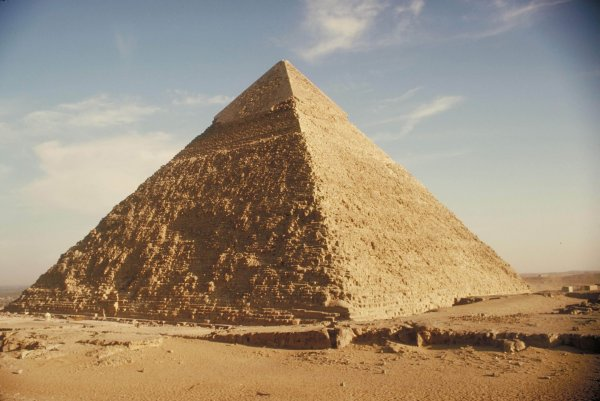
\includegraphics[width=0.65\linewidth]{GaoKao/images/2020/national_paper_1_science/q3_fig1.png}
\par}
      
        {\centering\begin{tabular*}{\linewidth}{@{}@{\extracolsep{\fill}}llll@{}}
            \(\text{A. }\dfrac{\sqrt{5}-1}{4}\)  & \(\text{B. }\dfrac{\sqrt{5}-1}{2}\)  & \(\text{C. }\dfrac{\sqrt{5}+1}{4}\)  & \(\text{D. }\dfrac{\sqrt{5}+1}{2}\)
        \end{tabular*}\par}

        \item 已知$A$为抛物线$C:y^2=2px$($p>0$)上一点，点$A$到$C$的焦点的距离为$12$，到$y$轴的距离为$9$，则$p=$(\quad)
      
        {\centering\begin{tabular*}{\linewidth}{@{}@{\extracolsep{\fill}}llll@{}}
            \(\text{A. }2\)  & \(\text{B. }3\)  & \(\text{C. }6\)  & \(\text{D. }9\)
        \end{tabular*}\par}

        \item 某校一个课外学习小组为研究某作物种子的发芽率$y$和温度$x$(单位：$^\circ$C)的关系，在$20$个不同的温度条件下进行种子发芽实验，由实验数据$(x_i,y_i)$($i=1,2,\cdots,20$)得到下面的散点图：
        {\centering
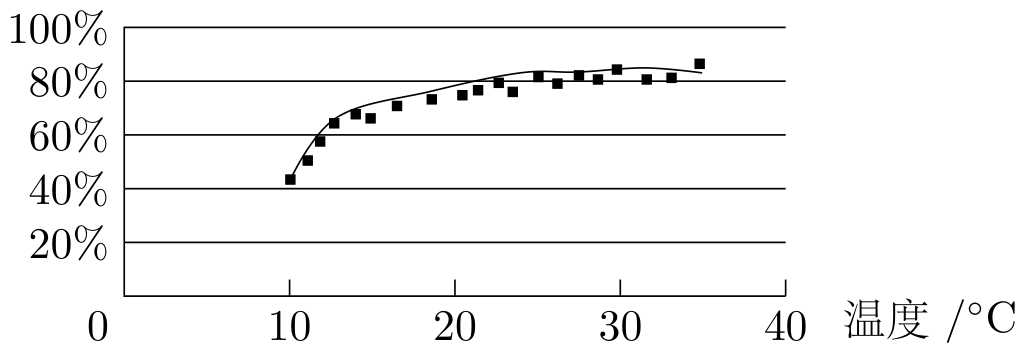
\includegraphics[width=6.1cm]{GaoKao/images/2020/national_paper_1_science/q5_fig1.png}
\par}
        由此散点图，在$10^\circ$C至$40^\circ$C之间，下面四个回归方程类型中最适宜作为发芽率$y$和温度$x$的回归方程类型的是(\quad)
      
        {\centering\begin{tabular*}{\linewidth}{@{}@{\extracolsep{\fill}}llll@{}}
            \(\text{A. }y=a+bx\)  & \(\text{B. }y=a+bx^2\)  & \(\text{C. }y=a+b\mathrm{e}^x\)  & \(\text{D. }y=a+b\ln x\)
        \end{tabular*}\par}

        \item 函数$f(x)=x^4-2x^3$的图象在点$(1,f(1))$处的切线方程为(\quad)
     
        {\centering\begin{tabular*}{\linewidth}{@{}@{\extracolsep{\fill}}llll@{}}
            \(\text{A. }y=-2x-1\)  & \(\text{B. }y=-2x+1\)  & \(\text{C. }y=2x-3\)  & \(\text{D. }y=2x+1\)
        \end{tabular*}\par}

        \item 设函数$f(x)=\cos\bigl(\omega x+\frac{\pi}{6}\bigr)$在$[-\pi,\pi]$的图象大致如下图，则$f(x)$的最小正周期为(\quad)
        {\centering
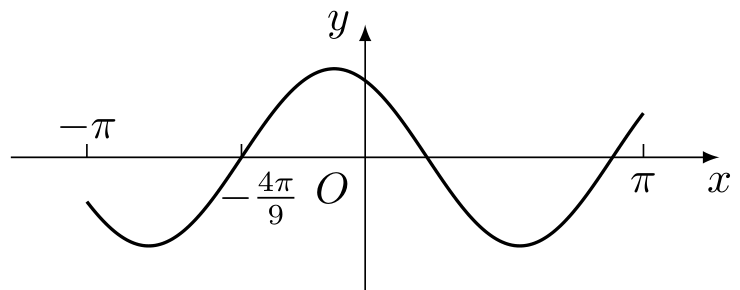
\includegraphics[width=9.0cm]{GaoKao/images/2020/national_paper_1_science/q7_fig1.png}
\par}
   
        {\centering\begin{tabular*}{\linewidth}{@{}@{\extracolsep{\fill}}llll@{}}
            \(\text{A. }\dfrac{10\pi}{9}\)  & \(\text{B. }\dfrac{7\pi}{6}\)  & \(\text{C. }\dfrac{4\pi}{3}\)  & \(\text{D. }\dfrac{3\pi}{2}\)
        \end{tabular*}\par}

        \item $\bigl(x+\dfrac{y^2}{x}\bigr)(x+y)^5$的展开式中$x^3y^3$的系数为(\quad)
    
        {\centering\begin{tabular*}{\linewidth}{@{}@{\extracolsep{\fill}}llll@{}}
            \(\text{A. }5\)  & \(\text{B. }10\)  & \(\text{C. }15\)  & \(\text{D. }20\)
        \end{tabular*}\par}

        \item 已知$\alpha\in(0,\pi)$，且$3\cos2\alpha-8\cos\alpha=5$，则$\sin\alpha=$(\quad)
       
        {\centering\begin{tabular*}{\linewidth}{@{}@{\extracolsep{\fill}}llll@{}}
            \(\text{A. }\dfrac{\sqrt{5}}{3}\)  & \(\text{B. }\dfrac{2}{3}\)  & \(\text{C. }\dfrac{1}{3}\)  & \(\text{D. }\dfrac{\sqrt{5}}{9}\)
        \end{tabular*}\par}

        \item 已知$A,B,C$为球$O$的球面上的三个点，$\odot O_1$为$\triangle ABC$的外接圆．若$\odot O_1$的面积为$4\pi$，$AB=BC=AC=OO_1$，则球$O$的表面积为(\quad)
      
        {\centering\begin{tabular*}{\linewidth}{@{}@{\extracolsep{\fill}}llll@{}}
            \(\text{A. }64\pi\)  & \(\text{B. }48\pi\)  & \(\text{C. }36\pi\)  & \(\text{D. }32\pi\)
        \end{tabular*}\par}

        \item 已知$\odot M:x^2+y^2-2x-2y-2=0$，直线$l:2x+y+2=0$，$P$为$l$上的动点，过点$P$作$\odot M$的切线$PA,PB$，切点为$A,B$，当$|PM|\cdot|AB|$最小时，直线$AB$的方程为(\quad)
      
        {\centering\begin{tabular*}{\linewidth}{@{}@{\extracolsep{\fill}}llll@{}}
            \(\text{A. }2x-y-1=0\)  & \(\text{B. }2x+y-1=0\)  & \(\text{C. }2x-y+1=0\)  & \(\text{D. }2x+y+1=0\)
        \end{tabular*}\par}

        \item 若$2^a+\log_2 a=4^b+2\log_4 b$，则(\quad)
      
        {\centering\begin{tabular*}{\linewidth}{@{}@{\extracolsep{\fill}}llll@{}}
            \(\text{A. }a>2b\)  & \(\text{B. }a<2b\)  & \(\text{C. }a>b^2\)  & \(\text{D. }a<b^2\)
        \end{tabular*}\par}
    \end{enumerate}

    \item[二、填空题]
    \begin{enumerate}[leftmargin=5pt]
        \addtocounter{enumi}{+12}
        \item 若$x,y$满足约束条件$\begin{cases}2x+y-2\leqslant 0,\\x-y-1\geqslant 0,\\y+1\geqslant 0,\end{cases}$则$z=x+7y$的最大值为\rule[-0.3ex]{3em}{0.4pt}．
        \item 设$\bm{a},\bm{b}$为单位向量，且$|\bm{a}+\bm{b}|=1$，则$|\bm{a}-\bm{b}|=\rule[-0.3ex]{3em}{0.4pt}$．
        \item 已知$F$为双曲线$C:\dfrac{x^2}{a^2}-\dfrac{y^2}{b^2}=1$($a>0,b>0$)的右焦点，$A$为$C$的右顶点，$B$为$C$上的点，且$BF$垂直于$x$轴．若$AB$的斜率为$3$，则$C$的离心率为\rule[-0.3ex]{3em}{0.4pt}．
        \item 如图，在三棱锥$P-ABC$的平面展开图中，$AC=1$，$AB=AD=\sqrt{3}$，$AB\perp AC$，$AB\perp AD$，$\angle CAE=30^\circ$，则$\cos\angle FCB=\rule[-0.3ex]{3em}{0.4pt}$．
        {\centering
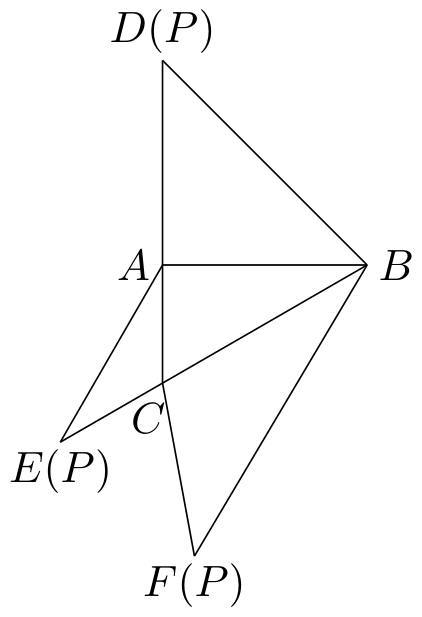
\includegraphics[width=3.6cm]{GaoKao/images/2020/national_paper_1_science/q16_fig1.png}
\par}
    \end{enumerate}

    \item[三、解答题]
    \begin{enumerate}[leftmargin=5pt]
        \addtocounter{enumi}{+16}
        \item 设$\{a_n\}$是公比不为$1$的等比数列，$a_1$为$a_2,a_3$的等差中项．
        \begin{enumerate}[label=(\arabic*)]
            \item 求$\{a_n\}$的公比；
            \item 若$a_1=1$，求数列$\{na_n\}$的前$n$项和．
        \end{enumerate}

        \item 如图，$D$为圆锥的顶点，$O$是圆锥底面的圆心，$AE$为底面直径，$AE=AD$．$\triangle ABC$是底面的内接正三角形，$P$为$DO$上一点，$PO=\dfrac{\sqrt{6}}{6}DO$．
        \begin{enumerate}[label=(\arabic*)]
            \item 证明：$PA\perp$平面$PBC$；
            \item 求二面角$B-PC-E$的余弦值．
        \end{enumerate}
        {\centering
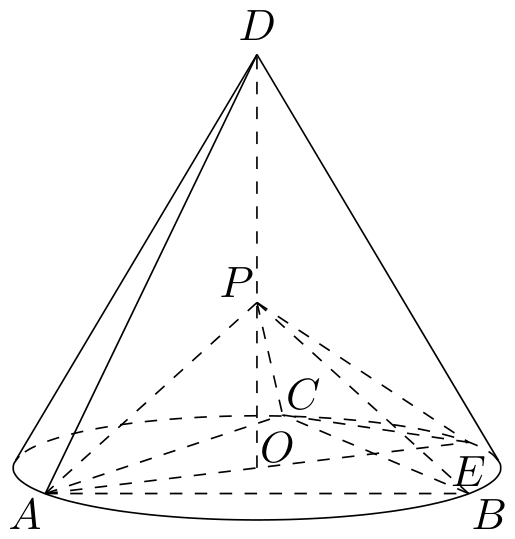
\includegraphics[width=7.3cm]{GaoKao/images/2020/national_paper_1_science/q18_fig1.png}
\par}

        \item 已知椭圆$C_1:\dfrac{x^2}{a^2}+\dfrac{y^2}{b^2}=1$($a>b>0$)的右焦点$F$与抛物线$C_2$的焦点重合，$C_1$的中心与$C_2$的顶点重合．过$F$且与$x$轴垂直的直线交$C_1$于$A,B$两点，交$C_2$于$C,D$两点，且$|CD|=\dfrac{4}{3}|AB|$．
        \begin{enumerate}[label=(\arabic*)]
            \item 求$C_1$的离心率；
            \item 设$M$是$C_1$与$C_2$的公共点，若$|MF|=5$，求$C_1$与$C_2$的标准方程．
        \end{enumerate}

        \item 如图，已知三棱柱$ABC-A_1B_1C_1$的底面是正三角形，侧面$BB_1C_1C$是矩形，$M,N$分别为$BC,B_1C_1$的中点，$P$为$AM$上一点，过$B_1C_1$和$P$的平面交$AB$于$E$，交$AC$于$F$．
        \begin{enumerate}[label=(\arabic*)]
            \item 证明：$AA_1\parallel MN$，且平面$A_1AMN\perp$平面$EB_1C_1F$；
            \item 设$O$为$\triangle A_1B_1C_1$的中心，若$AO\parallel$平面$EB_1C_1F$，且$AO=AB$，求直线$B_1E$与平面$A_1AMN$所成角的正弦值．
        \end{enumerate}
        {\centering
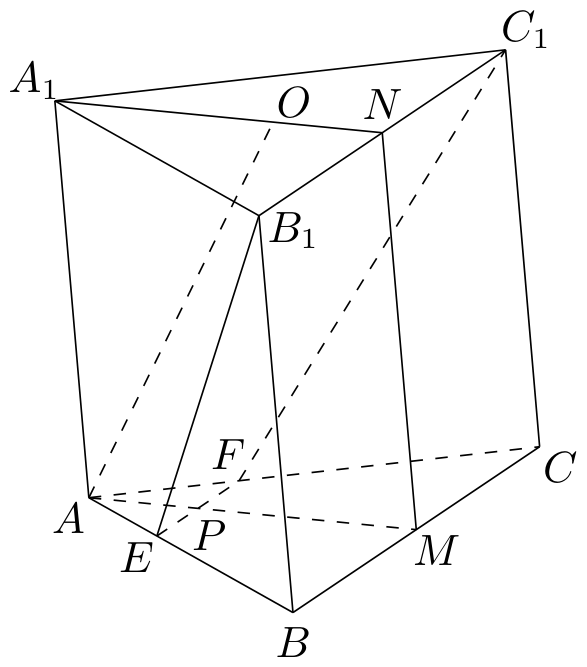
\includegraphics[width=2.0cm]{GaoKao/images/2020/national_paper_2_science/q20_fig1.png}
\par}

        \item 已知函数$f(x)=\sin^2 x\sin 2x$．
        \begin{enumerate}[label=(\arabic*)]
            \item 讨论$f(x)$在区间$(0,\pi)$的单调性；
            \item 证明：$|f(x)|\leqslant\dfrac{3\sqrt{3}}{8}$；
            \item 设$n\in\mathbb{N}^*$，证明：$\sin^2 x\sin^2 2x\sin^2 4x\cdots\sin^2 2^n x\leqslant\dfrac{3^n}{4^n}$．
        \end{enumerate}
    \end{enumerate}

    \item[四、选考题]
    \begin{enumerate}[leftmargin=5pt]
        \addtocounter{enumi}{+21}
        \item \textbf{【选修4-4：坐标系与参数方程】}已知曲线$C_1,C_2$的参数方程分别为$C_1:\begin{cases}x=4\cos^2\theta,\\y=4\sin^2\theta,\end{cases}$($\theta$为参数)，$C_2:\begin{cases}x=t+\frac{1}{t},\\y=t-\frac{1}{t},\end{cases}$($t$为参数)．
        \begin{enumerate}[label=(\arabic*)]
            \item 将$C_1,C_2$的参数方程化为普通方程；
            \item 以坐标原点为极点，$x$轴正半轴为极轴建立极坐标系．设$C_1,C_2$的交点为$P$，求圆心在极轴上，且经过极点和$P$的圆的极坐标方程．
        \end{enumerate}

        \item \textbf{【选修4-5：不等式选讲】}已知函数$f(x)=|x-a^2|+|x-2a+1|$．
        \begin{enumerate}[label=(\arabic*)]
            \item 当$a=2$时，求不等式$f(x)\geqslant 4$的解集；
            \item 若$f(x)\geqslant 4$，求$a$的取值范围．
        \end{enumerate}
    \end{enumerate}
\end{description}
\clearpage


\subsection{2020年全国I卷（文）}\label{gk:2020年全国I卷（文）}

\begin{description}
    \item[一、选择题]
    
    \begin{enumerate}[leftmargin=5pt]
        \item 已知集合$A=\{x\mid x^2-3x-4<0\}$，$B=\{-4,1,3,5\}$，则$A\cap B=$(\quad)
       
        {\centering\begin{tabular*}{\linewidth}{@{}@{\extracolsep{\fill}}llll@{}}
            \(\text{A. }\{-4,1\}\)  & \(\text{B. }\{1,5\}\)  & \(\text{C. }\{3,5\}\)  & \(\text{D. }\{1,3\}\)
        \end{tabular*}\par}

        \item 若$z=1+2\i+\i^3$，则$|z|=$(\quad)
       
        {\centering\begin{tabular*}{\linewidth}{@{}@{\extracolsep{\fill}}llll@{}}
            \(\text{A. }0\)  & \(\text{B. }1\)  & \(\text{C. }\sqrt{2}\)  & \(\text{D. }2\)
        \end{tabular*}\par}

        \item 埃及胡夫金字塔是古代世界建筑奇迹之一，它的形状可视为一个正四棱锥，以该四棱锥的高为边长的正方形面积等于该四棱锥一个侧面三角形的面积，则其侧面三角形底边上的高与底面正方形的边长的比值为(\quad)
        {\centering
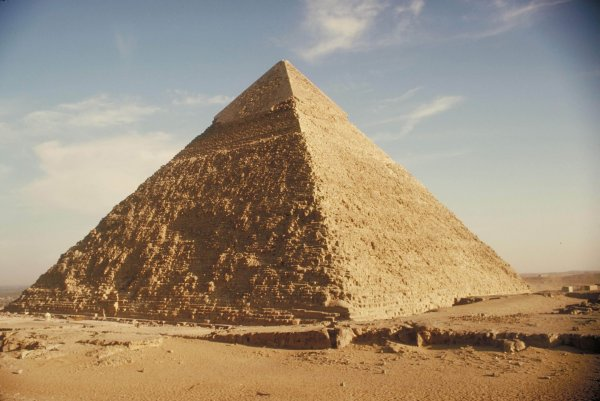
\includegraphics[width=0.65\linewidth]{GaoKao/images/2020/national_paper_1_liberal/q3_question_fig1.png}
\par}
       
        {\centering\begin{tabular*}{\linewidth}{@{}@{\extracolsep{\fill}}llll@{}}
            \(\text{A. }\dfrac{\sqrt{5}-1}{4}\)  & \(\text{B. }\dfrac{\sqrt{5}-1}{2}\)  & \(\text{C. }\dfrac{\sqrt{5}+1}{4}\)  & \(\text{D. }\dfrac{\sqrt{5}+1}{2}\)
        \end{tabular*}\par}

        \item 设$O$为正方形$ABCD$的中心，在$O,A,B,C,D$中任取$3$点，则取到的$3$点共线的概率为(\quad)
      
        {\centering\begin{tabular*}{\linewidth}{@{}@{\extracolsep{\fill}}llll@{}}
            \(\text{A. }\dfrac{1}{5}\)  & \(\text{B. }\dfrac{2}{5}\)  & \(\text{C. }\dfrac{1}{2}\)  & \(\text{D. }\dfrac{4}{5}\)
        \end{tabular*}\par}

        \item 某校一个课外学习小组为研究某作物种子的发芽率$y$和温度$x$(单位：$^\circ$C)的关系，在$20$个不同的温度条件下进行种子发芽实验，由实验数据$(x_i,y_i)$($i=1,2,\cdots,20$)得到下面的散点图：
        {\centering
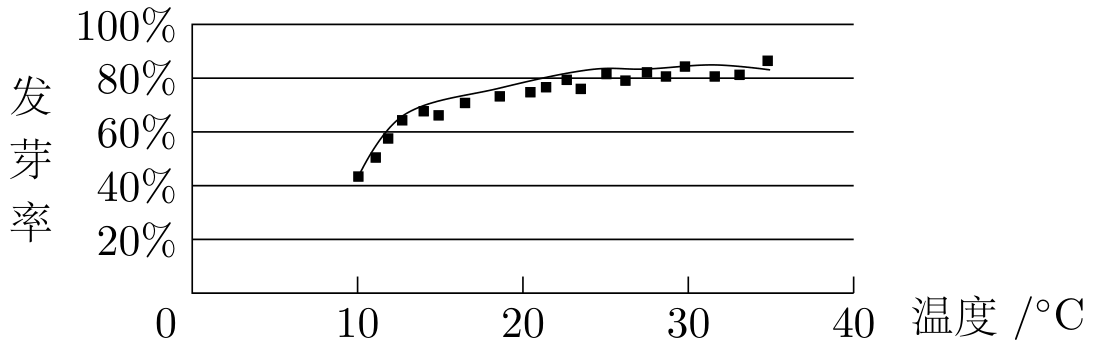
\includegraphics[width=6.5cm]{GaoKao/images/2020/national_paper_1_liberal/q5_fig1.png}
\par}
        由此散点图，在$10^\circ$C至$40^\circ$C之间，下面四个回归方程类型中最适宜作为发芽率$y$和温度$x$的回归方程类型的是(\quad)
      
        {\centering\begin{tabular*}{\linewidth}{@{}@{\extracolsep{\fill}}llll@{}}
            \(\text{A. }y=a+bx\)  & \(\text{B. }y=a+bx^2\)  & \(\text{C. }y=a+b\mathrm{e}^x\)  & \(\text{D. }y=a+b\ln x\)
        \end{tabular*}\par}

        \item 已知圆$x^2+y^2-6x=0$，过点$(1,2)$的直线被该圆所截得的弦的长度的最小值为(\quad)
      
        {\centering\begin{tabular*}{\linewidth}{@{}@{\extracolsep{\fill}}llll@{}}
            \(\text{A. }1\)  & \(\text{B. }2\)  & \(\text{C. }3\)  & \(\text{D. }4\)
        \end{tabular*}\par}

        \item 设函数$f(x)=\cos\bigl(\omega x+\frac{\pi}{6}\bigr)$在$[-\pi,\pi]$的图象大致如下图，则$f(x)$的最小正周期为(\quad)
        {\centering
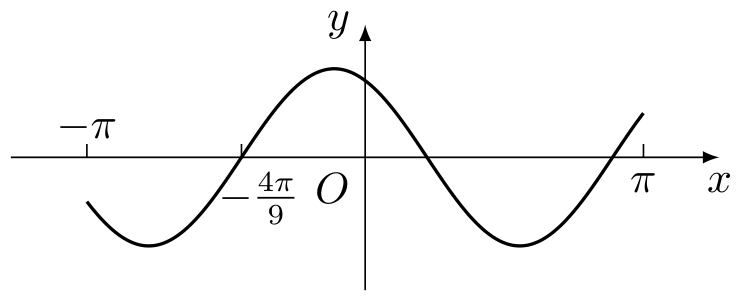
\includegraphics[width=9.0cm]{GaoKao/images/2020/national_paper_1_liberal/q7_fig1.png}
\par}
        
        {\centering\begin{tabular*}{\linewidth}{@{}@{\extracolsep{\fill}}llll@{}}
            \(\text{A. }\dfrac{10\pi}{9}\)  & \(\text{B. }\dfrac{7\pi}{6}\)  & \(\text{C. }\dfrac{4\pi}{3}\)  & \(\text{D. }\dfrac{3\pi}{2}\)
        \end{tabular*}\par}

        \item 设$a\log_3 4=2$，则$4^{-a}=$(\quad)
      
        {\centering\begin{tabular*}{\linewidth}{@{}@{\extracolsep{\fill}}llll@{}}
            \(\text{A. }\dfrac{1}{16}\)  & \(\text{B. }\dfrac{1}{9}\)  & \(\text{C. }\dfrac{1}{8}\)  & \(\text{D. }\dfrac{1}{6}\)
        \end{tabular*}\par}

        \item 执行下面的程序框图，则输出的$n=$(\quad)
        {\centering
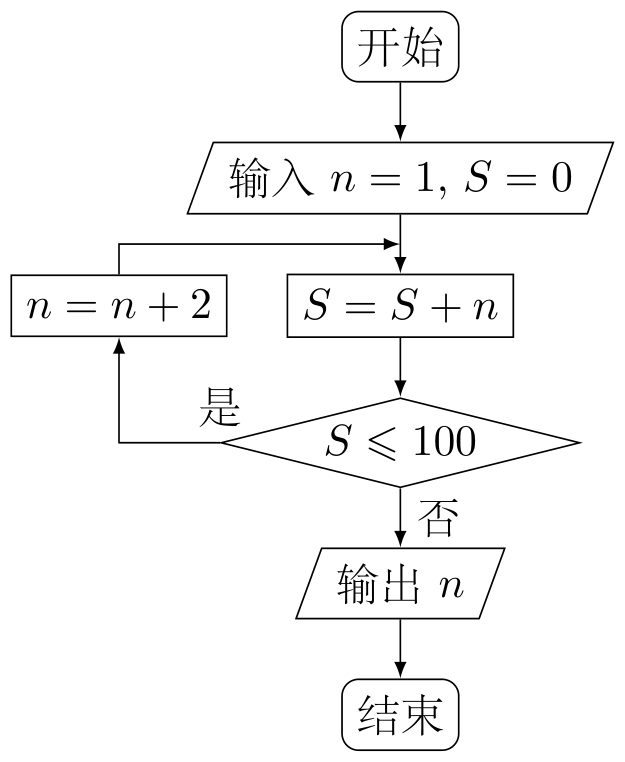
\includegraphics[width=3.4cm]{GaoKao/images/2020/national_paper_1_liberal/q9_fig1.png}
\par}
      
        {\centering\begin{tabular*}{\linewidth}{@{}@{\extracolsep{\fill}}llll@{}}
            \(\text{A. }17\)  & \(\text{B. }19\)  & \(\text{C. }21\)  & \(\text{D. }23\)
        \end{tabular*}\par}

        \item 设$\{a_n\}$是等比数列，且$a_1+a_2+a_3=1$，$a_2+a_3+a_4=2$，则$a_6+a_7+a_8=$(\quad)
      
        {\centering\begin{tabular*}{\linewidth}{@{}@{\extracolsep{\fill}}llll@{}}
            \(\text{A. }12\)  & \(\text{B. }24\)  & \(\text{C. }30\)  & \(\text{D. }32\)
        \end{tabular*}\par}

        \item 设$F_1,F_2$是双曲线$C:x^2-\dfrac{y^2}{3}=1$的两个焦点，$O$为坐标原点，点$P$在$C$上且$|OP|=2$，则$\triangle PF_1F_2$的面积为(\quad)
       
        {\centering\begin{tabular*}{\linewidth}{@{}@{\extracolsep{\fill}}llll@{}}
            \(\text{A. }\dfrac{7}{2}\)  & \(\text{B. }3\)  & \(\text{C. }\dfrac{5}{2}\)  & \(\text{D. }2\)
        \end{tabular*}\par}

        \item 已知$A,B,C$为球$O$的球面上的三个点，$\odot O_1$为$\triangle ABC$的外接圆，若$\odot O_1$的面积为$4\pi$，$AB=BC=AC=OO_1$，则球$O$的表面积为(\quad)
       
        {\centering\begin{tabular*}{\linewidth}{@{}@{\extracolsep{\fill}}llll@{}}
            \(\text{A. }64\pi\)  & \(\text{B. }48\pi\)  & \(\text{C. }36\pi\)  & \(\text{D. }32\pi\)
        \end{tabular*}\par}
    \end{enumerate}

    \item[二、填空题]
    \begin{enumerate}[leftmargin=5pt]
        \addtocounter{enumi}{+12}
        \item 若$x,y$满足约束条件$\begin{cases}2x+y-2\leqslant 0,\\x-y-1\geqslant 0,\\y+1\geqslant 0,\end{cases}$则$z=x+7y$的最大值为\rule[-0.3ex]{3em}{0.4pt}．
        \item 设向量$\bm{a}=(1,-1)$，$\bm{b}=(m+1,2m-4)$，若$\bm{a}\perp\bm{b}$，则$m=\rule[-0.3ex]{3em}{0.4pt}$．
        \item 曲线$y=\ln x+x+1$的一条切线的斜率为$2$，则该切线的方程为\rule[-0.3ex]{3em}{0.4pt}．
        \item 数列$\{a_n\}$满足$a_{n+2}+(-1)^n a_n=3n-1$，前$16$项和为$540$，则$a_1=\rule[-0.3ex]{3em}{0.4pt}$．
    \end{enumerate}

    \item[三、解答题]
    \begin{enumerate}[leftmargin=5pt]
        \addtocounter{enumi}{+16}
        \item 某厂接受了一项加工业务，加工出来的产品(单位：件)按标准分为$A,B,C,D$四个等级．加工业务约定：对于$A$级品、$B$级品、$C$级品，厂家每件分别收取加工费$90$元，$50$元，$20$元；对于$D$级品，厂家每件要赔偿原料损失费$50$元．该厂有甲、乙两个分厂可承接加工业务．甲分厂加工成本费为$25$元/件，乙分厂加工成本费为$20$元/件．厂家为决定由哪个分厂承接加工业务，在两个分厂各试加工了$100$件这种产品，并统计了这些产品的等级，整理如下：
        \begin{center}
甲分厂产品等级的频数分布表

\begin{tabular}{c|cccc}
\hline
等级 & $A$ & $B$ & $C$ & $D$ \\
\hline
频数 & 40 & 20 & 20 & 20 \\
\hline
\end{tabular}
\end{center}

\begin{center}
乙分厂产品等级的频数分布表

\begin{tabular}{c|cccc}
\hline
等级 & $A$ & $B$ & $C$ & $D$ \\
\hline
频数 & 28 & 17 & 34 & 21 \\
\hline
\end{tabular}
\end{center}
        \begin{enumerate}[label=(\arabic*)]
            \item 分别估计甲、乙两分厂加工出来的一件产品为$A$级品的概率；
            \item 分别求甲、乙两分厂加工出来的$100$件产品的平均利润，以平均利润为依据，厂家应选哪个分厂承接加工业务？
        \end{enumerate}

        \item $\triangle ABC$的内角$A,B,C$的对边分别为$a,b,c$．已知$B=150^\circ$．
        \begin{enumerate}[label=(\arabic*)]
            \item 若$a=\sqrt{3}c$，$b=2\sqrt{7}$，求$\triangle ABC$的面积；
            \item 若$\sin A+\sqrt{3}\sin C=\dfrac{\sqrt{2}}{2}$，求$C$．
        \end{enumerate}

        \item 已知椭圆$C_1:\dfrac{x^2}{a^2}+\dfrac{y^2}{b^2}=1$($a>b>0$)的右焦点$F$与抛物线$C_2$的焦点重合，$C_1$的中心与$C_2$的顶点重合．过$F$且与$x$轴垂直的直线交$C_1$于$A,B$两点，交$C_2$于$C,D$两点，且$|CD|=\dfrac{4}{3}|AB|$．
        \begin{enumerate}[label=(\arabic*)]
            \item 求$C_1$的离心率；
            \item 若$C_1$的四个顶点到$C_2$的准线距离之和为$12$，求$C_1$与$C_2$的标准方程．
        \end{enumerate}

        \item 如图，已知三棱柱$ABC-A_1B_1C_1$的底面是正三角形，侧面$BB_1C_1C$是矩形，$M,N$分别为$BC,B_1C_1$的中点，$P$为$AM$上一点，过$B_1C_1$和$P$的平面交$AB$于$E$，交$AC$于$F$．
        \begin{enumerate}[label=(\arabic*)]
            \item 证明：$AA_1\parallel MN$，且平面$A_1AMN\perp$平面$EB_1C_1F$；
            \item 设$O$为$\triangle A_1B_1C_1$的中心，若$AO=AB=6$，$AO\parallel$平面$EB_1C_1F$，且$\angle MPN=\dfrac{\pi}{3}$，求四棱锥$B-EB_1C_1F$的体积．
        \end{enumerate}
        {\centering
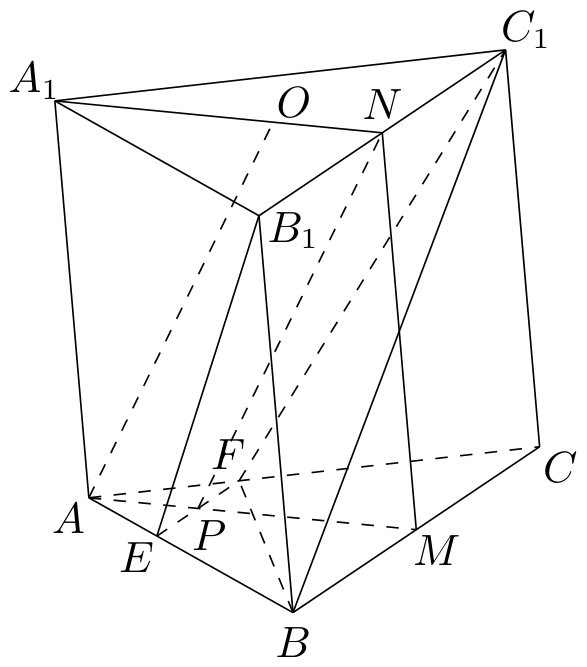
\includegraphics[width=5.6cm]{GaoKao/images/2020/national_paper_2_liberal/q20_fig1.png}
\par}

        \item 已知函数$f(x)=2\ln x+1$．
        \begin{enumerate}[label=(\arabic*)]
            \item 若$f(x)\leqslant 2x+c$，求$c$的取值范围；
            \item 设$a>0$时，讨论函数$g(x)=\dfrac{f(x)-f(a)}{x-a}$的单调性．
        \end{enumerate}
    \end{enumerate}

    \item[四、选考题]
    \begin{enumerate}[leftmargin=5pt]
        \addtocounter{enumi}{+21}
        \item \textbf{【选修4-4：坐标系与参数方程】}已知曲线$C_1,C_2$的参数方程分别为$C_1:\begin{cases}x=4\cos^2\theta,\\y=4\sin^2\theta,\end{cases}$($\theta$为参数)，$C_2:\begin{cases}x=t+\frac{1}{t},\\y=t-\frac{1}{t},\end{cases}$($t$为参数)．
        \begin{enumerate}[label=(\arabic*)]
            \item 将$C_1,C_2$的参数方程化为普通方程；
            \item 以坐标原点为极点，$x$轴正半轴为极轴建立极坐标系．设$C_1,C_2$的交点为$P$，求圆心在极轴上，且经过极点和$P$的圆的极坐标方程．
        \end{enumerate}

        \item \textbf{【选修4-5：不等式选讲】}已知函数$f(x)=|x-a^2|+|x-2a+1|$．
        \begin{enumerate}[label=(\arabic*)]
            \item 当$a=2$时，求不等式$f(x)\geqslant 4$的解集；
            \item 若$f(x)\geqslant 4$，求$a$的取值范围．
        \end{enumerate}
    \end{enumerate}
\end{description}
\clearpage


\subsection{2020年全国II卷（理）}\label{gk:2020年全国II卷（理）}

\begin{description}
    \item[一、选择题]
    \begin{enumerate}[leftmargin=5pt]
        \item 已知集合$U=\{-2,-1,0,1,2,3\}$, $A=\{-1,0,1\}$, $B=\{1,2\}$, 则$\complement_U(A\cup B)=$ (\qquad)
        
        {\centering\begin{tabular*}{\linewidth}{@{}@{\extracolsep{\fill}}llll@{}}
            \(\text{A. } \{-2,3\}\)  & \(\text{B. } \{-2,2,3\}\)  & \(\text{C. } \{-2,-1,0,3\}\)  & \(\text{D. } \{-2,-1,0,2,3\}\)
        \end{tabular*}\par}
        
        \item 若$\alpha$为第四象限角, 则 (\qquad)
        
        {\centering\begin{tabular*}{\linewidth}{@{}@{\extracolsep{\fill}}llll@{}}
            \(\text{A. } \cos 2\alpha > 0\)  & \(\text{B. } \cos 2\alpha < 0\)  & \(\text{C. } \sin 2\alpha > 0\)  & \(\text{D. } \sin 2\alpha < 0\)
        \end{tabular*}\par}
        
        \item 在新冠疫情期间, 某超市开通网上销售业务, 每天能完成$1200$份订单的配货. 由于订单量大幅增加, 导致订单积压. 为解决困难, 许多志愿者踊跃报名参加配货工作. 已知该超市某日积压$500$份订单未配货, 预计第二天的新订单超过$1600$份的概率为$0.05$. 志愿者每人每天能完成$50$份订单的配货, 为使第二天完成积压订单及当日订单的配货的概率不小于$0.95$, 则至少需要志愿者 (\qquad)
        
        {\centering\begin{tabular*}{\linewidth}{@{}@{\extracolsep{\fill}}llll@{}}
            \(\text{A. } 10\text{名}\)  & \(\text{B. } 18\text{名}\)  & \(\text{C. } 24\text{名}\)  & \(\text{D. } 32\text{名}\)
        \end{tabular*}\par}
        
        \item 北京天坛的圜丘坛为古代祭天的场所, 分上、中、下三层, 上层中心有一块圆形石板(称为天心石), 环绕天心石砌$9$块扇面形石板构成第一环, 向外每环依次增加$9$块, 下一层的第一环比上一层的最后一环多$9$块, 向外每环依次也增加$9$块. 已知每层环数相同, 且下层比中层多$729$块, 则三层共有扇面形石板(不含天心石) (\qquad)
        
        {\centering\begin{tabular*}{\linewidth}{@{}@{\extracolsep{\fill}}llll@{}}
            \(\text{A. } 3699\text{块}\)  & \(\text{B. } 3474\text{块}\)  & \(\text{C. } 3402\text{块}\)  & \(\text{D. } 3339\text{块}\)
        \end{tabular*}\par}
        
        \item 若过点$(2,1)$的圆与两坐标轴都相切, 则圆心到直线$2x-y-3=0$的距离为 (\qquad)
        
        {\centering\begin{tabular*}{\linewidth}{@{}@{\extracolsep{\fill}}llll@{}}
            \(\text{A. } \dfrac{\sqrt{5}}{5}\)  & \(\text{B. } \dfrac{2\sqrt{5}}{5}\)  & \(\text{C. } \dfrac{3\sqrt{5}}{5}\)  & \(\text{D. } \dfrac{4\sqrt{5}}{5}\)
        \end{tabular*}\par}
        
        \item 数列$\{a_n\}$中, $a_1=2$, $a_{m+n}=a_m a_n$. 若$a_{k+1}+a_{k+2}+\cdots+a_{k+10}=2^{15}-2^{5}$, 则$k=$ (\qquad)
        
        {\centering\begin{tabular*}{\linewidth}{@{}@{\extracolsep{\fill}}llll@{}}
            \(\text{A. } 2\)  & \(\text{B. } 3\)  & \(\text{C. } 4\)  & \(\text{D. } 5\)
        \end{tabular*}\par}
        
        \item 如图是一个多面体的三视图, 这个多面体某条棱的一个端点在正视图中对应的点为$M$, 在俯视图中对应的点为$N$, 则该端点在侧视图中对应的点为 (\qquad)
        
        {\centering
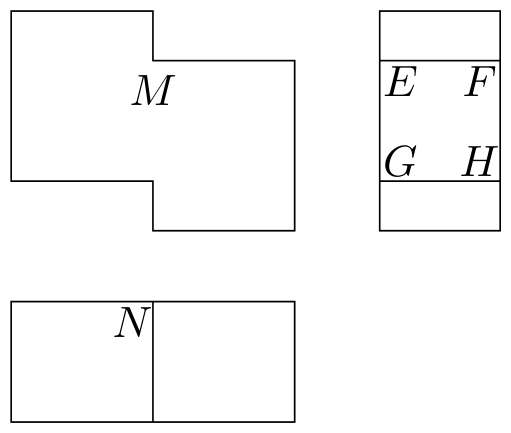
\includegraphics[width=6.2cm]{GaoKao/images/2020/national_paper_2_science/q7_fig1.png}
\par}
        
        {\centering\begin{tabular*}{\linewidth}{@{}@{\extracolsep{\fill}}llll@{}}
            \(\text{A. } E\)  & \(\text{B. } F\)  & \(\text{C. } G\)  & \(\text{D. } H\)
        \end{tabular*}\par}
        
        \item 设$O$为坐标原点, 直线$x=a$与双曲线$C:\dfrac{x^{2}}{a^{2}}-\dfrac{y^{2}}{b^{2}}=1$ $(a>0,b>0)$的两条渐近线分别交于$D,E$两点. 若$\triangle ODE$的面积为$8$, 则$C$的焦距的最小值为 (\qquad)
        
        {\centering\begin{tabular*}{\linewidth}{@{}@{\extracolsep{\fill}}llll@{}}
            \(\text{A. } 4\)  & \(\text{B. } 8\)  & \(\text{C. } 16\)  & \(\text{D. } 32\)
        \end{tabular*}\par}
        
        \item 设函数$f(x)=\ln|2x+1|-\ln|2x-1|$, 则$f(x)$ (\qquad)
        
        {\centering\begin{tabular*}{\linewidth}{@{}@{\extracolsep{\fill}}llll@{}}
            \(\text{A. } \text{是偶函数, 且在}\bigl(\frac{1}{2},+\infty\bigr)\text{单调递增}\)  & \(\text{B. } \text{是奇函数, 且在}\bigl(-\frac{1}{2},\frac{1}{2}\bigr)\text{单调递减}\)  \\
            \(\text{C. } \text{是偶函数, 且在}\bigl(-\infty,-\frac{1}{2}\bigr)\text{单调递增}\)  & \(\text{D. } \text{是奇函数, 且在}\bigl(-\infty,-\frac{1}{2}\bigr)\text{单调递减}\)
        \end{tabular*}\par}
        
        \item 已知$\triangle ABC$是面积为$\dfrac{9\sqrt{3}}{4}$的等边三角形, 且其顶点都在球$O$的球面上. 若球$O$的表面积为$16\pi$, 则$O$到平面$ABC$的距离为 (\qquad)
        
        {\centering\begin{tabular*}{\linewidth}{@{}@{\extracolsep{\fill}}llll@{}}
            \(\text{A. } \sqrt{3}\)  & \(\text{B. } \dfrac{3}{2}\)  & \(\text{C. } 1\)  & \(\text{D. } \dfrac{\sqrt{3}}{2}\)
        \end{tabular*}\par}
        
        \item 若$2^{x}-2^{y}<3^{-x}-3^{-y}$, 则 (\qquad)
        
        {\centering\begin{tabular*}{\linewidth}{@{}@{\extracolsep{\fill}}llll@{}}
            \(\text{A. } \ln(y-x+1)>0\)  & \(\text{B. } \ln(y-x+1)<0\)  & \(\text{C. } \ln|x-y|>0\)  & \(\text{D. } \ln|x-y|<0\)
        \end{tabular*}\par}
        
        \item $0$--$1$周期序列在通信技术中有着重要应用. 若序列$a_1a_2\cdots a_n\cdots$满足$a_i\in\{0,1\}$ $(i=1,2,\cdots)$, 且存在正整数$m$, 使得$a_{i+m}=a_i$ $(i=1,2,\cdots)$成立, 则称其为$0$--$1$周期序列, 并称满足$a_{i+m}=a_i$ $(i=1,2,\cdots)$的最小正整数$m$为这个序列的周期. 对于周期为$m$的$0$--$1$序列$a_1a_2\cdots a_n\cdots$, $C(k)=\dfrac{1}{m}\displaystyle\sum_{i=1}^{m}a_i a_{i+k}$ $(k=1,2,\cdots,m-1)$是描述其性质的重要指标. 下列周期为$5$的$0$--$1$序列中, 满足$C(k)\leqslant\dfrac{1}{5}$ $(k=1,2,3,4)$的序列是 (\qquad)
        
        {\centering\begin{tabular*}{\linewidth}{@{}@{\extracolsep{\fill}}llll@{}}
            \(\text{A. } 11010\cdots\)  & \(\text{B. } 11011\cdots\)  & \(\text{C. } 10001\cdots\)  & \(\text{D. } 11001\cdots\)
        \end{tabular*}\par}
        
    \end{enumerate}
    
    \item[二、填空题]
    \begin{enumerate}[leftmargin=5pt]
      \addtocounter{enumi}{+12}
        \item 已知单位向量$\bm{a},\bm{b}$的夹角为$45^{\circ}$, $k\bm{a}-\bm{b}$与$\bm{a}$垂直, 则$k=$ \rule[-0.3ex]{3em}{0.4pt}.
        \item $4$名同学到$3$个小区参加垃圾分类宣传活动, 每名同学只去$1$个小区, 每个小区至少安排$1$名同学, 则不同的安排方法共有 \rule[-0.3ex]{3em}{0.4pt} 种.
        \item 设复数$z_1,z_2$满足$|z_1|=|z_2|=2$, $z_1+z_2=\sqrt{3}+\i$, 则$|z_1-z_2|=$ \rule[-0.3ex]{3em}{0.4pt}.
        \item 设有下列四个命题:\\
        $p_1$: 两两相交且不过同一点的三条直线必在同一平面内;\\
        $p_2$: 过空间中任意三点有且仅有一个平面;\\
        $p_3$: 若空间两条直线不相交, 则这两条直线平行;\\
        $p_4$: 若直线$l\subset$平面$\alpha$, 直线$m\perp$平面$\alpha$, 则$m\perp l$.\\
        则下述命题中所有真命题的序号是 \rule[-0.3ex]{3em}{0.4pt}.\\
        \ding{172} $p_1\land p_4$; \quad \ding{173} $\neg p_1\land p_2$; \quad \ding{174} $p_2\lor\neg p_3$; \quad \ding{175} $\neg p_3\lor\neg p_4$.
    \end{enumerate}
    
    \item[三、解答题]
    \begin{enumerate}[leftmargin=5pt]
      \addtocounter{enumi}{+16}
        \item $\triangle ABC$中, $\sin^{2}A-\sin^{2}B-\sin^{2}C=\sin B\sin C$.
        \begin{enumerate}[label=(\arabic*)]
            \item 求$A$;
            \item 若$BC=3$, 求$\triangle ABC$周长的最大值.
        \end{enumerate}

        \item 某沙漠地区经过治理, 生态系统得到很大改善, 野生动物数量有所增加. 为调查该地区某种野生动物的数量, 将其分成面积相近的$200$个地块, 从这些地块中用简单随机抽样的方法抽取$20$个作为样区, 调查得到样本数据$(x_i,y_i)$ $(i=1,2,\cdots,20)$, 其中$x_i$和$y_i$分别表示第$i$个样区的植物覆盖面积(单位: 公顷)和这种野生动物的数量, 并计算得$\displaystyle\sum_{i=1}^{20}x_i=60$, $\displaystyle\sum_{i=1}^{20}y_i=1200$, $\displaystyle\sum_{i=1}^{20}(x_i-\bar{x})^{2}=80$, $\displaystyle\sum_{i=1}^{20}(y_i-\bar{y})^{2}=9000$, $\displaystyle\sum_{i=1}^{20}(x_i-\bar{x})(y_i-\bar{y})=800$.
        \begin{enumerate}[label=(\arabic*)]
            \item 求该地区这种野生动物数量的估计值(这种野生动物数量的估计值等于样区这种野生动物数量的平均数乘以地块数);
            \item 求样本$(x_i,y_i)$ $(i=1,2,\cdots,20)$的相关系数(精确到$0.01$);
            \item 根据现有统计资料, 各地块间植物覆盖面积差异很大. 为提高样本的代表性以获得该地区这种野生动物数量更准确的估计, 请给出一种你认为更合理的抽样方法, 并说明理由.
        \end{enumerate}
        
        附: 相关系数$r=\dfrac{\displaystyle\sum_{i=1}^{n}(x_i-\bar{x})(y_i-\bar{y})}{\sqrt{\displaystyle\sum_{i=1}^{n}(x_i-\bar{x})^{2}\displaystyle\sum_{i=1}^{n}(y_i-\bar{y})^{2}}}$, $\sqrt{2}\approx 1.414$.
        
        \item 已知椭圆$C_1:\dfrac{x^{2}}{a^{2}}+\dfrac{y^{2}}{b^{2}}=1$ $(a>b>0)$的右焦点$F$与抛物线$C_2$的焦点重合, $C_1$的中心与$C_2$的顶点重合. 过$F$且与$x$轴垂直的直线交$C_1$于$A,B$两点, 交$C_2$于$C,D$两点, 且$|CD|=\dfrac{4}{3}|AB|$.
        \begin{enumerate}[label=(\arabic*)]
            \item 求$C_1$的离心率;
            \item 设$M$是$C_1$与$C_2$的公共点, 若$|MF|=5$, 求$C_1$与$C_2$的标准方程.
        \end{enumerate}
        
        \item 如图, 已知三棱柱$ABC-A_1B_1C_1$的底面是正三角形, 侧面$BB_1C_1C$是矩形, $M,N$分别为$BC,B_1C_1$的中点, $P$为$AM$上一点. 过$B_1C_1$和$P$的平面交$AB$于$E$, 交$AC$于$F$.
        
        {\centering
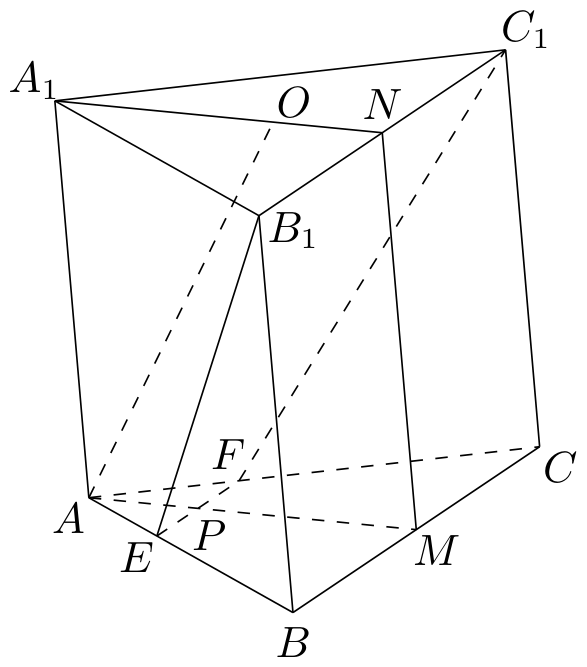
\includegraphics[width=2.0cm]{GaoKao/images/2020/national_paper_2_science/q20_fig1.png}
\par}
        
        \begin{enumerate}[label=(\arabic*)]
            \item 证明: $AA_1\parallel MN$, 且平面$A_1AMN\perp$平面$EB_1C_1F$;
            \item 设$O$为$\triangle A_1B_1C_1$的中心, 若$AO\parallel$平面$EB_1C_1F$, 且$AO=AB$, 求直线$B_1E$与平面$A_1AMN$所成角的正弦值.
        \end{enumerate}
        
        \item 已知函数$f(x)=\sin^{2}x\sin 2x$.
        \begin{enumerate}[label=(\arabic*)]
            \item 讨论$f(x)$在区间$(0,\pi)$的单调性;
            \item 证明: $|f(x)|\leqslant\dfrac{3\sqrt{3}}{8}$;
            \item 设$n\in\mathbb{N}^{*}$, 证明: $\sin^{2}x\sin^{2}2x\sin^{2}4x\cdots\sin^{2}2^{n}x\leqslant\dfrac{3^{n}}{4^{n}}$.
        \end{enumerate}
        
        \item 已知曲线$C_1,C_2$的参数方程分别为$C_1:\begin{cases}x=4\cos^{2}\theta,\\y=4\sin^{2}\theta;\end{cases}$ ($\theta$为参数), $C_2:\begin{cases}x=t+\dfrac{1}{t},\\[6pt]y=t-\dfrac{1}{t};\end{cases}$ ($t$为参数).
        \begin{enumerate}[label=(\arabic*)]
            \item 将$C_1,C_2$的参数方程化为普通方程;
            \item 以坐标原点为极点, $x$轴正半轴为极轴建立极坐标系. 设$C_1,C_2$的交点为$P$, 求圆心在极轴上, 且经过极点和$P$的圆的极坐标方程.
        \end{enumerate}
        
        \item 已知函数$f(x)=|x-a^{2}|+|x-2a+1|$.
        \begin{enumerate}[label=(\arabic*)]
            \item 当$a=2$时, 求不等式$f(x)\geqslant 4$的解集;
            \item 若$f(x)\geqslant 4$, 求$a$的取值范围.
        \end{enumerate}
        
    \end{enumerate}
\end{description}
\clearpage


\subsection{2020年全国II卷（文）}\label{gk:2020年全国II卷（文）}

\begin{description}
    \item[一、选择题]
    \begin{enumerate}[leftmargin=5pt]
        \item 已知集合$A=\{x\mid|x|<3,\;x\in\mathbb{Z}\}$, $B=\{x\mid|x|>1,\;x\in\mathbb{Z}\}$, 则$A\cap B=$ (\qquad)
        
        {\centering\begin{tabular*}{\linewidth}{@{}@{\extracolsep{\fill}}llll@{}}
            \(\text{A. } \varnothing\)  & \(\text{B. } \{-3,-2,2,3\}\)  & \(\text{C. } \{-2,0,2\}\)  & \(\text{D. } \{-2,2\}\)
        \end{tabular*}\par}
        
        \item $(1-\i)^{4}=$ (\qquad)
        
        {\centering\begin{tabular*}{\linewidth}{@{}@{\extracolsep{\fill}}llll@{}}
            \(\text{A. } -4\)  & \(\text{B. } 4\)  & \(\text{C. } -4\i\)  & \(\text{D. } 4\i\)
        \end{tabular*}\par}
        
        \item 如图, 将钢琴上的$12$个键依次记为$a_1,a_2,\cdots,a_{12}$. 设$1\leqslant i<j<k\leqslant 12$. 若$k-j=3$且$j-i=4$, 则称$a_i,a_j,a_k$为原位大三和弦; 若$k-j=4$且$j-i=3$, 则称$a_i,a_j,a_k$为原位小三和弦. 用这$12$个键可以构成的原位大三和弦与原位小三和弦的个数之和为 (\qquad)
        
        {\centering
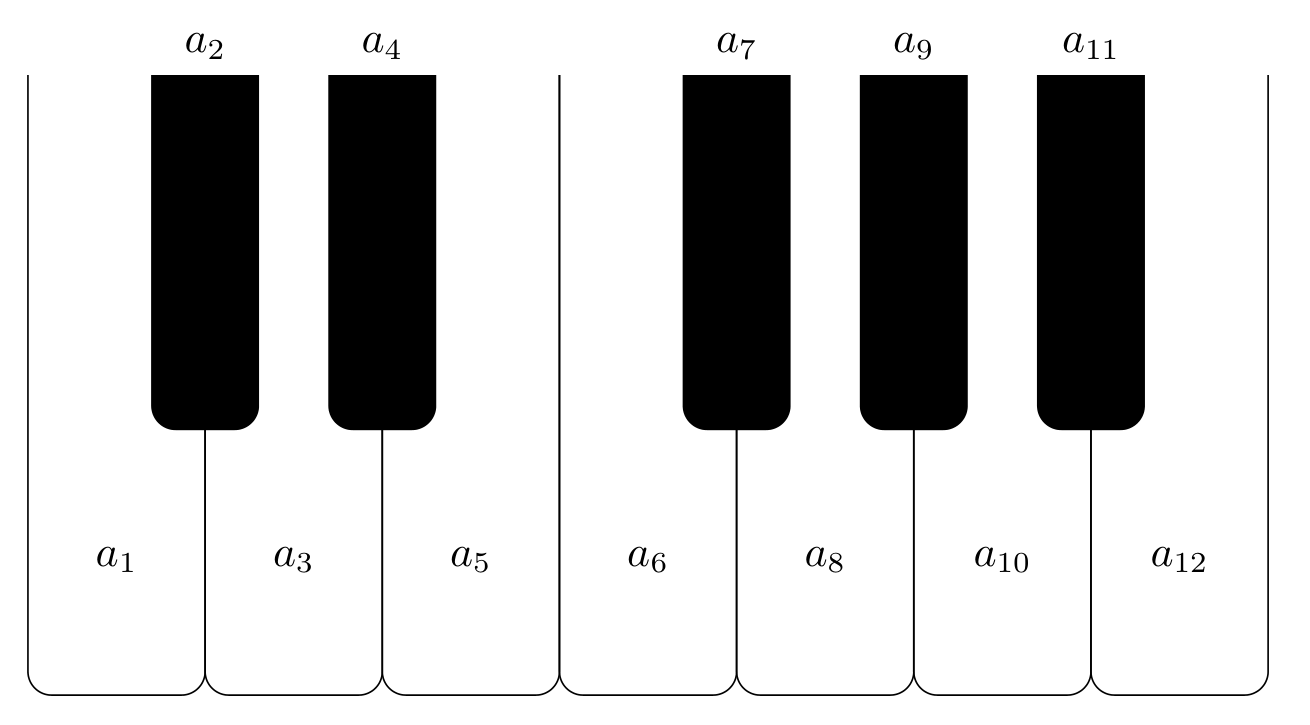
\includegraphics[width=14.0cm]{GaoKao/images/2020/national_paper_2_liberal/q3_fig1.png}
\par}
        
        {\centering\begin{tabular*}{\linewidth}{@{}@{\extracolsep{\fill}}llll@{}}
            \(\text{A. } 5\)  & \(\text{B. } 8\)  & \(\text{C. } 10\)  & \(\text{D. } 15\)
        \end{tabular*}\par}
        
        \item 在新冠疫情期间, 某超市开通网上销售业务, 每天能完成$1200$份订单的配货. 由于订单量大幅增加, 导致订单积压. 为解决困难, 许多志愿者踊跃报名参加配货工作. 已知该超市某日积压$500$份订单未配货, 预计第二天的新订单超过$1600$份的概率为$0.05$, 志愿者每人每天能完成$50$份订单的配货, 为使第二天完成积压订单及当日订单的配货的概率不小于$0.95$, 则至少需要志愿者 (\qquad)
        
        {\centering\begin{tabular*}{\linewidth}{@{}@{\extracolsep{\fill}}llll@{}}
            \(\text{A. } 10\text{名}\)  & \(\text{B. } 18\text{名}\)  & \(\text{C. } 24\text{名}\)  & \(\text{D. } 32\text{名}\)
        \end{tabular*}\par}
        
        \item 已知单位向量$\bm{a},\bm{b}$的夹角为$60^{\circ}$, 则在下列向量中, 与$\bm{b}$垂直的是 (\qquad)
        
        {\centering\begin{tabular*}{\linewidth}{@{}@{\extracolsep{\fill}}llll@{}}
            \(\text{A. } \bm{a}+2\bm{b}\)  & \(\text{B. } 2\bm{a}+\bm{b}\)  & \(\text{C. } \bm{a}-2\bm{b}\)  & \(\text{D. } 2\bm{a}-\bm{b}\)
        \end{tabular*}\par}
        
        \item 设$S_n$为等比数列$\{a_n\}$的前$n$项和. 若$a_5-a_3=12$, $a_6-a_4=24$, 则$\dfrac{S_n}{a_n}=$ (\qquad)
        
        {\centering\begin{tabular*}{\linewidth}{@{}@{\extracolsep{\fill}}llll@{}}
            \(\text{A. } 2^{n}-1\)  & \(\text{B. } 2-2^{1-n}\)  & \(\text{C. } 2-2^{n-1}\)  & \(\text{D. } 2^{1-n}-1\)
        \end{tabular*}\par}
        
        \item 执行下面的程序框图, 若输入的$k=0$, $a=0$, 则输出的$k$为 (\qquad)
        
        {\centering
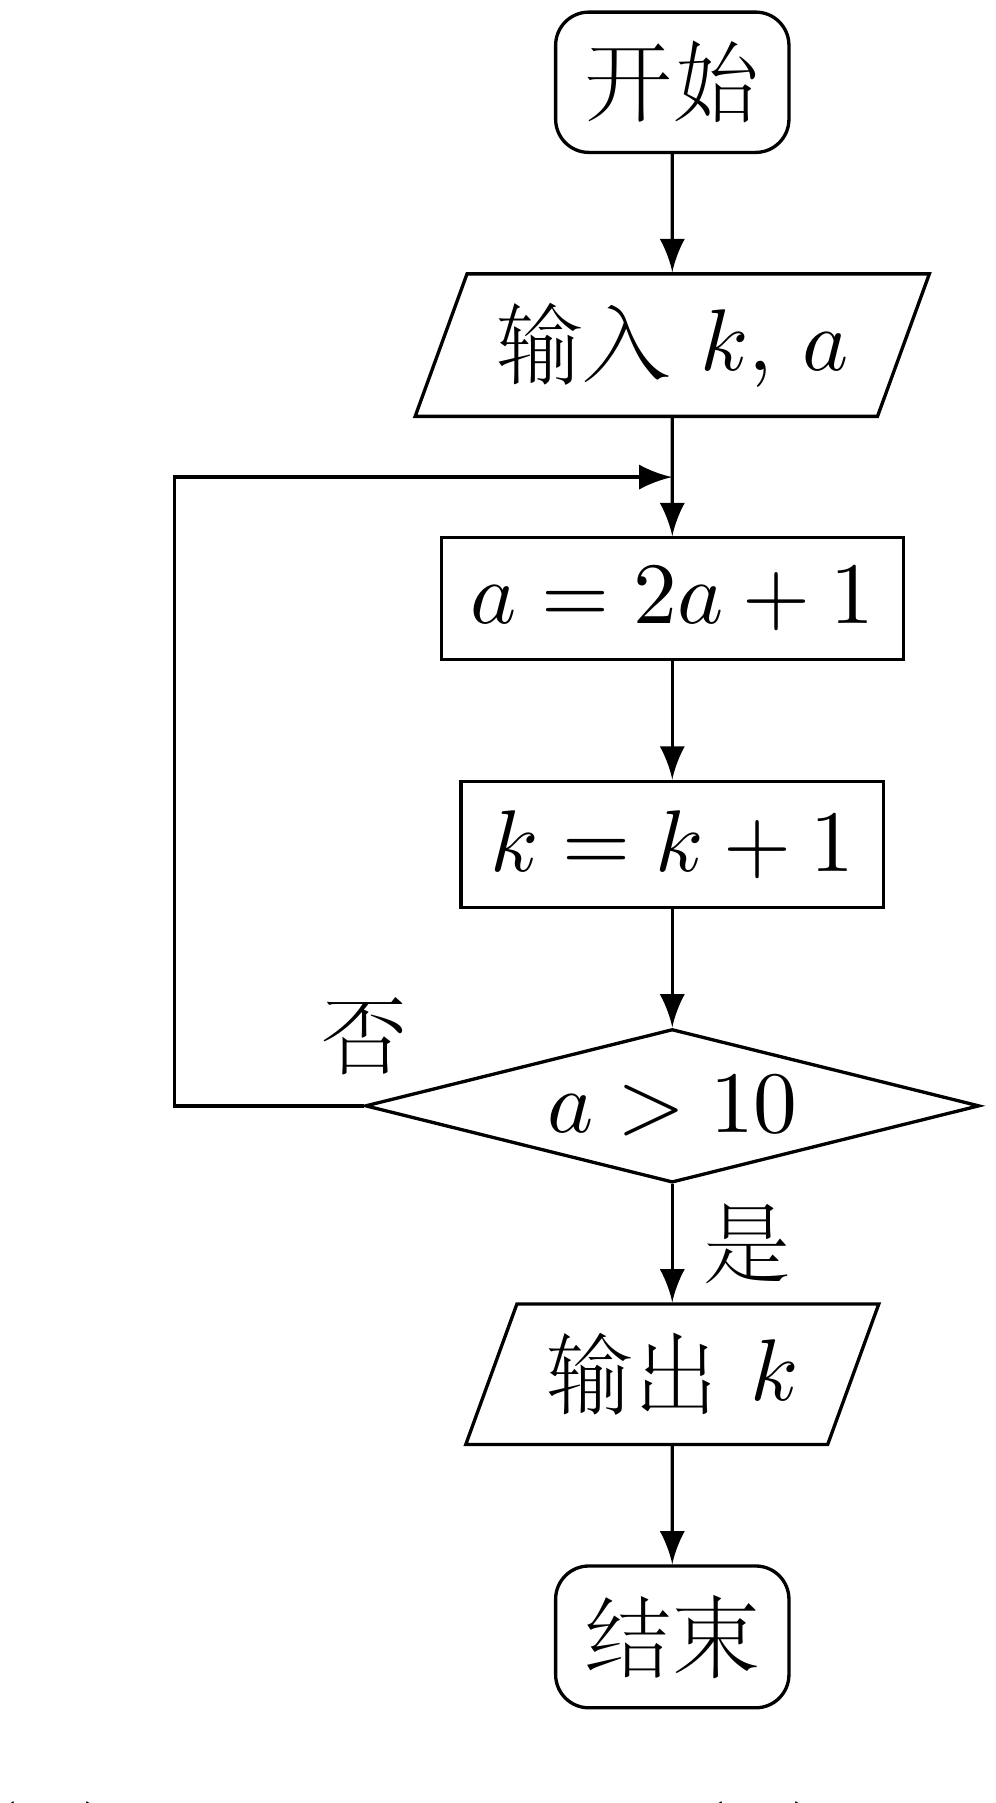
\includegraphics[width=2.9cm]{GaoKao/images/2020/national_paper_2_liberal/q7_fig1.png}
\par}
        
        {\centering\begin{tabular*}{\linewidth}{@{}@{\extracolsep{\fill}}llll@{}}
            \(\text{A. } 2\)  & \(\text{B. } 3\)  & \(\text{C. } 4\)  & \(\text{D. } 5\)
        \end{tabular*}\par}
        
        \item 若过点$(2,1)$的圆与两坐标轴都相切, 则圆心到直线$2x-y-3=0$的距离为 (\qquad)
        
        {\centering\begin{tabular*}{\linewidth}{@{}@{\extracolsep{\fill}}llll@{}}
            \(\text{A. } \dfrac{\sqrt{5}}{5}\)  & \(\text{B. } \dfrac{2\sqrt{5}}{5}\)  & \(\text{C. } \dfrac{3\sqrt{5}}{5}\)  & \(\text{D. } \dfrac{4\sqrt{5}}{5}\)
        \end{tabular*}\par}
        
        \item 设$O$为坐标原点, 直线$x=a$与双曲线$C:\dfrac{x^{2}}{a^{2}}-\dfrac{y^{2}}{b^{2}}=1$ $(a>0,b>0)$的两条渐近线分别交于$D,E$两点. 若$\triangle ODE$的面积为$8$, 则$C$的焦距的最小值为 (\qquad)
        
        {\centering\begin{tabular*}{\linewidth}{@{}@{\extracolsep{\fill}}llll@{}}
            \(\text{A. } 4\)  & \(\text{B. } 8\)  & \(\text{C. } 16\)  & \(\text{D. } 32\)
        \end{tabular*}\par}
        
        \item 设函数$f(x)=x^{3}-\dfrac{1}{x^{3}}$, 则$f(x)$ (\qquad)
        
        {\centering\begin{tabular*}{\linewidth}{@{}@{\extracolsep{\fill}}llll@{}}
            \(\text{A. } \text{是奇函数, 且在}(0,+\infty)\text{单调递增}\)  & \(\text{B. } \text{是奇函数, 且在}(0,+\infty)\text{单调递减}\)  \\
            \(\text{C. } \text{是偶函数, 且在}(0,+\infty)\text{单调递增}\)  & \(\text{D. } \text{是偶函数, 且在}(0,+\infty)\text{单调递减}\)
        \end{tabular*}\par}
        
        \item 已知$\triangle ABC$是面积为$\dfrac{9\sqrt{3}}{4}$的等边三角形, 且其顶点都在球$O$的球面上. 若球$O$的表面积为$16\pi$, 则$O$到平面$ABC$的距离为 (\qquad)
        
        {\centering\begin{tabular*}{\linewidth}{@{}@{\extracolsep{\fill}}llll@{}}
            \(\text{A. } \sqrt{3}\)  & \(\text{B. } \dfrac{3}{2}\)  & \(\text{C. } 1\)  & \(\text{D. } \dfrac{\sqrt{3}}{2}\)
        \end{tabular*}\par}
        
        \item 若$2^{x}-2^{y}<3^{-x}-3^{-y}$, 则 (\qquad)
        
        {\centering\begin{tabular*}{\linewidth}{@{}@{\extracolsep{\fill}}llll@{}}
            \(\text{A. } \ln(y-x+1)>0\)  & \(\text{B. } \ln(y-x+1)<0\)  & \(\text{C. } \ln|x-y|>0\)  & \(\text{D. } \ln|x-y|<0\)
        \end{tabular*}\par}
        
    \end{enumerate}
    
    \item[二、填空题]
    \begin{enumerate}[leftmargin=5pt]
      \addtocounter{enumi}{+12}
        \item 若$\sin x=-\dfrac{2}{3}$, 则$\cos 2x=$ \rule[-0.3ex]{3em}{0.4pt}.
        \item 设$S_n$为等差数列$\{a_n\}$的前$n$项和. 若$a_1=-2$, $a_2+a_6=2$, 则$S_{10}=$ \rule[-0.3ex]{3em}{0.4pt}.
        \item 若$x,y$满足约束条件$\begin{cases}x+y\geqslant -1,\\x-y\geqslant -1,\\2x-y\leqslant 1,\end{cases}$ 则$z=x+2y$的最大值是 \rule[-0.3ex]{3em}{0.4pt}.
        \item 设有下列四个命题:\\
        $p_1$: 两两相交且不过同一点的三条直线必在同一平面内;\\
        $p_2$: 过空间中任意三点有且仅有一个平面;\\
        $p_3$: 若空间两条直线不相交, 则这两条直线平行;\\
        $p_4$: 若直线$l\subset$平面$\alpha$, 直线$m\perp$平面$\alpha$, 则$m\perp l$.\\
        则下述命题中所有真命题的序号是 \rule[-0.3ex]{3em}{0.4pt}.\\
        \ding{172} $p_1\land p_4$; \quad \ding{173} $\neg p_1\land p_2$; \quad \ding{174} $p_2\lor\neg p_3$; \quad \ding{175} $\neg p_3\lor\neg p_4$.
    \end{enumerate}
    
    \item[三、解答题]
    \begin{enumerate}[leftmargin=5pt]
      \addtocounter{enumi}{+16}
        \item $\triangle ABC$的内角$A,B,C$的对边分别为$a,b,c$, 已知$\cos^{2}\bigl(\dfrac{\pi}{2}+A\bigr)+\cos A=\dfrac{5}{4}$.
        \begin{enumerate}[label=(\arabic*)]
            \item 求$A$;
            \item 若$b-c=\dfrac{\sqrt{3}}{3}a$, 证明: $\triangle ABC$是直角三角形.
        \end{enumerate}

        \item 某沙漠地区经过治理, 生态系统得到很大改善, 野生动物数量有所增加. 为调查该地区某种野生动物的数量, 将其分成面积相近的$200$个地块, 从这些地块中用简单随机抽样的方法抽取$20$个作为样区, 调查得到样本数据$(x_i,y_i)$ $(i=1,2,\cdots,20)$, 其中$x_i$和$y_i$分别表示第$i$个样区的植物覆盖面积(单位: 公顷)和这种野生动物的数量, 并计算得$\displaystyle\sum_{i=1}^{20}x_i=60$, $\displaystyle\sum_{i=1}^{20}y_i=1200$, $\displaystyle\sum_{i=1}^{20}(x_i-\bar{x})^{2}=80$, $\displaystyle\sum_{i=1}^{20}(y_i-\bar{y})^{2}=9000$, $\displaystyle\sum_{i=1}^{20}(x_i-\bar{x})(y_i-\bar{y})=800$.
        \begin{enumerate}[label=(\arabic*)]
            \item 求该地区这种野生动物数量的估计值(这种野生动物数量的估计值等于样区这种野生动物数量的平均数乘以地块数);
            \item 求样本$(x_i,y_i)$ $(i=1,2,\cdots,20)$的相关系数(精确到$0.01$);
            \item 根据现有统计资料, 各地块间植物覆盖面积差异很大. 为提高样本的代表性以获得该地区这种野生动物数量更准确的估计, 请给出一种你认为更合理的抽样方法, 并说明理由.
        \end{enumerate}
        
        附: 相关系数$r=\dfrac{\displaystyle\sum_{i=1}^{n}(x_i-\bar{x})(y_i-\bar{y})}{\sqrt{\displaystyle\sum_{i=1}^{n}(x_i-\bar{x})^{2}\displaystyle\sum_{i=1}^{n}(y_i-\bar{y})^{2}}}$, $\sqrt{2}\approx 1.414$.
        
        \item 已知椭圆$C_1:\dfrac{x^{2}}{a^{2}}+\dfrac{y^{2}}{b^{2}}=1$ $(a>b>0)$的右焦点$F$与抛物线$C_2$的焦点重合, $C_1$的中心与$C_2$的顶点重合. 过$F$且与$x$轴垂直的直线交$C_1$于$A,B$两点, 交$C_2$于$C,D$两点, 且$|CD|=\dfrac{4}{3}|AB|$.
        \begin{enumerate}[label=(\arabic*)]
            \item 求$C_1$的离心率;
            \item 若$C_1$的四个顶点到$C_2$的准线距离之和为$12$, 求$C_1$与$C_2$的标准方程.
        \end{enumerate}
        
        \item 如图, 已知三棱柱$ABC-A_1B_1C_1$的底面是正三角形, 侧面$BB_1C_1C$是矩形, $M,N$分别为$BC,B_1C_1$的中点, $P$为$AM$上一点. 过$B_1C_1$和$P$的平面交$AB$于$E$, 交$AC$于$F$.
        
        {\centering
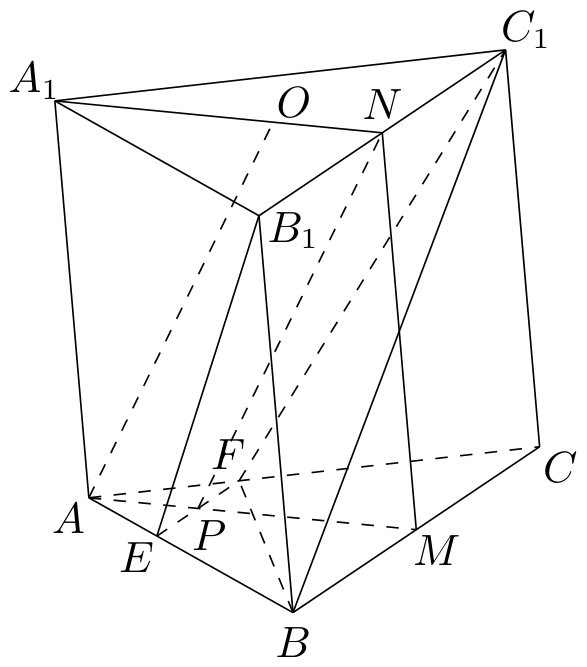
\includegraphics[width=5.6cm]{GaoKao/images/2020/national_paper_2_liberal/q20_fig1.png}
\par}
        
        \begin{enumerate}[label=(\arabic*)]
            \item 证明: $AA_1\parallel MN$, 且平面$A_1AMN\perp$平面$EB_1C_1F$;
            \item 设$O$为$\triangle A_1B_1C_1$的中心, 若$AO=AB=6$, $AO\parallel$平面$EB_1C_1F$, 且$\angle MPN=\dfrac{\pi}{3}$, 求四棱锥$B-EB_1C_1F$的体积.
        \end{enumerate}
        
        \item 已知函数$f(x)=2\ln x+1$.
        \begin{enumerate}[label=(\arabic*)]
            \item 若$f(x)\leqslant 2x+c$, 求$c$的取值范围;
            \item 设$a>0$时, 讨论函数$g(x)=\dfrac{f(x)-f(a)}{x-a}$的单调性.
        \end{enumerate}
        
        \item 已知曲线$C_1,C_2$的参数方程分别为$C_1:\begin{cases}x=4\cos^{2}\theta,\\y=4\sin^{2}\theta;\end{cases}$ ($\theta$为参数), $C_2:\begin{cases}x=t+\dfrac{1}{t},\\[6pt]y=t-\dfrac{1}{t};\end{cases}$ ($t$为参数).
        \begin{enumerate}[label=(\arabic*)]
            \item 将$C_1,C_2$的参数方程化为普通方程;
            \item 以坐标原点为极点, $x$轴正半轴为极轴建立极坐标系. 设$C_1,C_2$的交点为$P$, 求圆心在极轴上, 且经过极点和$P$的圆的极坐标方程.
        \end{enumerate}
        
        \item 已知函数$f(x)=|x-a^{2}|+|x-2a+1|$.
        \begin{enumerate}[label=(\arabic*)]
            \item 当$a=2$时, 求不等式$f(x)\geqslant 4$的解集;
            \item 若$f(x)\geqslant 4$, 求$a$的取值范围.
        \end{enumerate}
        
    \end{enumerate}
\end{description}
\clearpage


\subsection{2020年全国III卷（理）}\label{gk:2020年全国III卷（理）}

\begin{description}
    \item[一、选择题]
    \begin{enumerate}[leftmargin=5pt]
        \item 已知集合$A=\{(x,y)\mid x,y\in\mathbb{N}^{*},\;y\geqslant x\}$, $B=\{(x,y)\mid x+y=8\}$, 则$A\cap B$中元素的个数为 (\qquad)
        
        {\centering\begin{tabular*}{\linewidth}{@{}@{\extracolsep{\fill}}llll@{}}
            \(\text{A. } 2\)  & \(\text{B. } 3\)  & \(\text{C. } 4\)  & \(\text{D. } 6\)
        \end{tabular*}\par}
        
        \item 复数$\dfrac{1}{1-3\i}$的虚部是 (\qquad)
        
        {\centering\begin{tabular*}{\linewidth}{@{}@{\extracolsep{\fill}}llll@{}}
            \(\text{A. } -\dfrac{3}{10}\)  & \(\text{B. } -\dfrac{1}{10}\)  & \(\text{C. } \dfrac{1}{10}\)  & \(\text{D. } \dfrac{3}{10}\)
        \end{tabular*}\par}
        
        \item 在一组样本数据中, $1,2,3,4$出现的频率分别为$p_1,p_2,p_3,p_4$, 且$\displaystyle\sum_{i=1}^{4}p_i=1$, 则下面四种情形中, 对应样本的标准差最大的一组是 (\qquad)
        
        {\centering\begin{tabular*}{\linewidth}{@{}@{\extracolsep{\fill}}llll@{}}
            \(\text{A. } p_1=p_4=0.1,\;p_2=p_3=0.4\)  & \(\text{B. } p_1=p_4=0.4,\;p_2=p_3=0.1\)  \\
            \(\text{C. } p_1=p_4=0.2,\;p_2=p_3=0.3\)  & \(\text{D. } p_1=p_4=0.3,\;p_2=p_3=0.2\)
        \end{tabular*}\par}
        
        \item Logistic模型是常用数学模型之一, 可应用于流行病学领域. 有学者根据公布数据建立了某地区新冠肺炎累计确诊病例数$I(t)$ ($t$的单位: 天)的Logistic模型: $I(t)=\dfrac{K}{1+\mathrm{e}^{-0.23(t-53)}}$, 其中$K$为最大确诊病例数. 当$I(t^{*})=0.95K$时, 标志着已初步遏制疫情, 则$t^{*}$约为$(\ln 19\approx 3)$ (\qquad)
        
        {\centering\begin{tabular*}{\linewidth}{@{}@{\extracolsep{\fill}}llll@{}}
            \(\text{A. } 60\)  & \(\text{B. } 63\)  & \(\text{C. } 66\)  & \(\text{D. } 69\)
        \end{tabular*}\par}
        
        \item 设$O$为坐标原点, 直线$x=2$与抛物线$C:y^{2}=2px$ $(p>0)$交于$D,E$两点. 若$OD\perp OE$, 则$C$的焦点坐标为 (\qquad)
        
        {\centering\begin{tabular*}{\linewidth}{@{}@{\extracolsep{\fill}}llll@{}}
            \(\text{A. } \bigl(\dfrac{1}{4},0\bigr)\)  & \(\text{B. } \bigl(\dfrac{1}{2},0\bigr)\)  & \(\text{C. } (1,0)\)  & \(\text{D. } (2,0)\)
        \end{tabular*}\par}
        
        \item 已知向量$\bm{a},\bm{b}$满足$|\bm{a}|=5$, $|\bm{b}|=6$, $\bm{a}\cdot\bm{b}=-6$, 则$\cos\langle\bm{a},\bm{a}+\bm{b}\rangle=$ (\qquad)
        
        {\centering\begin{tabular*}{\linewidth}{@{}@{\extracolsep{\fill}}llll@{}}
            \(\text{A. } -\dfrac{31}{35}\)  & \(\text{B. } -\dfrac{19}{35}\)  & \(\text{C. } \dfrac{17}{35}\)  & \(\text{D. } \dfrac{19}{35}\)
        \end{tabular*}\par}
        
        \item 在$\triangle ABC$中, $\cos C=\dfrac{2}{3}$, $AC=4$, $BC=3$, 则$\cos B=$ (\qquad)
        
        {\centering\begin{tabular*}{\linewidth}{@{}@{\extracolsep{\fill}}llll@{}}
            \(\text{A. } \dfrac{1}{9}\)  & \(\text{B. } \dfrac{1}{3}\)  & \(\text{C. } \dfrac{1}{2}\)  & \(\text{D. } \dfrac{2}{3}\)
        \end{tabular*}\par}
        
        \item 下图为某几何体的三视图, 则该几何体的表面积是 (\qquad)
        
        {\centering
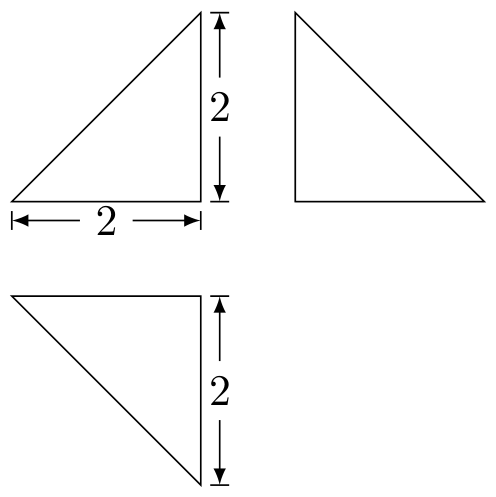
\includegraphics[width=4.9cm]{GaoKao/images/2020/national_paper_3_science/q8_fig1.png}
\par}
        
        {\centering\begin{tabular*}{\linewidth}{@{}@{\extracolsep{\fill}}llll@{}}
            \(\text{A. } 6+4\sqrt{2}\)  & \(\text{B. } 4+4\sqrt{2}\)  & \(\text{C. } 6+2\sqrt{3}\)  & \(\text{D. } 4+2\sqrt{3}\)
        \end{tabular*}\par}
        
        \item 已知$2\tan\theta-\tan\bigl(\theta+\dfrac{\pi}{4}\bigr)=7$, 则$\tan\theta=$ (\qquad)
        
        {\centering\begin{tabular*}{\linewidth}{@{}@{\extracolsep{\fill}}llll@{}}
            \(\text{A. } -2\)  & \(\text{B. } -1\)  & \(\text{C. } 1\)  & \(\text{D. } 2\)
        \end{tabular*}\par}
        
        \item 若直线$l$与曲线$y=\sqrt{x}$和$x^{2}+y^{2}=\dfrac{1}{5}$都相切, 则$l$的方程为 (\qquad)
        
        {\centering\begin{tabular*}{\linewidth}{@{}@{\extracolsep{\fill}}llll@{}}
            \(\text{A. } y=2x+1\)  & \(\text{B. } y=2x+\dfrac{1}{2}\)  & \(\text{C. } y=\dfrac{1}{2}x+1\)  & \(\text{D. } y=\dfrac{1}{2}x+\dfrac{1}{2}\)
        \end{tabular*}\par}
        
        \item 设双曲线$C:\dfrac{x^{2}}{a^{2}}-\dfrac{y^{2}}{b^{2}}=1$ $(a>0,b>0)$的左、右焦点分别为$F_1,F_2$, 离心率为$\sqrt{5}$. $P$是$C$上一点, 且$F_1P\perp F_2P$. 若$\triangle PF_1F_2$的面积为$4$, 则$a=$ (\qquad)
        
        {\centering\begin{tabular*}{\linewidth}{@{}@{\extracolsep{\fill}}llll@{}}
            \(\text{A. } 1\)  & \(\text{B. } 2\)  & \(\text{C. } 4\)  & \(\text{D. } 8\)
        \end{tabular*}\par}
        
        \item 已知$5^{5}<8^{4}$, $13^{4}<8^{5}$. 设$a=\log_{5}3$, $b=\log_{8}5$, $c=\log_{13}8$, 则 (\qquad)
        
        {\centering\begin{tabular*}{\linewidth}{@{}@{\extracolsep{\fill}}llll@{}}
            \(\text{A. } a<b<c\)  & \(\text{B. } b<a<c\)  & \(\text{C. } b<c<a\)  & \(\text{D. } c<a<b\)
        \end{tabular*}\par}
        
    \end{enumerate}
    
    \item[二、填空题]
    \begin{enumerate}[leftmargin=5pt]
      \addtocounter{enumi}{+12}
        \item 若$x,y$满足约束条件$\begin{cases}x+y\geqslant 0,\\2x-y\geqslant 0,\\x\leqslant 1,\end{cases}$ 则$z=3x+2y$的最大值为 \rule[-0.3ex]{3em}{0.4pt}.
        \item $\bigl(x^{2}+\dfrac{2}{x}\bigr)^{6}$的展开式中常数项是 \rule[-0.3ex]{3em}{0.4pt}. (用数字作答)
        \item 已知圆锥的底面半径为$1$, 母线长为$3$, 则该圆锥内半径最大的球的体积为 \rule[-0.3ex]{3em}{0.4pt}.
        \item 关于函数$f(x)=\sin x+\dfrac{1}{\sin x}$有如下四个命题:\\
        \ding{172} $f(x)$的图像关于$y$轴对称;\\
        \ding{173} $f(x)$的图像关于原点对称;\\
        \ding{174} $f(x)$的图像关于直线$x=\dfrac{\pi}{2}$对称;\\
        \ding{175} $f(x)$的最小值为$2$.\\
        其中所有真命题的序号是 \rule[-0.3ex]{3em}{0.4pt}.
    \end{enumerate}
    
    \item[三、解答题]
    \begin{enumerate}[leftmargin=5pt]
      \addtocounter{enumi}{+16}
        \item 设数列$\{a_n\}$满足$a_1=3$, $a_{n+1}=3a_n-4n$.
        \begin{enumerate}[label=(\arabic*)]
            \item 计算$a_2,a_3$, 猜想$\{a_n\}$的通项公式并加以证明;
            \item 求数列$\{2^{n}a_n\}$的前$n$项和$S_n$.
        \end{enumerate}

        \item 某学生兴趣小组随机调查了某市$100$天中每天的空气质量等级和当天到某公园锻炼的人次, 整理数据得到下表(单位: 天):
        
        \begin{center}
        \begin{tabular}{|c|c|c|c|}
        \hline
        \makebox[3cm]{锻炼人次} & $[0,200]$ & $(200,400]$ & $(400,600]$ \\
        \makebox[3cm]{空气质量等级} & & & \\
        \hline
        $1$(优) & $2$ & $16$ & $25$ \\
        \hline
        $2$(良) & $5$ & $10$ & $12$ \\
        \hline
        $3$(轻度污染) & $6$ & $7$ & $8$ \\
        \hline
        $4$(中度污染) & $7$ & $2$ & $0$ \\
        \hline
        \end{tabular}
        \end{center}
        
        \begin{enumerate}[label=(\arabic*)]
            \item 分别估计该市一天的空气质量等级为$1,2,3,4$的概率;
            \item 求一天中到该公园锻炼的平均人次的估计值(同一组中的数据用该组区间的中点值为代表);
            \item 若某天的空气质量等级为$1$或$2$, 则称这天"空气质量好"; 若某天的空气质量等级为$3$或$4$, 则称这天"空气质量不好". 根据所给数据, 完成下面的$2\times 2$列联表, 并根据列联表, 判断是否有$95\%$的把握认为一天中到该公园锻炼的人次与该市当天的空气质量有关?
        \end{enumerate}
        
        \begin{center}
        \begin{tabular}{|c|c|c|}
        \hline
        & 人次$\leqslant 400$ & 人次$>400$ \\
        \hline
        空气质量好 & & \\
        \hline
        空气质量不好 & & \\
        \hline
        \end{tabular}
        \end{center}
        
        附: $K^{2}=\dfrac{n(ad-bc)^{2}}{(a+b)(c+d)(a+c)(b+d)}$,
        
        \begin{center}
        \begin{tabular}{|c|c|c|c|}
        \hline
        $P(K^{2}\geqslant k)$ & $0.050$ & $0.010$ & $0.001$ \\
        \hline
        $k$ & $3.841$ & $6.635$ & $10.828$ \\
        \hline
        \end{tabular}
        \end{center}
        
        \item 如图, 在长方体$ABCD-A_1B_1C_1D_1$中, 点$E,F$分别在棱$DD_1,BB_1$上, 且$2DE=ED_1$, $BF=2FB_1$.
        
        {\centering
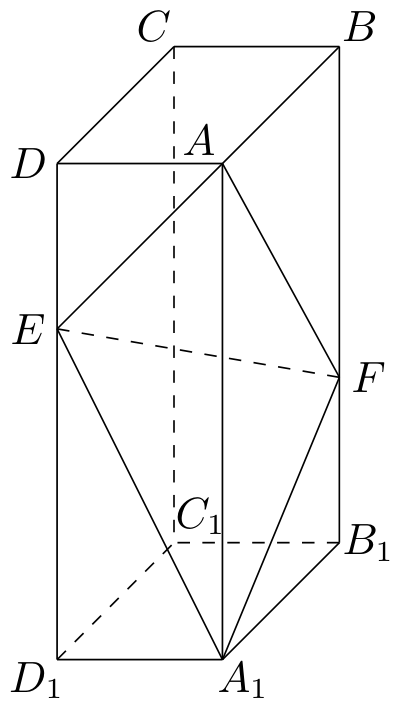
\includegraphics[width=4.1cm]{GaoKao/images/2020/national_paper_3_science/q19_fig1.png}
\par}
        
        \begin{enumerate}[label=(\arabic*)]
            \item 证明: 点$C_1$在平面$AEF$内;
            \item 若$AB=2$, $AD=1$, $AA_1=3$, 求二面角$A-EF-A_1$的正弦值.
        \end{enumerate}
        
        \item 已知椭圆$C:\dfrac{x^{2}}{25}+\dfrac{y^{2}}{m^{2}}=1$ $(0<m<5)$的离心率为$\dfrac{\sqrt{15}}{4}$, $A,B$分别为$C$的左、右顶点.
        \begin{enumerate}[label=(\arabic*)]
            \item 求$C$的方程;
            \item 若点$P$在$C$上, 点$Q$在直线$x=6$上, 且$|BP|=|BQ|$, $BP\perp BQ$, 求$\triangle APQ$的面积.
        \end{enumerate}
        
        \item 设函数$f(x)=x^{3}+bx+c$, 曲线$y=f(x)$在点$\bigl(\dfrac{1}{2},f\bigl(\dfrac{1}{2}\bigr)\bigr)$处的切线与$y$轴垂直.
        \begin{enumerate}[label=(\arabic*)]
            \item 求$b$;
            \item 若$f(x)$有一个绝对值不大于$1$的零点, 证明: $f(x)$所有零点的绝对值都不大于$1$.
        \end{enumerate}
        
        \item 在直角坐标系$xOy$中, 曲线$C$的参数方程为$\begin{cases}x=2-t-t^{2},\\y=2-3t+t^{2};\end{cases}$ ($t$为参数且$t\neq 1$), $C$与坐标轴交于$A,B$两点.
        \begin{enumerate}[label=(\arabic*)]
            \item 求$|AB|$;
            \item 以坐标原点为极点, $x$轴正半轴为极轴建立极坐标系, 求直线$AB$的极坐标方程.
        \end{enumerate}
        
        \item 设$a,b,c\in\mathbb{R}$, $a+b+c=0$, $abc=1$.
        \begin{enumerate}[label=(\arabic*)]
            \item 证明: $ab+bc+ca<0$;
            \item 用$\max\{a,b,c\}$表示$a,b,c$中的最大值, 证明: $\max\{a,b,c\}\geqslant\sqrt[3]{4}$.
        \end{enumerate}
        
    \end{enumerate}
\end{description}
\clearpage


\subsection{2020年全国III卷（文）}\label{gk:2020年全国III卷（文）}

\begin{description}
    \item[一、选择题]
    \begin{enumerate}[leftmargin=5pt]
        \item 已知集合$A=\{1,2,3,5,7,11\}$, $B=\{x\mid 3<x<15\}$, 则$A\cap B$中元素的个数为 (\qquad)
        
        {\centering\begin{tabular*}{\linewidth}{@{}@{\extracolsep{\fill}}llll@{}}
            \(\text{A. } 2\)  & \(\text{B. } 3\)  & \(\text{C. } 4\)  & \(\text{D. } 5\)
        \end{tabular*}\par}
        
        \item 若$\overline{z}(1+\i)=1-\i$, 则$z=$ (\qquad)
        
        {\centering\begin{tabular*}{\linewidth}{@{}@{\extracolsep{\fill}}llll@{}}
            \(\text{A. } 1-\i\)  & \(\text{B. } 1+\i\)  & \(\text{C. } -\i\)  & \(\text{D. } \i\)
        \end{tabular*}\par}
        
        \item 设一组样本数据$x_1,x_2,\cdots,x_n$的方差为$0.01$, 则数据$10x_1,10x_2,\cdots,10x_n$的方差为 (\qquad)
        
        {\centering\begin{tabular*}{\linewidth}{@{}@{\extracolsep{\fill}}llll@{}}
            \(\text{A. } 0.01\)  & \(\text{B. } 0.1\)  & \(\text{C. } 1\)  & \(\text{D. } 10\)
        \end{tabular*}\par}
        
        \item Logistic模型是常用数学模型之一, 可应用于流行病学领域. 有学者根据公布数据建立了某地区新冠肺炎累计确诊病例数$I(t)$ ($t$的单位: 天)的Logistic模型: $I(t)=\dfrac{K}{1+\mathrm{e}^{-0.23(t-53)}}$, 其中$K$为最大确诊病例数. 当$I(t^{*})=0.95K$时, 标志着已初步遏制疫情, 则$t^{*}$约为$(\ln 19\approx 3)$ (\qquad)
        
        {\centering\begin{tabular*}{\linewidth}{@{}@{\extracolsep{\fill}}llll@{}}
            \(\text{A. } 60\)  & \(\text{B. } 63\)  & \(\text{C. } 66\)  & \(\text{D. } 69\)
        \end{tabular*}\par}
        
        \item 已知$\sin\theta+\sin\bigl(\theta+\dfrac{\pi}{3}\bigr)=1$, 则$\sin\bigl(\theta+\dfrac{\pi}{6}\bigr)=$ (\qquad)
        
        {\centering\begin{tabular*}{\linewidth}{@{}@{\extracolsep{\fill}}llll@{}}
            \(\text{A. } \dfrac{1}{2}\)  & \(\text{B. } \dfrac{\sqrt{3}}{3}\)  & \(\text{C. } \dfrac{2}{3}\)  & \(\text{D. } \dfrac{\sqrt{2}}{2}\)
        \end{tabular*}\par}
        
        \item 在平面内, $A,B$是两个定点, $C$是动点. 若$\overrightarrow{AC}\cdot\overrightarrow{BC}=1$, 则点$C$的轨迹为 (\qquad)
        
        {\centering\begin{tabular*}{\linewidth}{@{}@{\extracolsep{\fill}}llll@{}}
            \(\text{A. } \text{圆}\)  & \(\text{B. } \text{椭圆}\)  & \(\text{C. } \text{抛物线}\)  & \(\text{D. } \text{直线}\)
        \end{tabular*}\par}
        
        \item 设$O$为坐标原点, 直线$x=2$与抛物线$C:y^{2}=2px$ $(p>0)$交于$D,E$两点. 若$OD\perp OE$, 则$C$的焦点坐标为 (\qquad)
        
        {\centering\begin{tabular*}{\linewidth}{@{}@{\extracolsep{\fill}}llll@{}}
            \(\text{A. } \bigl(\dfrac{1}{4},0\bigr)\)  & \(\text{B. } \bigl(\dfrac{1}{2},0\bigr)\)  & \(\text{C. } (1,0)\)  & \(\text{D. } (2,0)\)
        \end{tabular*}\par}
        
        \item 点$(0,-1)$到直线$y=k(x+1)$距离的最大值为 (\qquad)
        
        {\centering\begin{tabular*}{\linewidth}{@{}@{\extracolsep{\fill}}llll@{}}
            \(\text{A. } 1\)  & \(\text{B. } \sqrt{2}\)  & \(\text{C. } \sqrt{3}\)  & \(\text{D. } 2\)
        \end{tabular*}\par}
        
        \item 下图为某几何体的三视图, 则该几何体的表面积是 (\qquad)
        
        {\centering
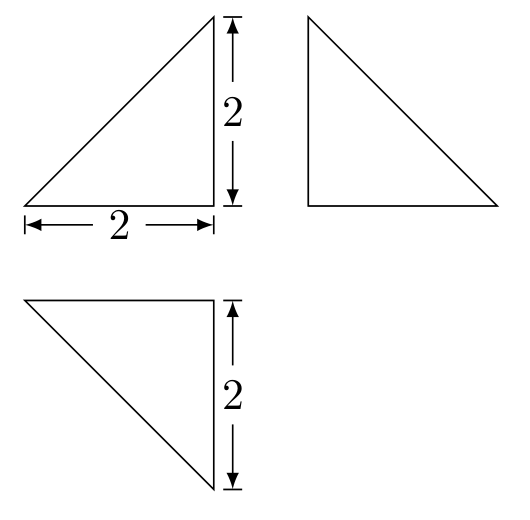
\includegraphics[width=0.65\linewidth]{GaoKao/images/2020/national_paper_3_liberal/q9_fig1.png}
\par}
        
        {\centering\begin{tabular*}{\linewidth}{@{}@{\extracolsep{\fill}}llll@{}}
            \(\text{A. } 6+4\sqrt{2}\)  & \(\text{B. } 4+4\sqrt{2}\)  & \(\text{C. } 6+2\sqrt{3}\)  & \(\text{D. } 4+2\sqrt{3}\)
        \end{tabular*}\par}
        
        \item 设$a=\log_{3}2$, $b=\log_{5}3$, $c=\dfrac{2}{3}$, 则 (\qquad)
        
        {\centering\begin{tabular*}{\linewidth}{@{}@{\extracolsep{\fill}}llll@{}}
            \(\text{A. } a<c<b\)  & \(\text{B. } a<b<c\)  & \(\text{C. } b<c<a\)  & \(\text{D. } c<a<b\)
        \end{tabular*}\par}
        
        \item 在$\triangle ABC$中, $\cos C=\dfrac{2}{3}$, $AC=4$, $BC=3$, 则$\tan B=$ (\qquad)
        
        {\centering\begin{tabular*}{\linewidth}{@{}@{\extracolsep{\fill}}llll@{}}
            \(\text{A. } \sqrt{5}\)  & \(\text{B. } 2\sqrt{5}\)  & \(\text{C. } 4\sqrt{5}\)  & \(\text{D. } 8\sqrt{5}\)
        \end{tabular*}\par}
        
        \item 已知函数$f(x)=\sin x+\dfrac{1}{\sin x}$, 则 (\qquad)
        
        {\centering\begin{tabular*}{\linewidth}{@{}@{\extracolsep{\fill}}llll@{}}
            \(\text{A. } f(x)\text{的最小值为}2\)  & \(\text{B. } f(x)\text{的图像关于}y\text{轴对称}\)  \\
            \(\text{C. } f(x)\text{的图像关于直线}x=\pi\text{对称}\)  & \(\text{D. } f(x)\text{的图像关于直线}x=\dfrac{\pi}{2}\text{对称}\)
        \end{tabular*}\par}
        
    \end{enumerate}
    
    \item[二、填空题]
    \begin{enumerate}[leftmargin=5pt]
      \addtocounter{enumi}{+12}
        \item 若$x,y$满足约束条件$\begin{cases}x+y\geqslant 0,\\2x-y\geqslant 0,\\x\leqslant 1,\end{cases}$ 则$z=3x+2y$的最大值为 \rule[-0.3ex]{3em}{0.4pt}.
        \item 设双曲线$C:\dfrac{x^{2}}{a^{2}}-\dfrac{y^{2}}{b^{2}}=1$ $(a>0,b>0)$的一条渐近线为$y=\sqrt{2}x$, 则$C$的离心率为 \rule[-0.3ex]{3em}{0.4pt}.
        \item 设函数$f(x)=\dfrac{\mathrm{e}^{x}}{x+a}$. 若$f'(1)=\dfrac{\mathrm{e}}{4}$, 则$a=$ \rule[-0.3ex]{3em}{0.4pt}.
        \item 已知圆锥的底面半径为$1$, 母线长为$3$, 则该圆锥内半径最大的球的体积为 \rule[-0.3ex]{3em}{0.4pt}.
    \end{enumerate}
    
    \item[三、解答题]
    \begin{enumerate}[leftmargin=5pt]
      \addtocounter{enumi}{+16}
        \item 设等比数列$\{a_n\}$满足$a_1+a_2=4$, $a_3-a_1=8$.
        \begin{enumerate}[label=(\arabic*)]
            \item 求$\{a_n\}$的通项公式;
            \item 设$S_n$为数列$\{\log_{3}a_n\}$的前$n$项和. 若$S_m+S_{m+1}=S_{m+3}$, 求$m$.
        \end{enumerate}

        \item 某学生兴趣小组随机调查了某市$100$天中每天的空气质量等级和当天到某公园锻炼的人次, 整理数据得到下表(单位: 天):
        
        \begin{center}
        \begin{tabular}{|c|c|c|c|}
        \hline
        \makebox[3cm]{锻炼人次} & $[0,200]$ & $(200,400]$ & $(400,600]$ \\
        \makebox[3cm]{空气质量等级} & & & \\
        \hline
        $1$(优) & $2$ & $16$ & $25$ \\
        \hline
        $2$(良) & $5$ & $10$ & $12$ \\
        \hline
        $3$(轻度污染) & $6$ & $7$ & $8$ \\
        \hline
        $4$(中度污染) & $7$ & $2$ & $0$ \\
        \hline
        \end{tabular}
        \end{center}
        
        \begin{enumerate}[label=(\arabic*)]
            \item 分别估计该市一天的空气质量等级为$1,2,3,4$的概率;
            \item 求一天中到该公园锻炼的平均人次的估计值(同一组中的数据用该组区间的中点值为代表);
            \item 若某天的空气质量等级为$1$或$2$, 则称这天"空气质量好"; 若某天的空气质量等级为$3$或$4$, 则称这天"空气质量不好". 根据所给数据, 完成下面的$2\times 2$列联表, 并根据列联表, 判断是否有$95\%$的把握认为一天中到该公园锻炼的人次与该市当天的空气质量有关?
        \end{enumerate}
        
        \begin{center}
        \begin{tabular}{|c|c|c|}
        \hline
        & 人次$\leqslant 400$ & 人次$>400$ \\
        \hline
        空气质量好 & & \\
        \hline
        空气质量不好 & & \\
        \hline
        \end{tabular}
        \end{center}
        
        附: $K^{2}=\dfrac{n(ad-bc)^{2}}{(a+b)(c+d)(a+c)(b+d)}$,
        
        \begin{center}
        \begin{tabular}{|c|c|c|c|}
        \hline
        $P(K^{2}\geqslant k)$ & $0.050$ & $0.010$ & $0.001$ \\
        \hline
        $k$ & $3.841$ & $6.635$ & $10.828$ \\
        \hline
        \end{tabular}
        \end{center}
        
        \item 如图, 在长方体$ABCD-A_1B_1C_1D_1$中, 点$E,F$分别在棱$DD_1,BB_1$上, 且$2DE=ED_1$, $BF=2FB_1$. 证明:
        
        {\centering
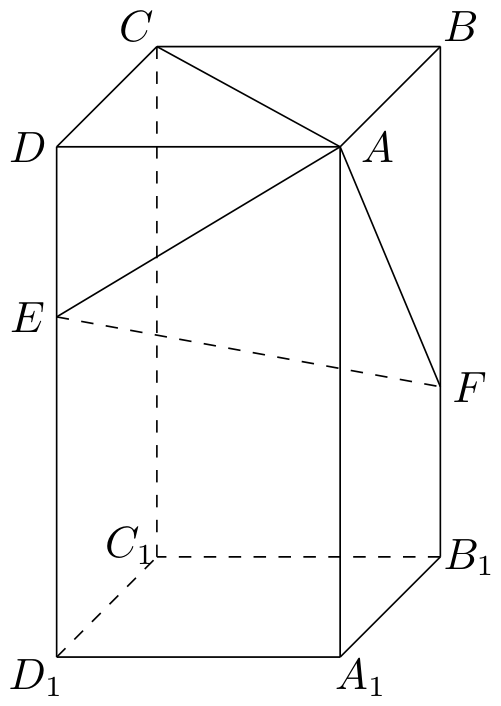
\includegraphics[width=4.8cm]{GaoKao/images/2020/national_paper_3_liberal/q19_fig1.png}
\par}
        
        \begin{enumerate}[label=(\arabic*)]
            \item 当$AB=BC$时, $EF\perp AC$;
            \item 点$C_1$在平面$AEF$内.
        \end{enumerate}
        
        \item 已知函数$f(x)=x^{3}-kx+k^{2}$.
        \begin{enumerate}[label=(\arabic*)]
            \item 讨论$f(x)$的单调性;
            \item 若$f(x)$有三个零点, 求$k$的取值范围.
        \end{enumerate}
        
        \item 已知椭圆$C:\dfrac{x^{2}}{25}+\dfrac{y^{2}}{m^{2}}=1$ $(0<m<5)$的离心率为$\dfrac{\sqrt{15}}{4}$, $A,B$分别为$C$的左、右顶点.
        \begin{enumerate}[label=(\arabic*)]
            \item 求$C$的方程;
            \item 若点$P$在$C$上, 点$Q$在直线$x=6$上, 且$|BP|=|BQ|$, $BP\perp BQ$, 求$\triangle APQ$的面积.
        \end{enumerate}
        
        \item 在直角坐标系$xOy$中, 曲线$C$的参数方程为$\begin{cases}x=2-t-t^{2},\\y=2-3t+t^{2};\end{cases}$ ($t$为参数且$t\neq 1$), $C$与坐标轴交于$A,B$两点.
        \begin{enumerate}[label=(\arabic*)]
            \item 求$|AB|$;
            \item 以坐标原点为极点, $x$轴正半轴为极轴建立极坐标系, 求直线$AB$的极坐标方程.
        \end{enumerate}
        
        \item 设$a,b,c\in\mathbb{R}$, $a+b+c=0$, $abc=1$.
        \begin{enumerate}[label=(\arabic*)]
            \item 证明: $ab+bc+ca<0$;
            \item 用$\max\{a,b,c\}$表示$a,b,c$中的最大值, 证明: $\max\{a,b,c\}\geqslant\sqrt[3]{4}$.
        \end{enumerate}
        
    \end{enumerate}
\end{description}
\clearpage


\subsection{2020年新高考I卷}\label{gk:2020年新高考I卷}

\begin{description}
    \item[一、单选题]
    \begin{enumerate}[leftmargin=5pt]
        \item 设集合$A=\{x\mid 1\leqslant x\leqslant 3\}$，$B=\{x\mid 2<x<4\}$，则$A\cup B=$（\quad）
        {\centering\begin{tabular*}{\linewidth}{@{}@{\extracolsep{\fill}}llll@{}}
            $\text{A. }\{x\mid 2<x\leqslant 3\}$  & $\text{B. }\{x\mid 2\leqslant x\leqslant 3\}$  & $\text{C. }\{x\mid 1\leqslant x<4\}$  & $\text{D. }\{x\mid 1<x<4\}$
        \end{tabular*}\par}
        \item $\dfrac{2-\i}{1+2\i}=$（\quad）
        {\centering\begin{tabular*}{\linewidth}{@{}@{\extracolsep{\fill}}llll@{}}
            $\text{A. }1$  & $\text{B. }-1$  & $\text{C. }\i$  & $\text{D. }-\i$
        \end{tabular*}\par}
        \item $6$名同学到甲、乙、丙三个场馆做志愿者，每名同学只去$1$个场馆，甲场馆安排$1$名，乙场馆安排$2$名，丙场馆安排$3$名，则不同的安排方法共有（\quad）
        {\centering\begin{tabular*}{\linewidth}{@{}@{\extracolsep{\fill}}llll@{}}
            $\text{A. }120$种  & $\text{B. }90$种  & $\text{C. }60$种  & $\text{D. }30$种
        \end{tabular*}\par}
        \item 日晷是中国古代用来测定时间的仪器，利用与晷面垂直的晷针投射到晷面的影子来测定时间．把地球看成一个球（球心记为$O$），地球上一点$A$的纬度是指$OA$与地球赤道所在平面所成角，点$A$处的水平面是指过点$A$且与$OA$垂直的平面．在点$A$处放置一个日晷，若晷面与赤道所在平面平行，点$A$处的纬度为北纬$40^{\circ}$，则晷针与点$A$处的水平面所成角为（\quad）
        {\centering\begin{tabular*}{\linewidth}{@{}@{\extracolsep{\fill}}llll@{}}
            $\text{A. }20^{\circ}$  & $\text{B. }40^{\circ}$  & $\text{C. }50^{\circ}$  & $\text{D. }90^{\circ}$
        \end{tabular*}\par}
        \item 某中学的学生积极参加体育锻炼，其中有$96\%$的学生喜欢足球或游泳，$60\%$的学生喜欢足球，$82\%$的学生喜欢游泳，则该中学既喜欢足球又喜欢游泳的学生数占该校学生总数的比例是（\quad）
        {\centering\begin{tabular*}{\linewidth}{@{}@{\extracolsep{\fill}}llll@{}}
            $\text{A. }62\%$  & $\text{B. }56\%$  & $\text{C. }46\%$  & $\text{D. }42\%$
        \end{tabular*}\par}        \item 基本再生数$R_{0}$与世代间隔$T$是新冠肺炎的流行病学基本参数．基本再生数指一个感染者传染的平均人数，世代间隔指相邻两代间传染所需的平均时间．在新冠肺炎疫情初始阶段，可以用指数模型：$I(t)=\mathrm{e}^{rt}$描述累计感染病例数$I(t)$随时间$t$（单位：天）的变化规律，指数增长率$r$与$R_{0},T$近似满足$R_{0}=1+rT$．有学者基于已有数据估计出$R_{0}=3.28$，$T=6$．据此，在新冠肺炎疫情初始阶段，累计感染病例数增加$1$倍需要的时间约为$(\ln 2\approx 0.69)$（\quad）
        {\centering\begin{tabular*}{\linewidth}{@{}@{\extracolsep{\fill}}llll@{}}
            $\text{A. }1.2$天  & $\text{B. }1.8$天  & $\text{C. }2.5$天  & $\text{D. }3.5$天
        \end{tabular*}\par}
        \item 已知$P$是边长为$2$的正六边形$ABCDEF$内的一点，则$\overrightarrow{AP}\cdot\overrightarrow{AB}$的取值范围是（\quad）
        {\centering\begin{tabular*}{\linewidth}{@{}@{\extracolsep{\fill}}llll@{}}
            $\text{A. }(-2,6)$  & $\text{B. }(-6,2)$  & $\text{C. }(-2,4)$  & $\text{D. }(-4,6)$
        \end{tabular*}\par}
        \item 若定义在$\mathbb{R}$的奇函数$f(x)$在$(-\infty,0)$单调递减，且$f(2)=0$，则满足$xf(x-1)\geqslant 0$的$x$的取值范围是（\quad）
        {\centering\begin{tabular*}{\linewidth}{@{}@{\extracolsep{\fill}}llll@{}}
            $\text{A. }[-1,1]\cup[3,+\infty)$  & $\text{B. }[-3,-1]\cup[0,1]$  & $\text{C. }[-1,0]\cup[1,+\infty)$  & $\text{D. }[-1,0]\cup[1,3]$
        \end{tabular*}\par}
    \end{enumerate}
    \item[二、多选题]
    \begin{enumerate}[leftmargin=5pt]
      \addtocounter{enumi}{+8}
        \item 已知曲线$C:mx^{2}+ny^{2}=1$（\quad）
        \begin{enumerate}[label=\Alph*.]
            \item 若$m>n>0$，则$C$是椭圆，其焦点在$y$轴上
            \item 若$m=n>0$，则$C$是圆，其半径为$\sqrt{n}$
            \item 若$mn<0$，则$C$是双曲线，其渐近线方程为$y=\pm\sqrt{-\dfrac{m}{n}}x$
            \item 若$m=0,n>0$，则$C$是两条直线
        \end{enumerate}        \item 下图是函数$y=\sin(\omega x+\varphi)$的部分图象，则$\sin(\omega x+\varphi)=$（\quad）
        {\centering
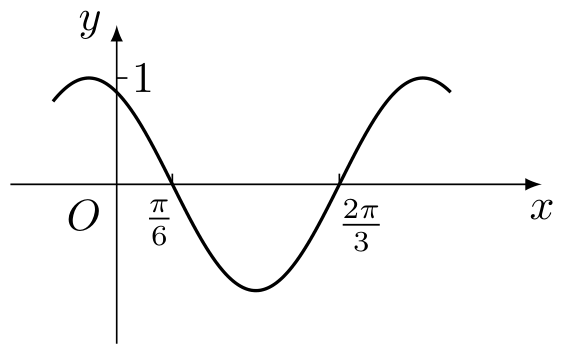
\includegraphics[width=5.7cm]{GaoKao/images/2020/new_gaokao_paper_1/q10_fig1.png}
\par}
        \begin{enumerate}[label=\Alph*.]
            \item $\sin\bigl(x+\frac{\pi}{3}\bigr)$
            \item $\sin\bigl(\frac{\pi}{3}-2x\bigr)$
            \item $\cos\bigl(2x+\frac{\pi}{6}\bigr)$
            \item $\cos\bigl(\frac{5\pi}{6}-2x\bigr)$
        \end{enumerate}
        \item 已知$a>0$，$b>0$，且$a+b=1$，则（\quad）
        \begin{enumerate}[label=\Alph*.]
            \item $a^{2}+b^{2}\geqslant\dfrac{1}{2}$
            \item $2^{a-b}>\dfrac{1}{2}$
            \item $\log_{2}a+\log_{2}b\geqslant -2$
            \item $\sqrt{a}+\sqrt{b}\leqslant\sqrt{2}$
        \end{enumerate}
        \item 信息熵是信息论中的一个重要概念．设随机变量$X$所有可能的取值为$1,2,\cdots,n$，且$P(X=i)=p_{i}>0$（$i=1,2,\cdots,n$），$\sum\limits_{i=1}^{n}p_{i}=1$，定义$X$的信息熵$H(X)=-\sum\limits_{i=1}^{n}p_{i}\log_{2}p_{i}$．（\quad）
        \begin{enumerate}[label=\Alph*.]
            \item 若$n=1$，则$H(X)=0$
            \item 若$n=2$，则$H(X)$随着$p_{1}$的增大而增大
            \item 若$p_{i}=\dfrac{1}{n}$（$i=1,2,\cdots,n$），则$H(X)$随着$n$的增大而增大
            \item 若$n=2m$，随机变量$Y$所有可能的取值为$1,2,\cdots,m$，且$P(Y=j)=p_{j}+p_{2m+1-j}$（$j=1,2,\cdots,m$），则$H(X)\leqslant H(Y)$
        \end{enumerate}
    \end{enumerate}
    \item[三、填空题]
    \begin{enumerate}[leftmargin=5pt]
      \addtocounter{enumi}{+12}
        \item 斜率为$\sqrt{3}$的直线过抛物线$C:y^{2}=4x$的焦点，且与$C$交于$A,B$两点，则$|AB|=\rule[-0.3ex]{3em}{0.4pt}$．
        \item 将数列$\{2n-1\}$与$\{3n-2\}$的公共项从小到大排列得到数列$\{a_{n}\}$，则$\{a_{n}\}$的前$n$项和为\rule[-0.3ex]{6em}{0.4pt}．        \item 某中学开展劳动实习，学生加工制作零件，零件的截面如图所示．$O$为圆孔及轮廓圆弧$AB$所在圆的圆心，$A$是圆弧$AB$与直线$AG$的切点，$B$是圆弧$AB$与直线$BC$的切点，四边形$DEFG$为矩形，$BC\perp DG$，垂足为$C$，$\tan\angle ODC=\dfrac{3}{5}$，$BH\parallel DG$，$EF=12\text{cm}$，$DE=2\text{cm}$，$A$到直线$DE$和$EF$的距离均为$7\text{cm}$，圆孔半径为$1\text{cm}$，则图中阴影部分的面积为\rule[-0.3ex]{6em}{0.4pt} $\text{cm}^{2}$．
        \item 已知直四棱柱$ABCD-A_{1}B_{1}C_{1}D_{1}$的棱长均为$2$，$\angle BAD=60^{\circ}$．以$D_{1}$为球心，$\sqrt{5}$为半径的球面与侧面$BCC_{1}B_{1}$的交线长为\rule[-0.3ex]{3em}{0.4pt}．
    \end{enumerate}
    \item[四、解答题]
    \begin{enumerate}[leftmargin=5pt]
      \addtocounter{enumi}{+16}
        \item 在\ding{172}$ac=\sqrt{3}$，\ding{173}$c\sin A=3$，\ding{174}$c=\sqrt{3}b$这三个条件中任选一个，补充在下面问题中，若问题中的三角形存在，求$c$的值；若问题中的三角形不存在，说明理由．\\
        问题：是否存在$\triangle ABC$，它的内角$A,B,C$的对边分别为$a,b,c$，且$\sin A=\sqrt{3}\sin B$，$C=\dfrac{\pi}{6}$，\rule[-0.3ex]{3em}{0.4pt}？
        \item 已知公比大于$1$的等比数列$\{a_{n}\}$满足$a_{2}+a_{4}=20$，$a_{3}=8$．
        \begin{enumerate}[label=(\arabic*)]
            \item 求$\{a_{n}\}$的通项公式；
            \item 设$b_{m}$为$\{a_{n}\}$在区间$(0,m]$（$m\in\mathbb{N}^{*}$）中的项的个数，求数列$\{b_{m}\}$的前$100$项和$S_{100}$．
        \end{enumerate}        \item 为加强环境保护，治理空气污染，环境监测部门对某市空气质量进行调查，随机抽查了$100$天空气中$PM2.5$和$SO_{2}$浓度（单位：$\mu\text{g}/\text{m}^{3}$），得下表：\\
        \begin{tabular}{|c|c|c|c|}
            \hline
            \shortstack{$PM2.5$\\$SO_{2}$} & $[0,50]$ & $(50,150]$ & $(150,475]$ \\
            \hline
            $[0,35]$ & $32$ & $18$ & $4$ \\
            \hline
            $(35,75]$ & $6$ & $8$ & $12$ \\
            \hline
            $(75,115]$ & $3$ & $7$ & $10$ \\
            \hline
        \end{tabular}
        \begin{enumerate}[label=(\arabic*)]
            \item 估计事件``该市一天空气中$PM2.5$浓度不超过$75$，且$SO_{2}$浓度不超过$150$''的概率；
            \item 根据所给数据，完成下面的$2\times 2$列联表：\\
            \begin{tabular}{|c|c|c|}
                \hline
                \shortstack{$PM2.5$\\$SO_{2}$} & $[0,150]$ & $(150,475]$ \\
                \hline
                $[0,75]$ & & \\
                \hline
                $(75,115]$ & & \\
                \hline
            \end{tabular}
            \item 根据$(2)$中的列联表，判断是否有$99\%$的把握认为该市一天空气中$PM2.5$浓度与$SO_{2}$浓度有关？\\
            附：$K^{2}=\dfrac{n(ad-bc)^{2}}{(a+b)(c+d)(a+c)(b+d)}$，
            \begin{tabular}{|c|c|c|c|}
                \hline
                $P(K^{2}\geqslant k)$ & $0.050$ & $0.010$ & $0.001$ \\
                \hline
                $k$ & $3.841$ & $6.635$ & $10.828$ \\
                \hline
            \end{tabular}
        \end{enumerate}
        \item 如图，四棱锥$P-ABCD$的底面为正方形，$PD\perp$底面$ABCD$．设平面$PAD$与平面$PBC$的交线为$l$．
        \begin{enumerate}[label=(\arabic*)]
            \item 证明：$l\perp$平面$PDC$；
            \item 已知$PD=AD=1$，$Q$为$l$上的点，求$PB$与平面$QCD$所成角的正弦值的最大值．
        \end{enumerate}        \item 已知函数$f(x)=a\mathrm{e}^{x-1}-\ln x+\ln a$．
        \begin{enumerate}[label=(\arabic*)]
            \item 当$a=\mathrm{e}$时，求曲线$y=f(x)$在点$(1,f(1))$处的切线与两坐标轴围成的三角形的面积；
            \item 若$f(x)\geqslant 1$，求$a$的取值范围．
        \end{enumerate}
        \item 已知椭圆$C:\dfrac{x^{2}}{a^{2}}+\dfrac{y^{2}}{b^{2}}=1$（$a>b>0$）的离心率为$\dfrac{\sqrt{2}}{2}$，且过点$A(2,1)$．
        \begin{enumerate}[label=(\arabic*)]
            \item 求$C$的方程；
            \item 点$M,N$在$C$上，且$AM\perp AN$，$AD\perp MN$，$D$为垂足．证明：存在定点$Q$，使得$|DQ|$为定值．
        \end{enumerate}
    \end{enumerate}
\end{description}
\clearpage


\subsection{2020年新高考II卷}\label{gk:2020年新高考II卷}

\begin{description}
    \item[一、单选题]
    \begin{enumerate}[leftmargin=5pt]
        \item 设集合$A=\{2,3,5,7\}$，$B=\{1,2,3,5,8\}$，则$A\cap B=$（\quad）
        {\centering\begin{tabular*}{\linewidth}{@{}@{\extracolsep{\fill}}llll@{}}
            $\text{A. }\{1,8\}$  & $\text{B. }\{2,5\}$  & $\text{C. }\{2,3,5\}$  & $\text{D. }\{1,2,3,5,8\}$
        \end{tabular*}\par}
        \item $(1+2\i)(2+\i)=$（\quad）
        {\centering\begin{tabular*}{\linewidth}{@{}@{\extracolsep{\fill}}llll@{}}
            $\text{A. }-5\i$  & $\text{B. }5\i$  & $\text{C. }-5$  & $\text{D. }5$
        \end{tabular*}\par}
        \item 若$D$为$\triangle ABC$的边$AB$的中点，则$\overrightarrow{CB}=$（\quad）
        {\centering\begin{tabular*}{\linewidth}{@{}@{\extracolsep{\fill}}llll@{}}
            $\text{A. }2\overrightarrow{CD}-\overrightarrow{CA}$  & $\text{B. }2\overrightarrow{CA}-\overrightarrow{CD}$  & $\text{C. }2\overrightarrow{CD}+\overrightarrow{CA}$  & $\text{D. }2\overrightarrow{CA}+\overrightarrow{CD}$
        \end{tabular*}\par}        \item 日晷是中国古代用来测定时间的仪器，利用与晷面垂直的晷针投射到晷面的影子来测定时间．把地球看成一个球（球心记为$O$），地球上一点$A$的纬度是指$OA$与地球赤道所在平面所成角，点$A$处的水平面是指过点$A$且与$OA$垂直的平面．在点$A$处放置一个日晷，若晷面与赤道所在平面平行，点$A$处的纬度为北纬$40^{\circ}$，则晷针与点$A$处的水平面所成角为（\quad）
        {\centering\begin{tabular*}{\linewidth}{@{}@{\extracolsep{\fill}}llll@{}}
            $\text{A. }20^{\circ}$  & $\text{B. }40^{\circ}$  & $\text{C. }50^{\circ}$  & $\text{D. }90^{\circ}$
        \end{tabular*}\par}
        \item 某中学的学生积极参加体育锻炼，其中有$96\%$的学生喜欢足球或游泳，$60\%$的学生喜欢足球，$82\%$的学生喜欢游泳，则该中学既喜欢足球又喜欢游泳的学生数占该校学生总数的比例是（\quad）
        {\centering\begin{tabular*}{\linewidth}{@{}@{\extracolsep{\fill}}llll@{}}
            $\text{A. }62\%$  & $\text{B. }56\%$  & $\text{C. }46\%$  & $\text{D. }42\%$
        \end{tabular*}\par}
        \item $3$名大学生利用假期到$2$个山村参加扶贫工作，每名大学生只去$1$个村，每个村至少$1$人，则不同的分配方案共有（\quad）
        {\centering\begin{tabular*}{\linewidth}{@{}@{\extracolsep{\fill}}llll@{}}
            $\text{A. }4$种  & $\text{B. }5$种  & $\text{C. }6$种  & $\text{D. }8$种
        \end{tabular*}\par}
        \item 已知函数$f(x)=\lg(x^{2}-4x-5)$在$(a,+\infty)$单调递增，则$a$的取值范围是（\quad）
        {\centering\begin{tabular*}{\linewidth}{@{}@{\extracolsep{\fill}}llll@{}}
            $\text{A. }(-\infty,-1]$  & $\text{B. }(-\infty,2]$  & $\text{C. }[2,+\infty)$  & $\text{D. }[5,+\infty)$
        \end{tabular*}\par}
        \item 若定义在$\mathbb{R}$的奇函数$f(x)$在$(-\infty,0)$单调递减，且$f(2)=0$，则满足$xf(x-1)\geqslant 0$的$x$的取值范围是（\quad）
        {\centering\begin{tabular*}{\linewidth}{@{}@{\extracolsep{\fill}}llll@{}}
            $\text{A. }[-1,1]\cup[3,+\infty)$  & $\text{B. }[-3,-1]\cup[0,1]$  & $\text{C. }[-1,0]\cup[1,+\infty)$  & $\text{D. }[-1,0]\cup[1,3]$
        \end{tabular*}\par}
    \end{enumerate}    \item[二、多选题]
    \begin{enumerate}[leftmargin=5pt]
      \addtocounter{enumi}{+8}
        \item 我国新冠肺炎疫情进入常态化，各地有序推进复工复产，下面是某地连续$11$天复工复产指数折线图，下列说法正确的是（\quad）
        {\centering
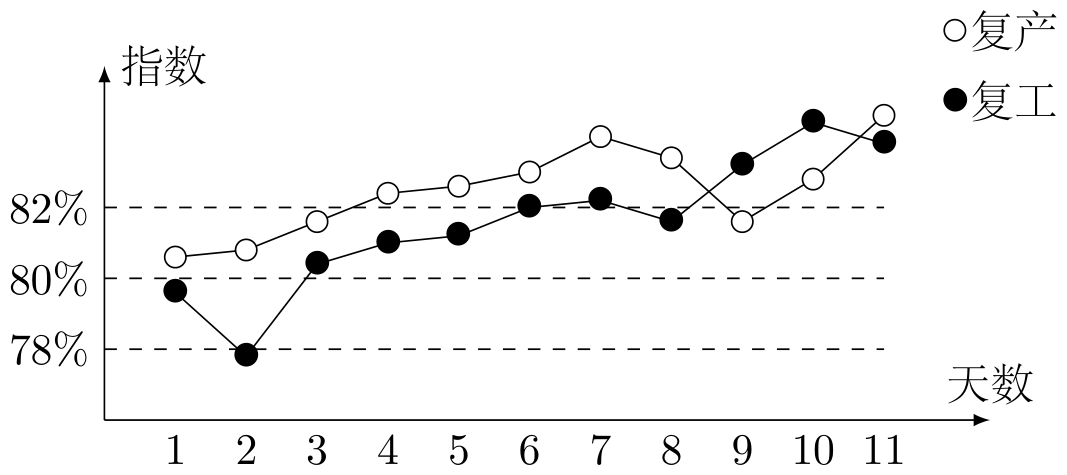
\includegraphics[width=7.6cm]{GaoKao/images/2020/new_gaokao_paper_2/q9_fig1.png}
\par}
        \begin{enumerate}[label=\Alph*.]
            \item 这$11$天复工指数和复产指数均逐日增加
            \item 这$11$天期间，复产指数增量大于复工指数的增量
            \item 第$3$天至第$11$天复工复产指数均超过$80\%$
            \item 第$9$天至第$11$天复产指数增量大于复工指数的增量
        \end{enumerate}
        \item 已知曲线$C:mx^{2}+ny^{2}=1$（\quad）
        \begin{enumerate}[label=\Alph*.]
            \item 若$m>n>0$，则$C$是椭圆，其焦点在$y$轴上
            \item 若$m=n>0$，则$C$是圆，其半径为$\sqrt{n}$
            \item 若$mn<0$，则$C$是双曲线，其渐近线方程为$y=\pm\sqrt{-\dfrac{m}{n}}x$
            \item 若$m=0,n>0$，则$C$是两条直线
        \end{enumerate}
        \item 下图是函数$y=\sin(\omega x+\varphi)$的部分图象，则$\sin(\omega x+\varphi)=$（\quad）
        {\centering
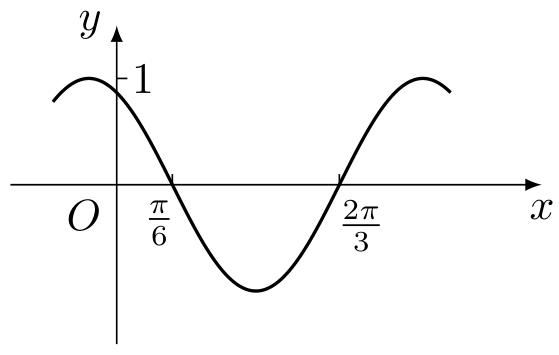
\includegraphics[width=7.9cm]{GaoKao/images/2020/new_gaokao_paper_2/q11_fig1.png}
\par}
        \begin{enumerate}[label=\Alph*.]
            \item $\sin\bigl(x+\frac{\pi}{3}\bigr)$
            \item $\sin\bigl(\frac{\pi}{3}-2x\bigr)$
            \item $\cos\bigl(2x+\frac{\pi}{6}\bigr)$
            \item $\cos\bigl(\frac{5\pi}{6}-2x\bigr)$
        \end{enumerate}
        \item 已知$a>0$，$b>0$，且$a+b=1$，则（\quad）
        \begin{enumerate}[label=\Alph*.]
            \item $a^{2}+b^{2}\geqslant\dfrac{1}{2}$
            \item $2^{a-b}>\dfrac{1}{2}$
            \item $\log_{2}a+\log_{2}b\geqslant -2$
            \item $\sqrt{a}+\sqrt{b}\leqslant\sqrt{2}$
        \end{enumerate}
    \end{enumerate}
    \item[三、填空题]
    \begin{enumerate}[leftmargin=5pt]
      \addtocounter{enumi}{+12}
        \item 棱长为$2$的正方体$ABCD-A_{1}B_{1}C_{1}D_{1}$中，$M,N$分别为棱$BB_{1},AB$的中点，则三棱锥$A-NMD_{1}$的体积为\rule[-0.3ex]{3em}{0.4pt}．
        \item 斜率为$\sqrt{3}$的直线过抛物线$C:y^{2}=4x$的焦点，且与$C$交于$A,B$两点，则$|AB|=\rule[-0.3ex]{3em}{0.4pt}$．
        \item 将数列$\{2n-1\}$与$\{3n-2\}$的公共项从小到大排列得到数列$\{a_{n}\}$，则$\{a_{n}\}$的前$n$项和为\rule[-0.3ex]{6em}{0.4pt}．
        \item 某中学开展劳动实习，学生加工制作零件，零件的截面如图所示．$O$为圆孔及轮廓圆弧$AB$所在圆的圆心，$A$是圆弧$AB$与直线$AG$的切点，$B$是圆弧$AB$与直线$BC$的切点，四边形$DEFG$为矩形，$BC\perp DG$，垂足为$C$，$\tan\angle ODC=\dfrac{3}{5}$，$BH\parallel DG$，$EF=12\text{cm}$，$DE=2\text{cm}$，$A$到直线$DE$和$EF$的距离均为$7\text{cm}$，圆孔半径为$1\text{cm}$，则图中阴影部分的面积为\rule[-0.3ex]{6em}{0.4pt} $\text{cm}^{2}$．
    \end{enumerate}    \item[四、解答题]
    \begin{enumerate}[leftmargin=5pt]
      \addtocounter{enumi}{+16}
        \item 在\ding{172}$ac=\sqrt{3}$，\ding{173}$c\sin A=3$，\ding{174}$c=\sqrt{3}b$这三个条件中任选一个，补充在下面问题中，若问题中的三角形存在，求$c$的值；若问题中的三角形不存在，说明理由．\\
        问题：是否存在$\triangle ABC$，它的内角$A,B,C$的对边分别为$a,b,c$，且$\sin A=\sqrt{3}\sin B$，$C=\dfrac{\pi}{6}$，\rule[-0.3ex]{3em}{0.4pt}？
        \item 已知公比大于$1$的等比数列$\{a_{n}\}$满足$a_{2}+a_{4}=20$，$a_{3}=8$．
        \begin{enumerate}[label=(\arabic*)]
            \item 求$\{a_{n}\}$的通项公式；
            \item 求$a_{1}a_{2}-a_{2}a_{3}+\cdots+(-1)^{n-1}a_{n}a_{n+1}$．
        \end{enumerate}
        \item 为加强环境保护，治理空气污染，环境监测部门对某市空气质量进行调查，随机抽查了$100$天空气中$PM2.5$和$SO_{2}$浓度（单位：$\mu\text{g}/\text{m}^{3}$），得下表：\\
        \begin{tabular}{|c|c|c|c|}
            \hline
            \shortstack{$PM2.5$\\$SO_{2}$} & $[0,50]$ & $(50,150]$ & $(150,475]$ \\
            \hline
            $[0,35]$ & $32$ & $18$ & $4$ \\
            \hline
            $(35,75]$ & $6$ & $8$ & $12$ \\
            \hline
            $(75,115]$ & $3$ & $7$ & $10$ \\
            \hline
        \end{tabular}
        \begin{enumerate}[label=(\arabic*)]
            \item 估计事件``该市一天空气中$PM2.5$浓度不超过$75$，且$SO_{2}$浓度不超过$150$''的概率；
            \item 根据所给数据，完成下面的$2\times 2$列联表：\\
            \begin{tabular}{|c|c|c|}
                \hline
                \shortstack{$PM2.5$\\$SO_{2}$} & $[0,150]$ & $(150,475]$ \\
                \hline
                $[0,75]$ & & \\
                \hline
                $(75,115]$ & & \\
                \hline
            \end{tabular}
            \item 根据$(2)$中的列联表，判断是否有$99\%$的把握认为该市一天空气中$PM2.5$浓度与$SO_{2}$浓度有关？\\
            附：$K^{2}=\dfrac{n(ad-bc)^{2}}{(a+b)(c+d)(a+c)(b+d)}$，
            \begin{tabular}{|c|c|c|c|}
                \hline
                $P(K^{2}\geqslant k)$ & $0.050$ & $0.010$ & $0.001$ \\
                \hline
                $k$ & $3.841$ & $6.635$ & $10.828$ \\
                \hline
            \end{tabular}
        \end{enumerate}        \item 如图，四棱锥$P-ABCD$的底面为正方形，$PD\perp$底面$ABCD$．设平面$PAD$与平面$PBC$的交线为$l$．
        \begin{enumerate}[label=(\arabic*)]
            \item 证明：$l\perp$平面$PDC$；
            \item 已知$PD=AD=1$，$Q$为$l$上的点，$QB=\sqrt{2}$，求$PB$与平面$QCD$所成角的正弦值．
        \end{enumerate}
        \item 已知椭圆$C:\dfrac{x^{2}}{a^{2}}+\dfrac{y^{2}}{b^{2}}=1$（$a>b>0$）过点$M(2,3)$，点$A$为其左顶点，且$AM$的斜率为$\dfrac{1}{2}$．
        \begin{enumerate}[label=(\arabic*)]
            \item 求$C$方程；
            \item 点$N$为椭圆上任意一点，求$\triangle AMN$的面积的最大值．
        \end{enumerate}
        \item 已知函数$f(x)=a\mathrm{e}^{x-1}-\ln x+\ln a$．
        \begin{enumerate}[label=(\arabic*)]
            \item 当$a=\mathrm{e}$时，求曲线$y=f(x)$在点$(1,f(1))$处的切线与两坐标轴围成的三角形的面积；
            \item 若$f(x)\geqslant 1$，求$a$的取值范围．
        \end{enumerate}
    \end{enumerate}
\end{description}
\clearpage

\subsection{2020年北京卷}\label{gk:2020年北京卷}

\begin{description}
    \item[一、选择题]
    \begin{enumerate}[leftmargin=5pt]
        \item 已知集合$A=\{-1,0,1,2\}$，$B=\{x\mid 0<x<3\}$，则$A\cap B=$(\quad)
        
        {\centering\begin{tabular*}{\linewidth}{@{}@{\extracolsep{\fill}}llll@{}}
            \(\text{A. }\{-1,0,1\}\)  & \(\text{B. }\{0,1\}\)  & \(\text{C. }\{-1,1,2\}\)  & \(\text{D. }\{1,2\}\)
        \end{tabular*}\par}

        \item 在复平面内，复数$z$对应的点的坐标是$(1,2)$，则$\i z=$(\quad)
       
        {\centering\begin{tabular*}{\linewidth}{@{}@{\extracolsep{\fill}}llll@{}}
            \(\text{A. }1+2\i\)  & \(\text{B. }-2+\i\)  & \(\text{C. }1-2\i\)  & \(\text{D. }-2-\i\)
        \end{tabular*}\par}

        \item 在$(\sqrt{x}-2)^5$的展开式中，$x^2$的系数为(\quad)
      
        {\centering\begin{tabular*}{\linewidth}{@{}@{\extracolsep{\fill}}llll@{}}
            \(\text{A. }-5\)  & \(\text{B. }5\)  & \(\text{C. }-10\)  & \(\text{D. }10\)
        \end{tabular*}\par}

        \item 某三棱柱的底面为正三角形，其三视图如图所示，该三棱柱的表面积为(\quad)
        {\centering
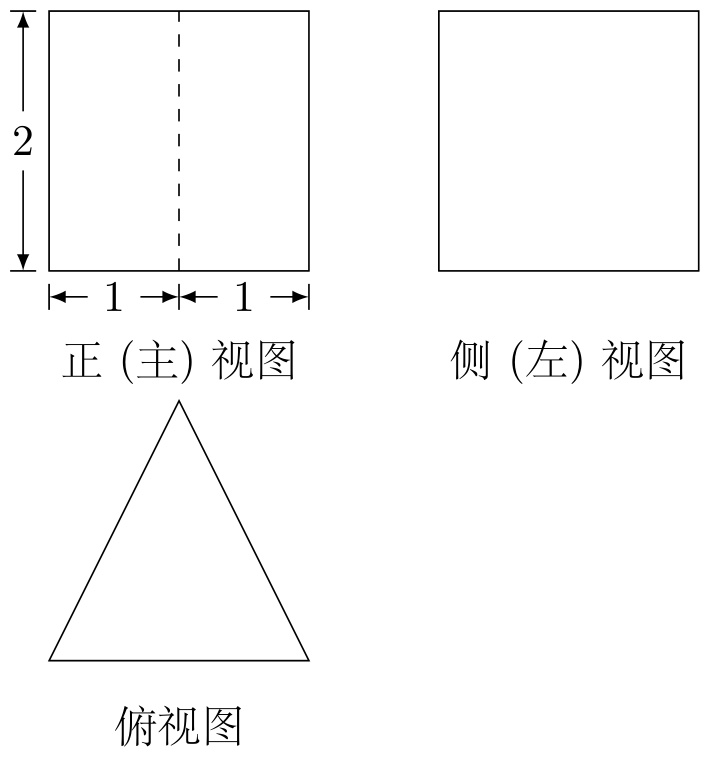
\includegraphics[width=7.0cm]{GaoKao/images/2020/beijing/q4_fig1.png}
\par}
     
        {\centering\begin{tabular*}{\linewidth}{@{}@{\extracolsep{\fill}}llll@{}}
            \(\text{A. }6+\sqrt{3}\)  & \(\text{B. }6+2\sqrt{3}\)  & \(\text{C. }12+\sqrt{3}\)  & \(\text{D. }12+2\sqrt{3}\)
        \end{tabular*}\par}

        \item 已知半径为$1$的圆经过点$(3,4)$，则其圆心到原点的距离的最小值为(\quad)
     
        {\centering\begin{tabular*}{\linewidth}{@{}@{\extracolsep{\fill}}llll@{}}
            \(\text{A. }4\)  & \(\text{B. }5\)  & \(\text{C. }6\)  & \(\text{D. }7\)
        \end{tabular*}\par}

        \item 已知函数$f(x)=2^x-x-1$，则不等式$f(x)>0$的解集是(\quad)
    
        {\centering\begin{tabular*}{\linewidth}{@{}@{\extracolsep{\fill}}llll@{}}
            \(\text{A. }(-1,1)\)  & \(\text{B. }(-\infty,-1)\cup(1,+\infty)\)  & \(\text{C. }(0,1)\)  & \(\text{D. }(-\infty,0)\cup(1,+\infty)\)
        \end{tabular*}\par}

        \item 设抛物线的顶点为$O$，焦点为$F$，准线为$l$．$P$是抛物线上异于$O$的一点，过$P$作$PQ\perp l$于$Q$，则线段$FQ$的垂直平分线(\quad)
    
        {\centering\begin{tabular*}{\linewidth}{@{}@{\extracolsep{\fill}}llll@{}}
            \(\text{A. }\)经过点$O$  & \(\text{B. }\)经过点$P$  & \(\text{C. }\)平行于直线$OP$  & \(\text{D. }\)垂直于直线$OP$
        \end{tabular*}\par}

        \item 在等差数列$\{a_n\}$中，$a_1=-9$，$a_3=-1$．记$T_n=a_1a_2\cdots a_n$($n=1,2,\cdots$)，则数列$\{T_n\}$(\quad)
     
        {\centering\begin{tabular*}{\linewidth}{@{}@{\extracolsep{\fill}}llll@{}}
            \(\text{A. }\)有最大项，有最小项  & \(\text{B. }\)有最大项，无最小项  & \(\text{C. }\)无最大项，有最小项  & \(\text{D. }\)无最大项，无最小项
        \end{tabular*}\par}

        \item 已知$\alpha,\beta\in\mathbb{R}$，则``存在$k\in\mathbb{Z}$使得$\alpha=k\pi+(-1)^k\beta$''是``$\sin\alpha=\sin\beta$''的(\quad)
    
        {\centering\begin{tabular*}{\linewidth}{@{}@{\extracolsep{\fill}}llll@{}}
            \(\text{A. }\)充分而不必要条件  & \(\text{B. }\)必要而不充分条件  & \(\text{C. }\)充分必要条件  & \(\text{D. }\)既不充分也不必要条件
        \end{tabular*}\par}

        \item 2020年3月14日是全球首个国际圆周率日($\pi$~Day)．历史上求圆周率$\pi$的方法有多种，与中国传统数学中的``割圆术''相似，数学家阿尔$\cdot$卡西的方法是：当正整数$n$充分大时，计算单位圆的内接正$6n$边形的周长和外切正$6n$边形(各边均与圆相切的正$6n$边形)的周长，将它们的算术平均数作为$2\pi$的近似值．按照阿尔$\cdot$卡西的方法，$\pi$的近似值的表达式是(\quad)
     
        {\centering\begin{tabular*}{\linewidth}{@{}@{\extracolsep{\fill}}llll@{}}
            \(\text{A. }3n\bigl(\sin\frac{30^\circ}{n}+\tan\frac{30^\circ}{n}\bigr)\)  & \(\text{B. }6n\bigl(\sin\frac{30^\circ}{n}+\tan\frac{30^\circ}{n}\bigr)\)  & \(\text{C. }3n\bigl(\sin\frac{60^\circ}{n}+\tan\frac{60^\circ}{n}\bigr)\)  & \(\text{D. }6n\bigl(\sin\frac{60^\circ}{n}+\tan\frac{60^\circ}{n}\bigr)\)
        \end{tabular*}\par}
    \end{enumerate}

    \item[二、填空题]
    \begin{enumerate}[leftmargin=5pt]
        \addtocounter{enumi}{+10}
        \item 函数$f(x)=\dfrac{1}{x+1}+\ln x$的定义域是\rule[-0.3ex]{3em}{0.4pt}．
        \item 已知双曲线$C:\dfrac{x^2}{6}-\dfrac{y^2}{3}=1$，则$C$的右焦点的坐标为\rule[-0.3ex]{3em}{0.4pt}；$C$的焦点到其渐近线的距离是\rule[-0.3ex]{3em}{0.4pt}．
        \item 已知正方形$ABCD$的边长为$2$，点$P$满足$\overrightarrow{AP}=\dfrac{1}{2}(\overrightarrow{AB}+\overrightarrow{AC})$，则$|\overrightarrow{PD}|=\rule[-0.3ex]{3em}{0.4pt}$；$\overrightarrow{PB}\cdot\overrightarrow{PD}=\rule[-0.3ex]{3em}{0.4pt}$．
        \item 若函数$f(x)=\sin(x+\varphi)+\cos x$的最大值为$2$，则常数$\varphi$的一个取值为\rule[-0.3ex]{3em}{0.4pt}．
        \item 为满足人民对美好生活的向往，环保部门要求相关企业加强污水治理，排放未达标的企业要限期整改．设企业的污水排放量$W$与时间$t$的关系为$W=f(t)$，用$-\dfrac{f(b)-f(a)}{b-a}$的大小评价在$[a,b]$这段时间内企业污水治理能力的强弱，已知整改期内，甲、乙两企业的污水排放量与时间的关系如图所示．
        {\centering
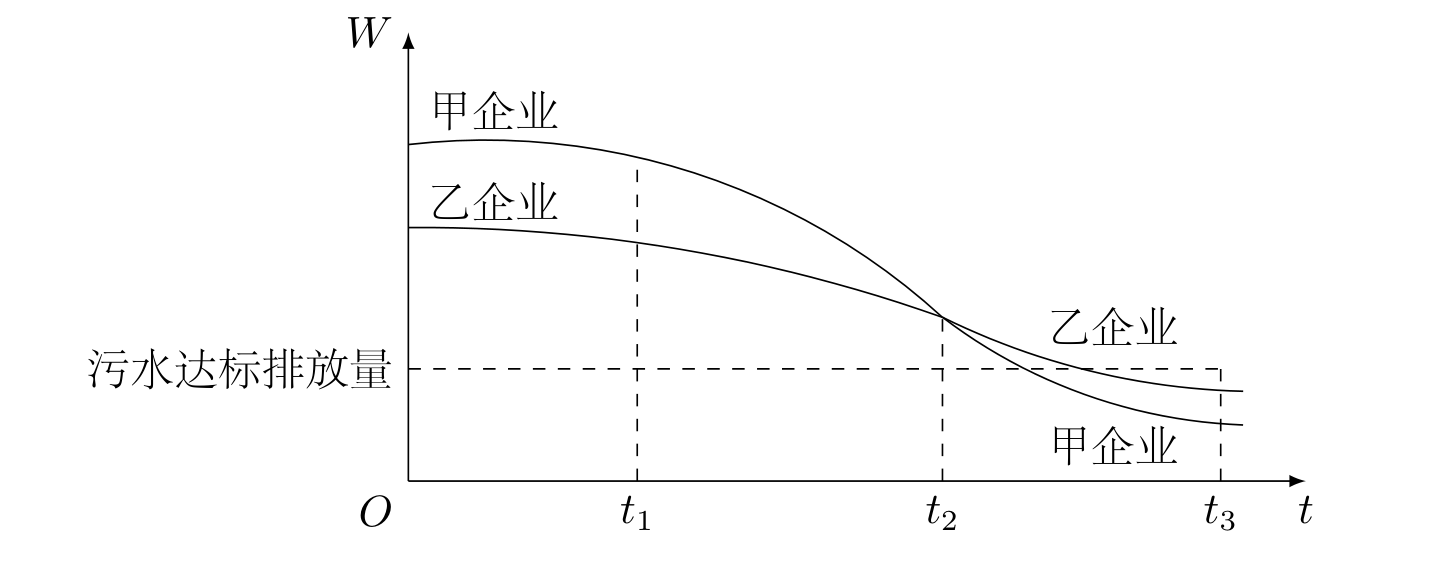
\includegraphics[width=17.0cm]{GaoKao/images/2020/beijing/q15_fig1.png}
\par}
        给出下列四个结论：
        \begin{enumerate}[label=\textcircled{\arabic*}]
            \item 在$[t_1,t_2]$这段时间内，甲企业的污水治理能力比乙企业强；
            \item 在$t_2$时刻，甲企业的污水治理能力比乙企业强；
            \item 在$t_3$时刻，甲、乙两企业的污水排放都已达标；
            \item 甲企业在$[0,t_1]$，$[t_1,t_2]$，$[t_2,t_3]$这三段时间中，在$[0,t_1]$的污水治理能力最强．
        \end{enumerate}
        其中所有正确结论的序号是\rule[-0.3ex]{3em}{0.4pt}．
    \end{enumerate}

    \item[三、解答题]
    \begin{enumerate}[leftmargin=5pt]
        \addtocounter{enumi}{+15}
        \item 如图，在正方体$ABCD-A_1B_1C_1D_1$中，$E$为$BB_1$的中点．
        \begin{enumerate}[label=(\arabic*)]
            \item 求证：$BC_1\parallel$平面$AD_1E$；
            \item 求直线$AA_1$与平面$AD_1E$所成角的正弦值．
        \end{enumerate}
        {\centering
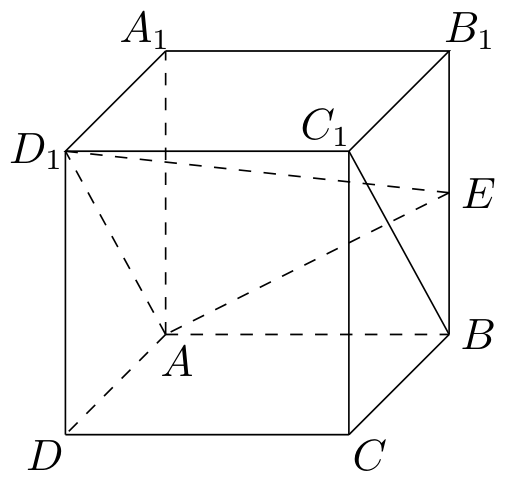
\includegraphics[width=5.0cm]{GaoKao/images/2020/beijing/q16_fig1.png}
\par}

        \item 在$\triangle ABC$中，$a+b=11$，再从条件\ding{172}、条件\ding{173}这两个条件中选择一个作为已知，求：
        \begin{enumerate}[label=(\arabic*)]
            \item $a$的值；
            \item $\sin C$和$\triangle ABC$的面积．
        \end{enumerate}
        条件\ding{172}：$c=7$，$\cos A=-\dfrac{1}{7}$；

        条件\ding{173}：$\cos A=\dfrac{1}{8}$，$\cos B=\dfrac{9}{16}$．

        \item 某校为举办甲、乙两项不同活动，分别设计了相应的活动方案：方案一、方案二．为了解该校学生对活动方案是否支持，对学生进行简单随机抽样，获得数据如下表：
        \begin{center}
\begin{tabular}{c|cc|cc}
\hline
& \multicolumn{2}{c|}{男生} & \multicolumn{2}{c}{女生} \\
\hline
& 支持 & 不支持 & 支持 & 不支持 \\
\hline
方案一 & $200\text{ 人}$ & $400\text{ 人}$ & $300\text{ 人}$ & $100\text{ 人}$ \\
方案二 & $350\text{ 人}$ & $250\text{ 人}$ & $150\text{ 人}$ & $250\text{ 人}$ \\
\hline
\end{tabular}
\end{center}
        假设所有学生对活动方案是否支持相互独立．
        \begin{enumerate}[label=(\arabic*)]
            \item 分别估计该校男生支持方案一的概率、该校女生支持方案一的概率；
            \item 从该校全体男生中随机抽取$2$人，全体女生中随机抽取$1$人，估计这$3$人中恰有$2$人支持方案一的概率；
            \item 将该校学生支持方案的概率估计值记为$p_0$，假设该校一年级有$500$名男生和$300$名女生，除一年级外其他年级学生支持方案二的概率估计值记为$p_1$，试比较$p_0$与$p_1$的大小．(结论不要求证明)
        \end{enumerate}

        \item 已知函数$f(x)=12-x^2$．
        \begin{enumerate}[label=(\arabic*)]
            \item 求曲线$y=f(x)$的斜率等于$-2$的切线方程；
            \item 设曲线$y=f(x)$在点$(t,f(t))$处的切线与坐标轴围成的三角形的面积为$S(t)$，求$S(t)$的最小值．
        \end{enumerate}

        \item 已知椭圆$C:\dfrac{x^2}{a^2}+\dfrac{y^2}{b^2}=1$过点$A(-2,-1)$，且$a=2b$．
        \begin{enumerate}[label=(\arabic*)]
            \item 求椭圆$C$的方程；
            \item 过点$B(-4,0)$的直线$l$交椭圆$C$于点$M,N$，直线$MA,NA$分别交直线$x=-4$于点$P,Q$．求$\dfrac{|PB|}{|BQ|}$的值．
        \end{enumerate}

        \item 已知$\{a_n\}$是无穷数列．给出两个性质：
        \begin{enumerate}[label=\textcircled{\arabic*}]
            \item 对于$\{a_n\}$中任意两项$a_i,a_j(i>j)$，在$\{a_n\}$中都存在一项$a_m$，使得$\dfrac{a_i^2}{a_j}=a_m$；
            \item 对于$\{a_n\}$中任意项$a_n(n\geqslant 3)$，在$\{a_n\}$中都存在两项$a_k,a_l(k>l)$，使得$a_n=\dfrac{a_k^2}{a_l}$．
        \end{enumerate}
        \begin{enumerate}[label=(\arabic*)]
            \item 若$a_n=n(n=1,2,\cdots)$，判断数列$\{a_n\}$是否满足性质\ding{172}，说明理由；
            \item 若$a_n=2^{n-1}(n=1,2,\cdots)$，判断数列$\{a_n\}$是否同时满足性质\ding{172}和性质\ding{173}，说明理由；
            \item 若$\{a_n\}$是递增数列，且同时满足性质\ding{172}和性质\ding{173}，证明：$\{a_n\}$为等比数列．
        \end{enumerate}
    \end{enumerate}
\end{description}
\clearpage


\subsection{2020年江苏卷}\label{gk:2020年江苏卷}

\begin{description}
    \item[一、填空题]
    \begin{enumerate}[leftmargin=5pt]
        \item 已知集合$A=\{-1,0,1,2\}$，$B=\{0,2,3\}$，则$A\cap B=\rule[-0.3ex]{3em}{0.4pt}$．
        \item 已知$\i$是虚数单位，则复数$z=(1+\i)(2-\i)$的实部是\rule[-0.3ex]{3em}{0.4pt}．
        \item 已知一组数据$4,2a,3-a,5,6$的平均数为$4$，则$a$的值是\rule[-0.3ex]{3em}{0.4pt}．
        \item 将一颗质地均匀的正方体骰子先后抛掷$2$次，观察向上的点数，则点数和为$5$的概率是\rule[-0.3ex]{3em}{0.4pt}．
        \item 如图是一个算法流程图．若输出$y$的值为$-2$，则输入$x$的值是\rule[-0.3ex]{3em}{0.4pt}．
        {\centering
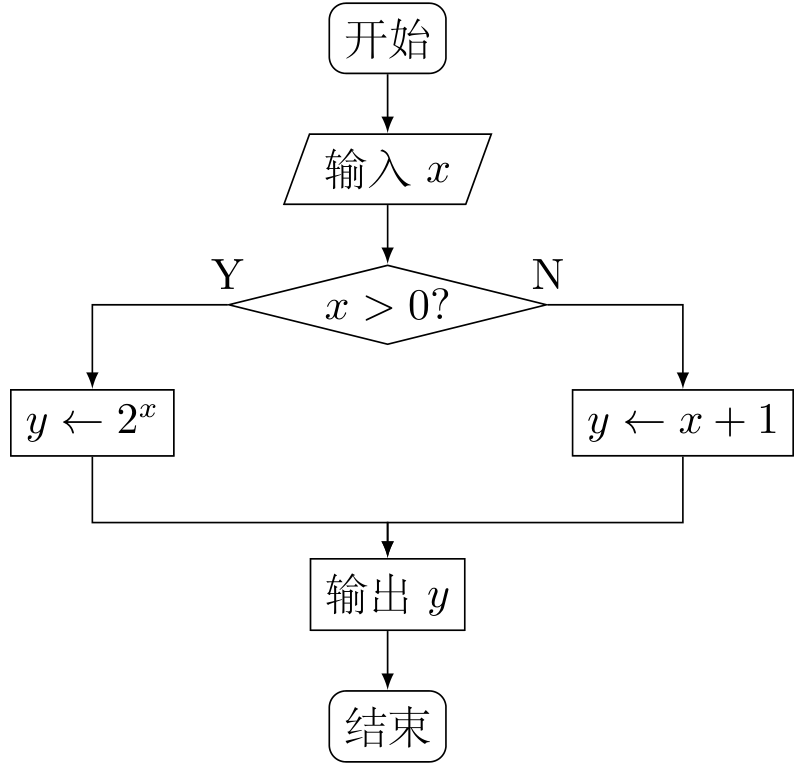
\includegraphics[width=5.1cm]{GaoKao/images/2020/jiangsu/q5_fig1.png}
\par}
        \item 在平面直角坐标系$xOy$中，若双曲线$\dfrac{x^2}{a^2}-\dfrac{y^2}{5}=1(a>0)$的一条渐近线方程为$y=\dfrac{\sqrt{5}}{2}x$，则该双曲线的离心率是\rule[-0.3ex]{3em}{0.4pt}．
        \item 已知$y=f(x)$是奇函数，当$x\geqslant 0$时，$f(x)=x^{\frac{2}{3}}$，则$f(-8)$的值是\rule[-0.3ex]{3em}{0.4pt}．
        \item 已知$\sin^2\bigl(\frac{\pi}{4}+\alpha\bigr)=\frac{2}{3}$，则$\sin2\alpha$的值是\rule[-0.3ex]{3em}{0.4pt}．
        \item 如图，六角螺帽毛坯是由一个正六棱柱挖去一个圆柱所构成的．已知螺帽的底面正六边形边长为$2\,\text{cm}$，高为$2\,\text{cm}$，内孔半径为$0.5\,\text{cm}$，则此六角螺帽毛坯的体积是\rule[-0.3ex]{3em}{0.4pt}$\,\text{cm}^3$．
        \item 将函数$y=3\sin\bigl(2x+\frac{\pi}{4}\bigr)$的图象向右平移$\frac{\pi}{6}$个单位长度，则平移后的图象中与$y$轴最近的对称轴的方程是\rule[-0.3ex]{3em}{0.4pt}．
        \item 设$\{a_n\}$是公差为$d$的等差数列，$\{b_n\}$是公比为$q$的等比数列．已知数列$\{a_n+b_n\}$的前$n$项和$S_n=n^2-n+2^n-1\,(n\in\mathbb{N}^*)$，则$d+q$的值是\rule[-0.3ex]{3em}{0.4pt}．
        \item 已知$5x^2y^2+y^4=1\,(x,y\in\mathbb{R})$，则$x^2+y^2$的最小值是\rule[-0.3ex]{3em}{0.4pt}．
        \item 在$\triangle ABC$中，$AB=4$，$AC=3$，$\angle BAC=90^\circ$，$D$在边$BC$上，延长$AD$到$P$，使得$AP=9$，若$\overrightarrow{PA}=m\overrightarrow{PB}+\bigl(\frac{3}{2}-m\bigr)\overrightarrow{PC}$($m$为常数)，则$CD$的长度是\rule[-0.3ex]{3em}{0.4pt}．
        \item 在平面直角坐标系$xOy$中，已知$P\bigl(\frac{\sqrt{3}}{2},0\bigr)$，$A,B$是圆$C:x^2+\bigl(y-\frac{1}{2}\bigr)^2=36$上的两个动点，满足$PA=PB$，则$\triangle PAB$面积的最大值是\rule[-0.3ex]{3em}{0.4pt}．
    \end{enumerate}

    \item[二、解答题]
    \begin{enumerate}[leftmargin=5pt]
        \addtocounter{enumi}{+14}
        \item 在三棱柱$ABC-A_1B_1C_1$中，$AB\perp AC$，$B_1C\perp$平面$ABC$，$E,F$分别是$AC,B_1C$的中点．
        \begin{enumerate}[label=(\arabic*)]
            \item 求证：$EF\parallel$平面$AB_1C_1$；
            \item 求证：平面$AB_1C\perp$平面$ABB_1$．
        \end{enumerate}
        {\centering
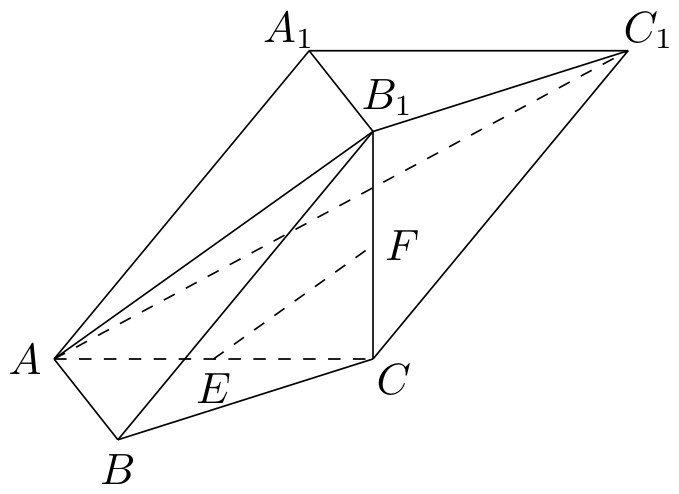
\includegraphics[width=7.0cm]{GaoKao/images/2020/jiangsu/q15_fig1.png}
\par}

        \item 在$\triangle ABC$中，角$A,B,C$的对边分别为$a,b,c$，已知$a=3$，$c=\sqrt{2}$，$B=45^\circ$．
        \begin{enumerate}[label=(\arabic*)]
            \item 求$\sin C$的值；
            \item 在边$BC$上取一点$D$，使得$\cos\angle ADC=-\dfrac{4}{5}$，求$\tan\angle DAC$的值．
        \end{enumerate}

        \item 某地准备在山谷中建一座桥梁，桥址位置的竖直截面图如图所示：谷底$O$在水平线$MN$上．桥$AB$与$MN$平行，$OO'$为铅垂线($O'$在$AB$上)．经测量，左侧曲线$AO$上任一点$D$到$MN$的距离$h_1$(米)与$D$到$OO'$的距离$a$(米)之间满足关系式$h_1=\frac{1}{40}a^2$；右侧曲线$BO$上任一点$F$到$MN$的距离$h_2$(米)与$F$到$OO'$的距离$b$(米)之间满足关系式$h_2=-\frac{1}{800}b^3+6b$．已知点$B$到$OO'$的距离为$40$米．
        \begin{enumerate}[label=(\arabic*)]
            \item 求桥$AB$的长度；
            \item 计划在谷底两侧建造平行于$OO'$的桥墩$CD$和$EF$，且$CE$为$90$米，其中$C,E$在$AB$上(不包括端点)．桥墩$EF$每米造价$k$(万元)、桥墩$CD$每米造价$\frac{3}{2}k$(万元)($k>0$)．问$O'E$为多少米时，桥墩$CD$与$EF$的总造价最低？
        \end{enumerate}
        {\centering
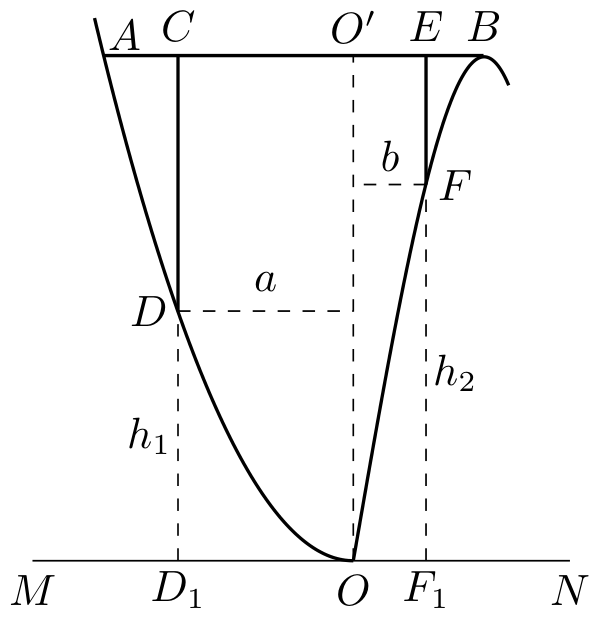
\includegraphics[width=6.2cm]{GaoKao/images/2020/jiangsu/q17_fig1.png}
\par}

        \item 在平面直角坐标系$xOy$中，已知椭圆$E:\dfrac{x^2}{4}+\dfrac{y^2}{3}=1$的左、右焦点分别为$F_1,F_2$，点$A$在椭圆$E$上且在第一象限内，$AF_2\perp F_1F_2$，直线$AF_1$与椭圆$E$相交于另一点$B$．
        \begin{enumerate}[label=(\arabic*)]
            \item 求$\triangle AF_1F_2$的周长；
            \item 在$x$轴上任取一点$P$，直线$AP$与椭圆$E$的右准线相交于点$Q$，求$\overrightarrow{OP}\cdot\overrightarrow{QP}$的最小值；
            \item 设点$M$在椭圆$E$上，记$\triangle OAB$与$\triangle MAB$的面积分别为$S_1,S_2$，若$S_2=3S_1$，求点$M$的坐标．
        \end{enumerate}

        \item 已知关于$x$的函数$y=f(x)$，$y=g(x)$与$h(x)=kx+b$($k,b\in\mathbb{R}$)在区间$D$上恒有$f(x)\geqslant h(x)\geqslant g(x)$．
        \begin{enumerate}[label=(\arabic*)]
            \item 若$f(x)=x^2+2x$，$g(x)=-x^2+2x$，$D=(-\infty,+\infty)$，求$h(x)$的表达式；
            \item 若$f(x)=x^2-x+1$，$g(x)=k\ln x$，$h(x)=kx-k$，$D=(0,+\infty)$，求$k$的取值范围；
            \item 若$f(x)=x^4-2x^2$，$g(x)=4x^2-8$，$h(x)=4(t^3-t)x-3t^4+2t^2$($0<|t|\leqslant\sqrt{2}$)，$D=[m,n]\subseteq[-\sqrt{2},\sqrt{2}]$，求证：$n-m\leqslant\sqrt{7}$．
        \end{enumerate}

        \item 已知数列$\{a_n\}(n\in\mathbb{N}^*)$的首项$a_1=1$，前$n$项和为$S_n$．设$\lambda$与$k$是常数，若对一切正整数$n$，均有$S_{n+1}^{\frac{1}{k}}-S_n^{\frac{1}{k}}=\lambda a_{n+1}^{\frac{1}{k}}$成立，则称此数列为``$\lambda\sim k$''数列．
        \begin{enumerate}[label=(\arabic*)]
            \item 若等差数列$\{a_n\}$是``$\lambda\sim 1$''数列，求$\lambda$的值；
            \item 若数列$\{a_n\}$是``$\frac{\sqrt{3}}{3}\sim 2$''数列，且$a_n>0$，求数列$\{a_n\}$的通项公式；
            \item 对于给定的$\lambda$，是否存在三个不同的数列$\{a_n\}$为``$\lambda\sim 3$''数列，且$a_n\geqslant 0$？若存在，求$\lambda$的取值范围；若不存在，说明理由．
        \end{enumerate}
    \end{enumerate}

    \item[三、选做题（三选二）]
    \begin{enumerate}[leftmargin=5pt]
        \addtocounter{enumi}{+20}
        \item \textbf{【A．矩阵与变换】}平面上点$A(2,-1)$在矩阵$M=\begin{bmatrix}a&1\\-1&b\end{bmatrix}$对应的变换作用下得到点$B(3,-4)$．
        \begin{enumerate}[label=(\arabic*)]
            \item 求实数$a,b$的值；
            \item 求矩阵$M$的逆矩阵$M^{-1}$．
        \end{enumerate}

        \textbf{【B．坐标系与参数方程】}在极坐标系中，已知点$A(\rho_1,\frac{\pi}{3})$在直线$l:\rho\cos\theta=2$上，点$B(\rho_2,\frac{\pi}{6})$在圆$C:\rho=4\sin\theta$上，其中$\rho\geqslant 0$，$0\leqslant\theta<2\pi$．
        \begin{enumerate}[label=(\arabic*)]
            \item 求$\rho_1,\rho_2$的值；
            \item 求出直线$l$与圆$C$的公共点的极坐标．
        \end{enumerate}

        \textbf{【C．不等式选讲】}设$x\in\mathbb{R}$，解不等式$2|x+1|+|x|\leqslant 4$．
    \end{enumerate}

    \item[四、附加题]
    \begin{enumerate}[leftmargin=5pt]
        \addtocounter{enumi}{+21}
        \item 在三棱锥$A-BCD$中，已知$CB=CD=\sqrt{5}$，$BD=2$，$O$为$BD$的中点，$AO\perp$平面$BCD$，$AO=2$，$E$为$AC$的中点．
        \begin{enumerate}[label=(\arabic*)]
            \item 求直线$AB$与$DE$所成角的余弦值；
            \item 若点$F$在$BC$上，满足$BF=\frac{1}{4}BC$，设二面角$F-DE-C$的大小为$\theta$，求$\sin\theta$的值．
        \end{enumerate}
        {\centering
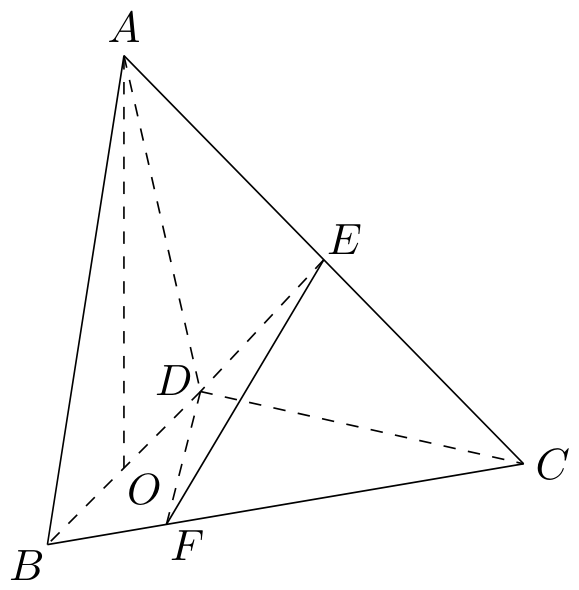
\includegraphics[width=10.0cm]{GaoKao/images/2020/jiangsu/q24_fig1.png}
\par}

        \item 甲口袋中装有$2$个黑球和$1$个白球，乙口袋中装有$3$个白球．现从甲、乙两口袋中各任取一个球交换放入另一口袋，重复$n$次这样的操作，记甲口袋中黑球个数为$X_n$，恰有$2$个黑球的概率为$p_n$，恰有$1$个黑球的概率为$q_n$．
        \begin{enumerate}[label=(\arabic*)]
            \item 求$p_1,q_1$和$p_2,q_2$；
            \item 求$2p_n+q_n$与$2p_{n-1}+q_{n-1}$的递推关系式和$X_n$的数学期望$E(X_n)$(用$n$表示)．
        \end{enumerate}
    \end{enumerate}
\end{description}
\clearpage

\subsection{2020年上海卷}\label{gk:2020年上海卷}

\begin{description}
    \item[一、填空题]
    \begin{enumerate}[leftmargin=5pt]
        \item 若集合$A=\{1,2,4\}$，$B=\{2,4,5\}$，则$A\cap B=\rule[-0.3ex]{3em}{0.4pt}$．
        \item 计算：$\lim\limits_{n\to\infty}\dfrac{n+1}{3n-1}=\rule[-0.3ex]{3em}{0.4pt}$．
        \item 若复数$z=1-2\i$（其中$\i$为虚数单位），则$|z|=\rule[-0.3ex]{3em}{0.4pt}$．
        \item 函数$f(x)=x^{3}$的反函数为\rule[-0.3ex]{6em}{0.4pt}．
        \item 若实数$x,y$满足$\begin{cases}x+y-2\geqslant 0,\\ x+2y-3\leqslant 0,\\ y\geqslant 0,\end{cases}$则$z=y-2x$的最大值为\rule[-0.3ex]{3em}{0.4pt}．
        \item 设$a,b,c,d\in\mathbb{R}$，若行列式$\begin{vmatrix}1&a&b\\2&c&d\\3&0&0\end{vmatrix}=6$，则行列式$\begin{vmatrix}a&b\\c&d\end{vmatrix}=\rule[-0.3ex]{3em}{0.4pt}$．
        \item 设$a,b\in\mathbb{R}$，若$1,2,a,b$这四个数的中位数为$3$，平均数为$4$，则$ab=\rule[-0.3ex]{3em}{0.4pt}$．
        \item 已知公差不为$0$的等差数列$\{a_{n}\}$，其前$n$项和为$S_{n}$，若$a_{1}+a_{10}=a_{9}$，则$\dfrac{S_{9}}{a_{10}}=\rule[-0.3ex]{3em}{0.4pt}$．
        \item 从$5$人中选出$4$人去值班，每人值班一天，若第一天安排$1$人，第二天安排$1$人，第三天安排$2$人，则不同安排方法的种数为\rule[-0.3ex]{3em}{0.4pt}（结果用数值表示）．
        \item 已知椭圆$\Gamma:\dfrac{x^{2}}{4}+\dfrac{y^{2}}{3}=1$的右焦点为$F$，点$P$位于第二象限且在$\Gamma$上，联结$PF$并延长交$\Gamma$于点$Q(x_{Q},y_{Q})$，点$Q'(x_{Q'},y_{Q'})$也在$\Gamma$上，且$y_{Q}+y_{Q'}=0$．若$\overrightarrow{QF}=\overrightarrow{FP}$，则直线$PQ$的方程为\rule[-0.3ex]{10em}{0.4pt}．
        \item 设$a\in\mathbb{R}$，若存在定义域为$\mathbb{R}$的函数$f(x)$既满足``对任意$x_{0}\in\mathbb{R}$，$f(x_{0})$的值为$x_{0}^{2}$或$x_{0}$''又满足``关于$x$的方程$f(x)=a$无实数解''，则$a$取值范围是\rule[-0.3ex]{6em}{0.4pt}．
        \item 已知$\bm{a}_{1},\bm{a}_{2},\bm{b}_{1},\bm{b}_{2},\cdots,\bm{b}_{k}$是平面内两两互不相等的向量，若$|\bm{a}_{1}-\bm{a}_{2}|=1$，且$|\bm{a}_{i}-\bm{b}_{j}|\in\{1,2\}$（其中$i=1,2$，$j=1,2,\cdots,k$），则$k$最大值为\rule[-0.3ex]{3em}{0.4pt}．
    \end{enumerate}    \item[二、选择题]
    \begin{enumerate}[leftmargin=5pt]
      \addtocounter{enumi}{+12}
        \item 若$a,b\in\mathbb{R}$，则下列不等式中恒成立的是（\quad）
        {\centering\begin{tabular*}{\linewidth}{@{}@{\extracolsep{\fill}}llll@{}}
            $\text{A. }a^{2}+b^{2}\geqslant 2ab$  & $\text{B. }a^{2}+b^{2}\geqslant -2ab$  & $\text{C. }a+b\geqslant 2\sqrt{|ab|}$  & $\text{D. }a+b\geqslant -2\sqrt{|ab|}$
        \end{tabular*}\par}
        \item 直线$3x+4y+1=0$的一个参数方程可以为（\quad）
        {\centering\begin{tabular*}{\linewidth}{@{}@{\extracolsep{\fill}}llll@{}}
            $\text{A. }\begin{cases}x=1+3t,\\y=-1+4t\end{cases}(t\text{为参数})$  & $\text{B. }\begin{cases}x=1-3t,\\y=-1+4t\end{cases}(t\text{为参数})$  & $\text{C. }\begin{cases}x=1-4t,\\y=-1-3t\end{cases}(t\text{为参数})$  & $\text{D. }\begin{cases}x=1+4t,\\y=-1-3t\end{cases}(t\text{为参数})$
        \end{tabular*}\par}
        \item 在如图所示的棱长为$10$的正方体$ABCD-A_{1}B_{1}C_{1}D_{1}$中，一条平行于$A_{1}C$的直线与正方体的表面交于$P,Q$两点，其中$P$在侧面$ADD_{1}A_{1}$上，且到$A_{1}D_{1}$的距离为$3$，到$AA_{1}$的距离为$2$，则点$Q$所在的面是（\quad）
        {\centering\begin{tabular*}{\linewidth}{@{}@{\extracolsep{\fill}}llll@{}}
            $\text{A. }ABCD$  & $\text{B. }ABB_{1}A_{1}$  & $\text{C. }BCC_{1}B_{1}$  & $\text{D. }CDD_{1}C_{1}$
        \end{tabular*}\par}
        \item 对于定义在$\mathbb{R}$上的函数$y=f(x)$，考察以下性质：\\
        $p$：存在非零实数$a$，使得$f(x+a)<f(x)+f(a)$对任意的$x\in\mathbb{R}$恒成立；\\
        $q_{1}$：$y=f(x)$单调递减，且$f(x)$恒大于$0$；\\
        $q_{2}$：$y=f(x)$单调递增，且存在$x_{0}<0$，使得$f(x_{0})=0$．\\
        关于上述性质，以下判断正确的是（\quad）
        {\centering\begin{tabular*}{\linewidth}{@{}@{\extracolsep{\fill}}llll@{}}
            $\text{A. }q_{1},q_{2}\text{都是}p\text{的充分条件}$  & $\text{B. }q_{1},q_{2}\text{中仅}q_{1}\text{是}p\text{的充分条件}$  & $\text{C. }q_{1},q_{2}\text{中仅}q_{2}\text{是}p\text{的充分条件}$  & $\text{D. }q_{1},q_{2}\text{都不是}p\text{的充分条件}$
        \end{tabular*}\par}
    \end{enumerate}
    \item[三、解答题]
    \begin{enumerate}[leftmargin=5pt]
      \addtocounter{enumi}{+16}
        \item 如图所示，边长为$1$的正方形$ABCD$绕$BC$边旋转后形成一个圆柱．
        \begin{enumerate}[label=(\arabic*)]
            \item 求该圆柱表面积$S$；
            \item 正方形$ABCD$绕$BC$逆时针旋转$\dfrac{\pi}{2}$到$A_{1}BCD_{1}$，求$AD_{1}$与平面$ABCD$所成角的大小（结果用反三角函数值表示）．
        \end{enumerate}
        \item 已知函数$f(x)=\sin\omega x$（$\omega>0$）．
        \begin{enumerate}[label=(\arabic*)]
            \item 若函数$y=f(x)$的周期为$4\pi$，求$\omega$及此时$f(x)=\dfrac{1}{2}$的解集；
            \item 若$\omega=1$，设$g(x)=f^{2}(x)+\sqrt{3}f(-x)\cdot f\Bigl(\dfrac{\pi}{2}-x\Bigr)$，$x\in\Bigl[0,\dfrac{\pi}{4}\Bigr]$，求函数$y=g(x)$值域．
        \end{enumerate}        \item 在研究某市交通情况时，道路密度是指该路段上一定时间内通过的车辆数量除以时间，车辆密度是指该路段一定时间内通过的车辆数除以该路段的长度．现定义交通流量为$v=\dfrac{q}{x}$，其中$x$为道路密度，$q$为车辆密度．据调查某路段的交通流量有如下规律：$$v=\begin{cases}100-135\cdot\Bigl(\dfrac{1}{3}\Bigr)^{\frac{80}{x}},&0<x<40,\\[6pt]-k(x-40)+85,&40\leqslant x\leqslant 60,\end{cases}$$（其中$k>0$）．
        \begin{enumerate}[label=(\arabic*)]
            \item 当交通流量大于$95$时，求道路密度$x$的取值范围；
            \item 若道路密度$x=80$时，测得交通流量$v=50$，求车辆密度$q$的最大值．
        \end{enumerate}
        \item 设$b>0$．如图所示，在平面直角坐标系$xOy$中，$A(x_{A},y_{A})$是双曲线$C_{1}:\dfrac{x^{2}}{4}-\dfrac{y^{2}}{b^{2}}=1$和圆$C_{2}:x^{2}+y^{2}=4+b^{2}$在第一象限内的交点，曲线$\Gamma$由$C_{1}$中满足$|x|\geqslant x_{A}$的部分和$C_{2}$中满足$|x|\leqslant x_{A}$的部分构成．
        \begin{enumerate}[label=(\arabic*)]
            \item 若$x_{A}=\sqrt{6}$，求$b$的值；
            \item 若$b=\sqrt{5}$，$F_{1},F_{2}$分别为$\Gamma$与$x$轴的左、右两个交点，第一象限内的点$P$也在$\Gamma$上，且$|PF_{1}|=8$，求$\angle F_{1}PF_{2}$的大小；
            \item 过点$S\Bigl(0,\dfrac{b^{2}}{2}+2\Bigr)$作斜率为$-\dfrac{b}{2}$的直线$l$．若$l$与$\Gamma$恰有两个不同的公共点，记为$M,N$，用$b$表示$\overrightarrow{OM}\cdot\overrightarrow{ON}$，并求当$b$变化时，$\overrightarrow{OM}\cdot\overrightarrow{ON}$的取值范围．
        \end{enumerate}
        \item 对于至少有三项的有穷实数数列$\{a_{n}\}$，若$|a_{2}-a_{1}|\leqslant|a_{3}-a_{1}|\leqslant\cdots\leqslant|a_{m}-a_{1}|$（其中$m$为$\{a_{n}\}$的项数），则称具有性质$P$．
        \begin{enumerate}[label=(\arabic*)]
            \item 分别判断数列$3,2,5,1$与数列$4,3,2,5,1$是否具有性质$P$，并说明理由；
            \item 已知首项为$1$，公比为$q$，项数为$10$的等比数列$\{a_{n}\}$具有性质$P$，求$q$的取值范围；
            \item 给定正整数$m\geqslant 3$．设数列$\{a_{n}\}$是$1,2,\cdots,m$的一个排列，项数为$m-1$的数列$\{b_{n}\}$满足$b_{k}=a_{k}-1$（$k=1,2,\cdots,m-1$），且$\{a_{n}\}$与$\{b_{n}\}$都具有性质$P$，求所有满足条件的数列$\{a_{n}\}$．
        \end{enumerate}
    \end{enumerate}
\end{description}
\clearpage


\subsection{2020年天津卷}\label{gk:2020年天津卷}

\begin{description}
    \item[一、选择题]
    \begin{enumerate}[leftmargin=5pt]
        \item 设全集$U=\{-3,-2,-1,0,1,2,3\}$，集合$A=\{-1,0,1,2\}$，$B=\{-3,0,2,3\}$，则$A\cap(\complement_{U}B)=$（\quad）
        {\centering\begin{tabular*}{\linewidth}{@{}@{\extracolsep{\fill}}llll@{}}
            $\text{A. }\{-3,3\}$  & $\text{B. }\{0,2\}$  & $\text{C. }\{-1,1\}$  & $\text{D. }\{-3,-2,-1,1,3\}$
        \end{tabular*}\par}
        \item 设$a\in\mathbb{R}$，则``$a>1$''是``$a^{2}>a$''的（\quad）
        {\centering\begin{tabular*}{\linewidth}{@{}@{\extracolsep{\fill}}llll@{}}
            $\text{A. }$充分不必要条件  & $\text{B. }$必要不充分条件  & $\text{C. }$充要条件  & $\text{D. }$既不充分也不必要条件
        \end{tabular*}\par}        \item 函数$y=\dfrac{4x}{x^{2}+1}$的图象大致为（\quad）
        
        {\centering\begin{tabular*}{\linewidth}{@{}@{\extracolsep{\fill}}cccc@{}}
            \(\text{A. }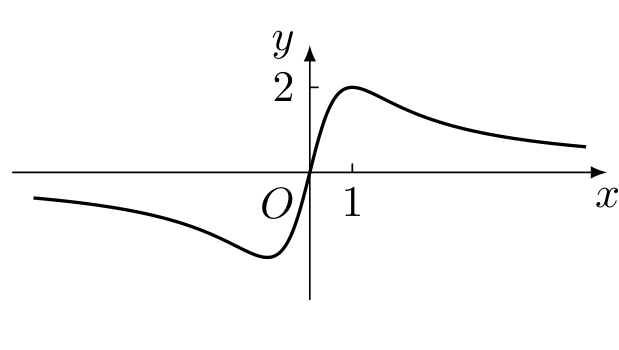
\includegraphics[width=0.15\paperwidth]{GaoKao/images/2020/tianjin/q3_fig1.png}\)  &  \(\text{B. }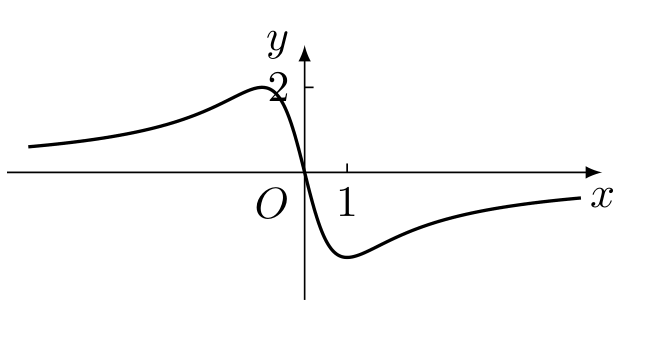
\includegraphics[width=0.15\paperwidth]{GaoKao/images/2020/tianjin/q3_fig2.png}\)  &  \(\text{C. }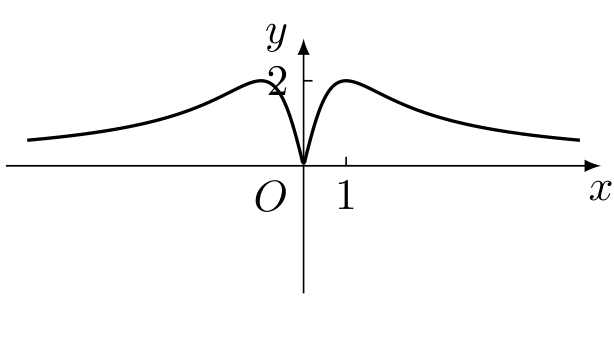
\includegraphics[width=0.15\paperwidth]{GaoKao/images/2020/tianjin/q3_fig3.png}\)  &  \(\text{D. }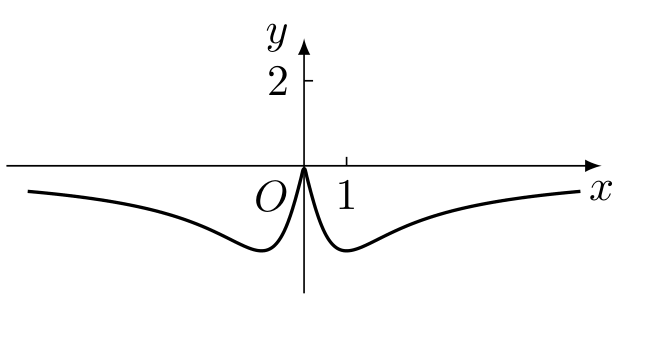
\includegraphics[width=0.15\paperwidth]{GaoKao/images/2020/tianjin/q3_fig4.png}\)
        \end{tabular*}\par}
        \item 从一批零件中抽取$80$个，测量其直径（单位：mm），将所得数据分为$9$组：$[5.31,5.33)$，$[5.33,5.35)$，$\cdots$，$[5.45,5.47)$，$[5.47,5.49]$，并整理得到如下频率分布直方图，则在被抽取的零件中，直径落在区间$[5.43,5.47)$内的个数为（\quad）
        {\centering
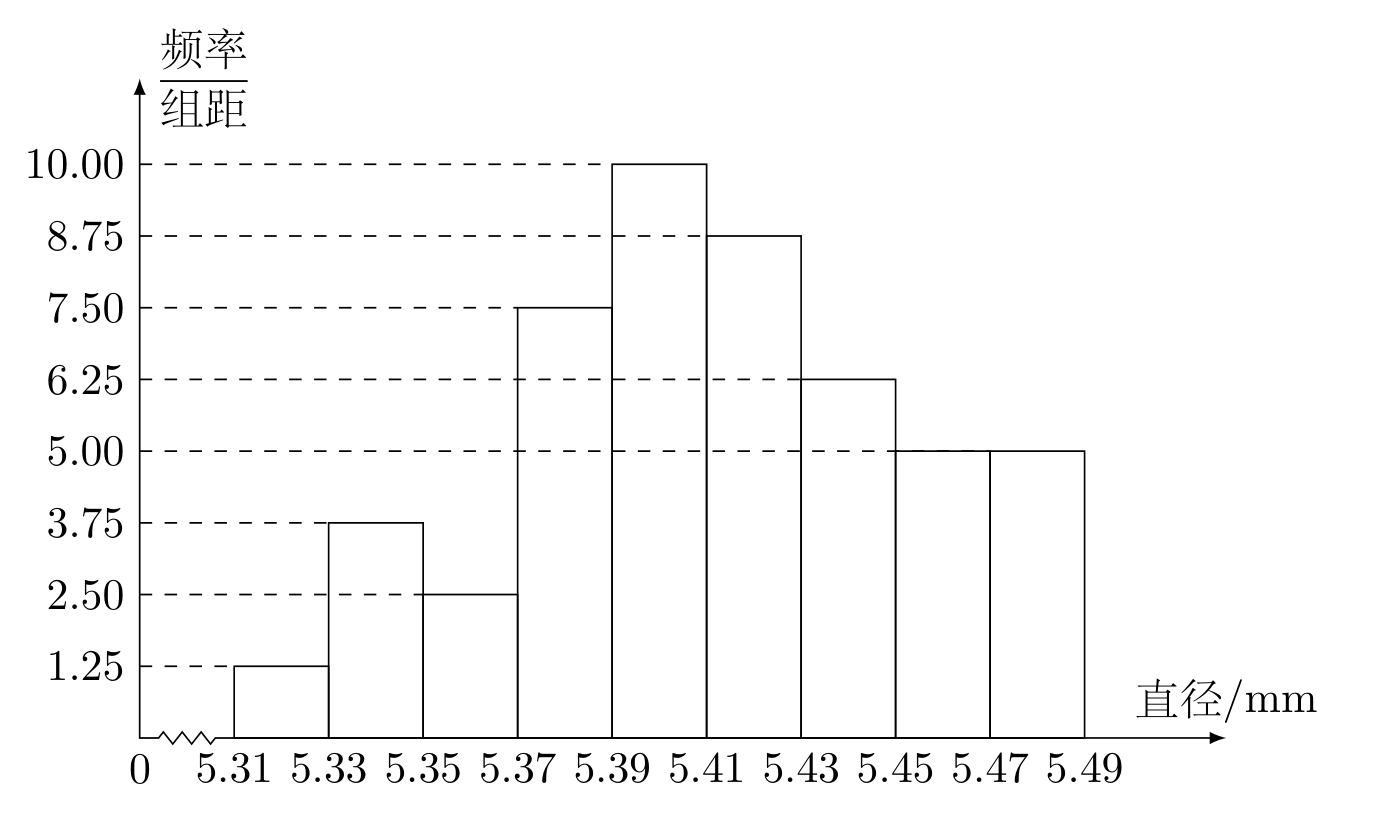
\includegraphics[width=0.65\linewidth]{GaoKao/images/2020/tianjin/q4_fig1.png}
\par}
        {\centering\begin{tabular*}{\linewidth}{@{}@{\extracolsep{\fill}}llll@{}}
            $\text{A. }10$  & $\text{B. }18$  & $\text{C. }20$  & $\text{D. }36$
        \end{tabular*}\par}
        \item 若棱长为$2\sqrt{3}$的正方体的顶点都在同一球面上，则该球的表面积为（\quad）
        {\centering\begin{tabular*}{\linewidth}{@{}@{\extracolsep{\fill}}llll@{}}
            $\text{A. }12\pi$  & $\text{B. }24\pi$  & $\text{C. }36\pi$  & $\text{D. }144\pi$
        \end{tabular*}\par}
        \item 设$a=3^{0.7}$，$b=\bigl(\frac{1}{3}\bigr)^{-0.8}$，$c=\log_{0.7}0.8$，则$a,b,c$的大小关系为（\quad）
        {\centering\begin{tabular*}{\linewidth}{@{}@{\extracolsep{\fill}}llll@{}}
            $\text{A. }a<b<c$  & $\text{B. }b<a<c$  & $\text{C. }b<c<a$  & $\text{D. }c<a<b$
        \end{tabular*}\par}
        \item 设双曲线$C$的方程为$\dfrac{x^{2}}{a^{2}}-\dfrac{y^{2}}{b^{2}}=1$（$a>0,b>0$），过抛物线$y^{2}=4x$的焦点和点$(0,b)$的直线为$l$．若$C$的一条渐近线与$l$平行，另一条渐近线与$l$垂直，则双曲线$C$的方程为（\quad）
        {\centering\begin{tabular*}{\linewidth}{@{}@{\extracolsep{\fill}}llll@{}}
            $\text{A. }\dfrac{x^{2}}{4}-\dfrac{y^{2}}{4}=1$  & $\text{B. }x^{2}-\dfrac{y^{2}}{4}=1$  & $\text{C. }\dfrac{x^{2}}{4}-y^{2}=1$  & $\text{D. }x^{2}-y^{2}=1$
        \end{tabular*}\par}
        \item 已知函数$f(x)=\sin\bigl(x+\frac{\pi}{3}\bigr)$．给出下列结论：\\
        \ding{172}$f(x)$的最小正周期为$2\pi$；\\
        \ding{173}$f\bigl(\frac{\pi}{2}\bigr)$是$f(x)$的最大值；\\
        \ding{174}把函数$y=\sin x$的图象上所有点向左平移$\frac{\pi}{3}$个单位长度，可得到函数$y=f(x)$的图象．\\
        其中所有正确结论的序号是（\quad）
        {\centering\begin{tabular*}{\linewidth}{@{}@{\extracolsep{\fill}}llll@{}}
            $\text{A. }$\ding{172}  & $\text{B. }$\ding{172}\ding{174}  & $\text{C. }$\ding{173}\ding{174}  & $\text{D. }$\ding{172}\ding{173}\ding{174}
        \end{tabular*}\par}
        \item 已知函数$f(x)=\begin{cases}x^{3},&x\geqslant 0,\\ -x,&x<0.\end{cases}$若函数$g(x)=f(x)-|kx^{2}-2x|$（$k\in\mathbb{R}$）恰有$4$个零点，则$k$的取值范围是（\quad）
        {\centering\begin{tabular*}{\linewidth}{@{}@{\extracolsep{\fill}}llll@{}}
            $\text{A. }\bigl(-\infty,-\frac{1}{2}\bigr)\cup(2\sqrt{2},+\infty)$  & $\text{B. }\bigl(-\infty,-\frac{1}{2}\bigr)\cup(0,2\sqrt{2})$  & $\text{C. }(-\infty,0)\cup(0,2\sqrt{2})$  & $\text{D. }(-\infty,0)\cup(2\sqrt{2},+\infty)$
        \end{tabular*}\par}
    \end{enumerate}    \item[二、填空题]
    \begin{enumerate}[leftmargin=5pt]
      \addtocounter{enumi}{+9}
        \item $\i$是虚数单位，复数$\dfrac{8-\i}{2+\i}=\rule[-0.3ex]{3em}{0.4pt}$．
        \item 在$\bigl(x+\frac{2}{x^{2}}\bigr)^{5}$的展开式中，$x^{2}$的系数是\rule[-0.3ex]{3em}{0.4pt}．
        \item 已知直线$x-\sqrt{3}y+8=0$和圆$x^{2}+y^{2}=r^{2}$（$r>0$）相交于$A,B$两点．若$|AB|=6$，则$r$的值为\rule[-0.3ex]{3em}{0.4pt}．
        \item 已知甲、乙两球落入盒子的概率分别为$\dfrac{1}{2}$和$\dfrac{1}{3}$．假定两球是否落入盒子互不影响，则甲、乙两球都落入盒子的概率为\rule[-0.3ex]{3em}{0.4pt}；甲、乙两球至少有一个落入盒子的概率为\rule[-0.3ex]{3em}{0.4pt}．
        \item 已知$a>0$，$b>0$，且$ab=1$，则$\dfrac{1}{2a}+\dfrac{1}{2b}+\dfrac{8}{a+b}$的最小值为\rule[-0.3ex]{3em}{0.4pt}．
        \item 如图，在四边形$ABCD$中，$\angle B=60^{\circ}$，$AB=3$，$BC=6$，且$\overrightarrow{AD}=\lambda\overrightarrow{BC}$，$\overrightarrow{AD}\cdot\overrightarrow{AB}=-\frac{3}{2}$，则实数$\lambda$的值为\rule[-0.3ex]{3em}{0.4pt}；若$M,N$是线段$BC$上的动点，且$|\overrightarrow{MN}|=1$，则$\overrightarrow{DM}\cdot\overrightarrow{DN}$的最小值为\rule[-0.3ex]{3em}{0.4pt}．
    \end{enumerate}
    \item[三、解答题]
    \begin{enumerate}[leftmargin=5pt]
      \addtocounter{enumi}{+15}
        \item 在$\triangle ABC$中，角$A,B,C$所对的边分别为$a,b,c$．已知$a=2\sqrt{2}$，$b=5$，$c=\sqrt{13}$．
        \begin{enumerate}[label=(\arabic*)]
            \item 求角$C$的大小；
            \item 求$\sin A$的值；
            \item 求$\sin\bigl(2A+\frac{\pi}{4}\bigr)$的值．
        \end{enumerate}
        \item 如图，在三棱柱$ABC-A_{1}B_{1}C_{1}$中，$CC_{1}\perp$平面$ABC$，$AC\perp BC$，$AC=BC=2$，$CC_{1}=3$，点$D,E$分别在棱$AA_{1}$和棱$CC_{1}$上，且$AD=1$，$CE=2$，$M$为棱$A_{1}B_{1}$的中点．
        \begin{enumerate}[label=(\arabic*)]
            \item 求证：$C_{1}M\perp B_{1}D$；
            \item 求二面角$B-B_{1}E-D$的正弦值；
            \item 求直线$AB$与平面$DB_{1}E$所成角的正弦值．
        \end{enumerate}        \item 已知椭圆$\dfrac{x^{2}}{a^{2}}+\dfrac{y^{2}}{b^{2}}=1$（$a>b>0$）的一个顶点为$A(0,-3)$，右焦点为$F$，且$|OA|=|OF|$，其中$O$为原点．
        \begin{enumerate}[label=(\arabic*)]
            \item 求椭圆方程；
            \item 已知点$C$满足$3\overrightarrow{OC}=\overrightarrow{OF}$，点$B$在椭圆上（$B$异于椭圆的顶点），直线$AB$与以$C$为圆心的圆相切于点$P$，且$P$为线段$AB$的中点．求直线$AB$的方程．
        \end{enumerate}
        \item 已知$\{a_{n}\}$为等差数列，$\{b_{n}\}$为等比数列，$a_{1}=b_{1}=1$，$a_{5}=5(a_{4}-a_{3})$，$b_{5}=4(b_{4}-b_{3})$．
        \begin{enumerate}[label=(\arabic*)]
            \item 求$\{a_{n}\}$和$\{b_{n}\}$的通项公式；
            \item 设$\{a_{n}\}$的前$n$项和为$S_{n}$，求证：$S_{n}S_{n+2}<S_{n+1}^{2}$（$n\in\mathbb{N}^{*}$）；
            \item 对任意的正整数$n$，设$c_{n}=\begin{cases}\dfrac{(3a_{n}-2)b_{n}}{a_{n}a_{n+2}},&n\text{为奇数},\\[8pt]\dfrac{a_{n-1}}{b_{n+1}},&n\text{为偶数}.\end{cases}$求数列$\{c_{n}\}$的前$2n$项和．
        \end{enumerate}
        \item 已知函数$f(x)=x^{3}+k\ln x$（$k\in\mathbb{R}$），$f^{\prime}(x)$为$f(x)$的导函数．
        \begin{enumerate}[label=(\arabic*)]
            \item 当$k=6$时，\\
            \ding{172}求曲线$y=f(x)$在点$(1,f(1))$处的切线方程；\\
            \ding{173}求函数$g(x)=f(x)-f^{\prime}(x)+\dfrac{9}{x}$的单调区间和极值；
            \item 当$k\geqslant -3$时，求证：对任意的$x_{1},x_{2}\in[1,+\infty)$，且$x_{1}>x_{2}$，有$$\dfrac{f^{\prime}(x_{1})+f^{\prime}(x_{2})}{2}>\dfrac{f(x_{1})-f(x_{2})}{x_{1}-x_{2}}.$$
        \end{enumerate}
    \end{enumerate}
\end{description}
\clearpage

\subsection{2020年浙江卷}\label{gk:2020年浙江卷}

\begin{description}
    \item[一、选择题]
    \begin{enumerate}[leftmargin=5pt]
        \item 已知集合$P=\{x\mid 1<x<4\}$，$Q=\{x\mid 2<x<3\}$，则$P\cap Q=$（\quad）
        {\centering\begin{tabular*}{\linewidth}{@{}@{\extracolsep{\fill}}llll@{}}
            $\text{A. }\{x\mid 1<x\leqslant 2\}$  & $\text{B. }\{x\mid 2<x<3\}$  & $\text{C. }\{x\mid 3\leqslant x<4\}$  & $\text{D. }\{x\mid 1<x<4\}$
        \end{tabular*}\par}
        \item 已知$a\in\mathbb{R}$，若$a-1+(a-2)\i$（$\i$为虚数单位）是实数，则$a=$（\quad）
        {\centering\begin{tabular*}{\linewidth}{@{}@{\extracolsep{\fill}}llll@{}}
            $\text{A. }1$  & $\text{B. }-1$  & $\text{C. }2$  & $\text{D. }-2$
        \end{tabular*}\par}
        \item 若实数$x,y$满足约束条件$\left\{\begin{array}{l}x-3y+1\leqslant 0,\\x+y-3\geqslant 0,\end{array}\right.$则$z=x+2y$的取值范围是（\quad）
        {\centering\begin{tabular*}{\linewidth}{@{}@{\extracolsep{\fill}}llll@{}}
            $\text{A. }(-\infty,4]$  & $\text{B. }[4,+\infty)$  & $\text{C. }[5,+\infty)$  & $\text{D. }(-\infty,+\infty)$
        \end{tabular*}\par}
        \item 函数$y=x\cos x+\sin x$在区间$[-\pi,+\pi]$的图象大致为（\quad）
        
        {\centering\begin{tabular*}{\linewidth}{@{}@{\extracolsep{\fill}}cccc@{}}
            \(\text{A. }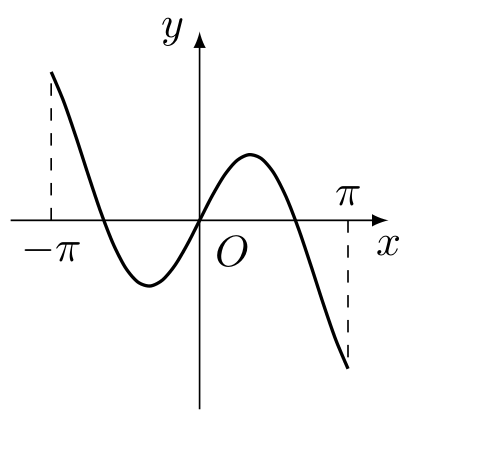
\includegraphics[width=0.15\paperwidth]{GaoKao/images/2020/zhejiang/q4_choice_a.png}\)  &  \(\text{B. }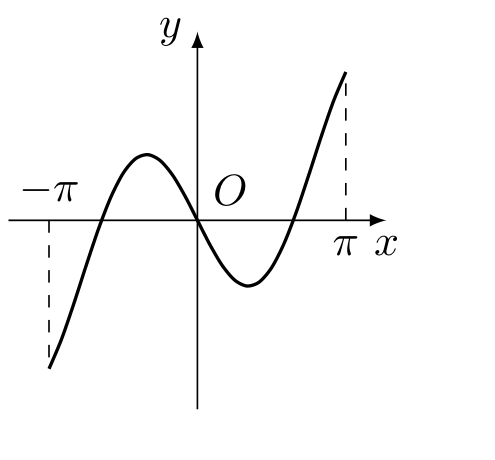
\includegraphics[width=0.15\paperwidth]{GaoKao/images/2020/zhejiang/q4_choice_b.png}\)  &  \(\text{C. }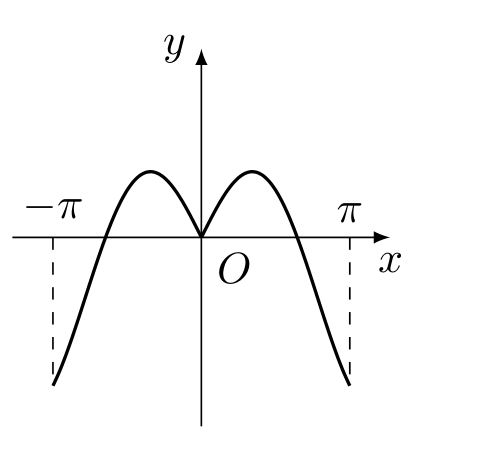
\includegraphics[width=0.15\paperwidth]{GaoKao/images/2020/zhejiang/q4_choice_c.png}\)  &  \(\text{D. }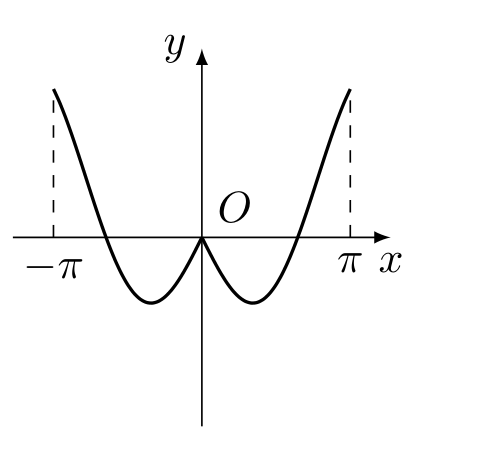
\includegraphics[width=0.15\paperwidth]{GaoKao/images/2020/zhejiang/q4_choice_d.png}\)
        \end{tabular*}\par}
        \item 某几何体的三视图（单位：cm）如图所示，则该几何体的体积（单位：$\text{cm}^{3}$）是（\quad）
        {\centering
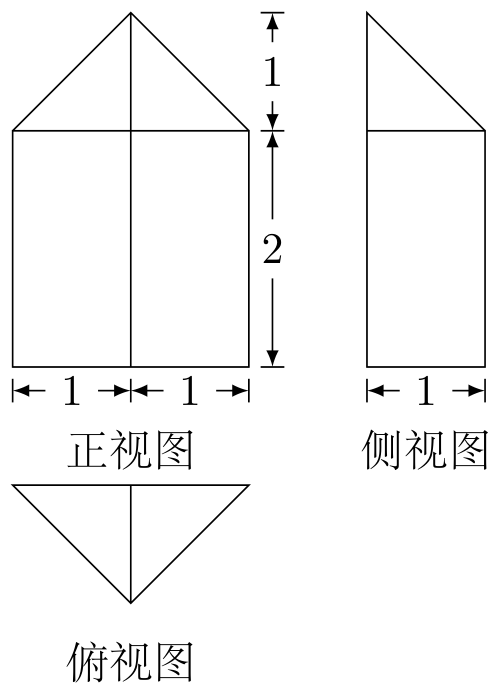
\includegraphics[width=4.9cm]{GaoKao/images/2020/zhejiang/q5_fig1.png}
\par}
        {\centering\begin{tabular*}{\linewidth}{@{}@{\extracolsep{\fill}}llll@{}}
            $\text{A. }\dfrac{7}{3}$  & $\text{B. }\dfrac{14}{3}$  & $\text{C. }3$  & $\text{D. }6$
        \end{tabular*}\par}        \item 已知空间中不过同一点的三条直线$m,n,l$，则``$m,n,l$在同一平面''是``$m,n,l$两两相交''的（\quad）
        {\centering\begin{tabular*}{\linewidth}{@{}@{\extracolsep{\fill}}llll@{}}
            $\text{A. }$充分不必要条件  & $\text{B. }$必要不充分条件  & $\text{C. }$充分必要条件  & $\text{D. }$既不充分也不必要条件
        \end{tabular*}\par}
        \item 已知等差数列$\{a_{n}\}$的前$n$项和$S_{n}$，公差$d\neq 0$，$\dfrac{a_{1}}{d}\leqslant 1$．记$b_{1}=S_{2}$，$b_{n+1}=S_{2n+2}-S_{2n}$，$n\in\mathbb{N}^{*}$，下列等式不可能成立的是（\quad）
        {\centering\begin{tabular*}{\linewidth}{@{}@{\extracolsep{\fill}}llll@{}}
            $\text{A. }2a_{4}=a_{2}+a_{6}$  & $\text{B. }2b_{4}=b_{2}+b_{6}$  & $\text{C. }a_{4}^{2}=a_{2}a_{8}$  & $\text{D. }b_{4}^{2}=b_{2}b_{8}$
        \end{tabular*}\par}
        \item 已知点$O(0,0)$，$A(-2,0)$，$B(2,0)$．设点$P$满足$|PA|-|PB|=2$，且$P$为函数$y=3\sqrt{4-x^{2}}$图象上的点，则$|OP|=$（\quad）
        {\centering\begin{tabular*}{\linewidth}{@{}@{\extracolsep{\fill}}llll@{}}
            $\text{A. }\dfrac{\sqrt{22}}{2}$  & $\text{B. }\dfrac{4\sqrt{10}}{5}$  & $\text{C. }\sqrt{7}$  & $\text{D. }\sqrt{10}$
        \end{tabular*}\par}
        \item 已知$a,b\in\mathbb{R}$且$ab\neq 0$，若$(x-a)(x-b)(x-2a-b)\geqslant 0$在$x\geqslant 0$上恒成立，则（\quad）
        {\centering\begin{tabular*}{\linewidth}{@{}@{\extracolsep{\fill}}llll@{}}
            $\text{A. }a<0$  & $\text{B. }a>0$  & $\text{C. }b<0$  & $\text{D. }b>0$
        \end{tabular*}\par}
        \item 设集合$S,T,S\subseteq\mathbb{N}^{*},T\subseteq\mathbb{N}^{*}$，$S,T$中至少有两个元素，且$S,T$满足：\\
        \ding{172}对于任意$x,y\in S$，若$x\neq y$，都有$xy\in T$；\\
        \ding{173}对于任意$x,y\in T$，若$x<y$，则$\dfrac{y}{x}\in S$．\\
        下列命题正确的是（\quad）
        {\centering\begin{tabular*}{\linewidth}{@{}@{\extracolsep{\fill}}llll@{}}
            $\text{A. }$若$S$有$4$个元素，则$S\cup T$有$7$个元素  & $\text{B. }$若$S$有$4$个元素，则$S\cup T$有$6$个元素  & $\text{C. }$若$S$有$3$个元素，则$S\cup T$有$4$个元素  & $\text{D. }$若$S$有$3$个元素，则$S\cup T$有$5$个元素
        \end{tabular*}\par}
    \end{enumerate}    \item[二、填空题]
    \begin{enumerate}[leftmargin=5pt]
      \addtocounter{enumi}{+10}
        \item 已知数列$\{a_{n}\}$满足$a_{n}=\dfrac{n(n+1)}{2}$，则$S_{3}=\rule[-0.3ex]{3em}{0.4pt}$．
        \item 设$(1+2x)^{5}=a_{1}+a_{2}x+a_{3}x^{2}+a_{4}x^{3}+a_{5}x^{4}+a_{6}x^{5}$，则$a_{5}=\rule[-0.3ex]{3em}{0.4pt}$；$a_{1}+a_{2}+a_{3}=\rule[-0.3ex]{3em}{0.4pt}$．
        \item 已知$\tan\theta=2$，则$\cos2\theta=\rule[-0.3ex]{3em}{0.4pt}$；$\tan\bigl(\theta-\frac{\pi}{4}\bigr)=\rule[-0.3ex]{3em}{0.4pt}$．
        \item 已知圆锥展开图的侧面积为$2\pi$，且为半圆，则底面半径为\rule[-0.3ex]{3em}{0.4pt}．
        \item 设直线$l:y=kx+b$（$k>0$），圆$C_{1}:x^{2}+y^{2}=1$，$C_{2}:(x-4)^{2}+y^{2}=1$，若直线$l$与$C_{1}$，$C_{2}$都相切，则$k=\rule[-0.3ex]{3em}{0.4pt}$；$b=\rule[-0.3ex]{3em}{0.4pt}$．
        \item 设$\bm{e}_{1},\bm{e}_{2}$为单位向量，满足$|2\bm{e}_{1}-\bm{e}_{2}|\leqslant\sqrt{2}$，$\bm{a}=\bm{e}_{1}+\bm{e}_{2}$，$\bm{b}=3\bm{e}_{1}+\bm{e}_{2}$，设$\bm{a},\bm{b}$的夹角为$\theta$，则$\cos^{2}\theta$的最小值为\rule[-0.3ex]{3em}{0.4pt}．
    \end{enumerate}
    \item[三、解答题]
    \begin{enumerate}[leftmargin=5pt]
      \addtocounter{enumi}{+17}
        \item 在锐角$\triangle ABC$中，角$A,B,C$的对边分别为$a,b,c$，且$2b\sin A=\sqrt{3}a$．
        \begin{enumerate}[label=(\arabic*)]
            \item 求角$B$；
            \item 求$\cos A+\cos B+\cos C$的取值范围．
        \end{enumerate}
        \item 如图，三棱台$DEF-ABC$中，面$ADFC\perp$面$ABC$，$\angle ACB=\angle ACD=45^{\circ}$，$DC=2BC$．
        \begin{enumerate}[label=(\arabic*)]
            \item 证明：$EF\perp DB$；
            \item 求$DF$与面$DBC$所成角的正弦值．
        \end{enumerate}        \item 已知数列$\{a_{n}\}$，$\{b_{n}\}$，$\{c_{n}\}$中，$a_{1}=b_{1}=c_{1}=1$，$c_{n}=a_{n+1}-a_{n}$，$c_{n+1}=\dfrac{b_{n}}{b_{n+2}}\cdot c_{n}$，$n\in\mathbb{N}^{*}$．
        \begin{enumerate}[label=(\arabic*)]
            \item 若数列$\{b_{n}\}$为等比数列，且公比$q>0$，且$b_{1}+b_{2}=6b_{3}$，求$q$与$a_{n}$通项公式；
            \item 若数列$\{b_{n}\}$为等差数列，且公差$d>0$，证明：$c_{1}+c_{2}+\cdots+c_{n}<1+\dfrac{1}{d}$，$n\in\mathbb{N}^{*}$．
        \end{enumerate}
        \item 如图，已知椭圆$C_{1}:\dfrac{x^{2}}{2}+y^{2}=1$，抛物线$C_{2}:y^{2}=2px$（$p>0$），点$A$是椭圆$C_{1}$与抛物线$C_{2}$的交点，过点$A$的直线$l$交椭圆$C_{1}$于点$B$，交抛物线$C_{2}$于$M$（$B,M$不同于$A$）．
        \begin{enumerate}[label=(\arabic*)]
            \item 若$p=\dfrac{1}{16}$，求抛物线$C_{2}$的焦点坐标；
            \item 若存在不过原点的直线$l$使$M$为线段$AB$的中点，求$p$的最大值．
        \end{enumerate}
        \item 已知$1<a\leqslant 2$，函数$f(x)=\mathrm{e}^{x}-x-a$，其中$\mathrm{e}=2.71828\cdots$为自然对数的底数．
        \begin{enumerate}[label=(\arabic*)]
            \item 证明：函数$y=f(x)$在$(0,+\infty)$上有唯一零点；
            \item 设$x_{0}$为函数$y=f(x)$在$(0,+\infty)$上的零点，证明：\\
            \ding{172}$\sqrt{a-1}\leqslant x_{0}\leqslant\sqrt{2(a-1)}$；\\
            \ding{173}$x_{0}f(\mathrm{e}^{x_{0}})\geqslant(\mathrm{e}-1)(a-1)a$．
        \end{enumerate}
    \end{enumerate}
\end{description}
\clearpage
